\documentclass[12pt]{report}

% import and apply GIRS "formatting.sty" file
\usepackage{import}
\usepackage{formatting}

% load hyperref last to minimize conflicts
\usepackage{xcolor}
\usepackage{tikz}
\usetikzlibrary{arrows.meta, positioning}
\usepackage[linktocpage=true]{hyperref}
\hypersetup{colorlinks=true, linkcolor=blue, citecolor=blue}

%-------------------------------------------------------
% Report helpers (CAP 5410 final report)
% \todo{...}  visible red marker for every part that is not finished / not run yet
% \nr         "not run" cell in a generated table
% \res{key}   a number from the CSV logs, defined in generated/numbers.tex
%             (written by make_figures.py). A missing key prints a red ??key.
\DeclareRobustCommand{\todo}[1]{{\color{red}\textbf{[TODO:} #1\textbf{]}}}
\DeclareRobustCommand{\nr}{\textcolor{red}{n/r}}
\newcommand{\res}[1]{\ifcsname res:#1\endcsname\csname res:#1\endcsname\else\textcolor{red}{\textbf{??\detokenize{#1}}}\fi}
% generated by report/make_figures.py - do not edit by hand
\expandafter\def\csname res:app-clip-hits\endcsname{7}
\expandafter\def\csname res:app-clip-hits-len\endcsname{7}
\expandafter\def\csname res:app-clip-ja-SV9-101-pred\endcsname{ja-SV9-101}
\expandafter\def\csname res:app-clip-ja-SV9-101-rank\endcsname{1}
\expandafter\def\csname res:app-clip-ja-SV9-106-pred\endcsname{ja-SV9-106}
\expandafter\def\csname res:app-clip-ja-SV9-106-rank\endcsname{1}
\expandafter\def\csname res:app-clip-me5-102-pred\endcsname{me5-102}
\expandafter\def\csname res:app-clip-me5-102-rank\endcsname{1}
\expandafter\def\csname res:app-clip-me5-115-pred\endcsname{me5-115}
\expandafter\def\csname res:app-clip-me5-115-rank\endcsname{1}
\expandafter\def\csname res:app-clip-me5-87-pred\endcsname{me5-87}
\expandafter\def\csname res:app-clip-me5-87-rank\endcsname{1}
\expandafter\def\csname res:app-clip-me5-92-pred\endcsname{me5-92}
\expandafter\def\csname res:app-clip-me5-92-rank\endcsname{1}
\expandafter\def\csname res:app-clip-me5-94-pred\endcsname{me5-94}
\expandafter\def\csname res:app-clip-me5-94-rank\endcsname{1}
\expandafter\def\csname res:app-clip-ms\endcsname{270}
\expandafter\def\csname res:app-cond-max\endcsname{320}
\expandafter\def\csname res:app-cond-min\endcsname{132}
\expandafter\def\csname res:app-hybrid_clip+rot_k20-hits\endcsname{7}
\expandafter\def\csname res:app-hybrid_clip+rot_k20-hits-len\endcsname{7}
\expandafter\def\csname res:app-hybrid_clip+rot_k20-ja-SV9-101-pred\endcsname{ja-SV9-101}
\expandafter\def\csname res:app-hybrid_clip+rot_k20-ja-SV9-101-rank\endcsname{1}
\expandafter\def\csname res:app-hybrid_clip+rot_k20-ja-SV9-106-pred\endcsname{ja-SV9-106}
\expandafter\def\csname res:app-hybrid_clip+rot_k20-ja-SV9-106-rank\endcsname{1}
\expandafter\def\csname res:app-hybrid_clip+rot_k20-me5-102-pred\endcsname{me5-102}
\expandafter\def\csname res:app-hybrid_clip+rot_k20-me5-102-rank\endcsname{1}
\expandafter\def\csname res:app-hybrid_clip+rot_k20-me5-115-pred\endcsname{me5-115}
\expandafter\def\csname res:app-hybrid_clip+rot_k20-me5-115-rank\endcsname{1}
\expandafter\def\csname res:app-hybrid_clip+rot_k20-me5-87-pred\endcsname{me5-87}
\expandafter\def\csname res:app-hybrid_clip+rot_k20-me5-87-rank\endcsname{1}
\expandafter\def\csname res:app-hybrid_clip+rot_k20-me5-92-pred\endcsname{me5-92}
\expandafter\def\csname res:app-hybrid_clip+rot_k20-me5-92-rank\endcsname{1}
\expandafter\def\csname res:app-hybrid_clip+rot_k20-me5-94-pred\endcsname{me5-94}
\expandafter\def\csname res:app-hybrid_clip+rot_k20-me5-94-rank\endcsname{1}
\expandafter\def\csname res:app-hybrid_clip+rot_k20-ms\endcsname{1,015}
\expandafter\def\csname res:app-hybrid_clip@art+rot_k20-hits\endcsname{5}
\expandafter\def\csname res:app-hybrid_clip@art+rot_k20-hits-len\endcsname{7}
\expandafter\def\csname res:app-hybrid_clip@art+rot_k20-ja-SV9-101-pred\endcsname{sv9-160}
\expandafter\def\csname res:app-hybrid_clip@art+rot_k20-ja-SV9-101-rank\endcsname{2}
\expandafter\def\csname res:app-hybrid_clip@art+rot_k20-ja-SV9-106-pred\endcsname{sv9-165}
\expandafter\def\csname res:app-hybrid_clip@art+rot_k20-ja-SV9-106-rank\endcsname{2}
\expandafter\def\csname res:app-hybrid_clip@art+rot_k20-me5-102-pred\endcsname{me5-102}
\expandafter\def\csname res:app-hybrid_clip@art+rot_k20-me5-102-rank\endcsname{1}
\expandafter\def\csname res:app-hybrid_clip@art+rot_k20-me5-115-pred\endcsname{me5-115}
\expandafter\def\csname res:app-hybrid_clip@art+rot_k20-me5-115-rank\endcsname{1}
\expandafter\def\csname res:app-hybrid_clip@art+rot_k20-me5-87-pred\endcsname{me5-87}
\expandafter\def\csname res:app-hybrid_clip@art+rot_k20-me5-87-rank\endcsname{1}
\expandafter\def\csname res:app-hybrid_clip@art+rot_k20-me5-92-pred\endcsname{me5-92}
\expandafter\def\csname res:app-hybrid_clip@art+rot_k20-me5-92-rank\endcsname{1}
\expandafter\def\csname res:app-hybrid_clip@art+rot_k20-me5-94-pred\endcsname{me5-94}
\expandafter\def\csname res:app-hybrid_clip@art+rot_k20-me5-94-rank\endcsname{1}
\expandafter\def\csname res:app-hybrid_clip@art+rot_k20-ms\endcsname{735}
\expandafter\def\csname res:app-ja-SV9-101-back-centering\endcsname{695}
\expandafter\def\csname res:app-ja-SV9-101-back-corners\endcsname{152}
\expandafter\def\csname res:app-ja-SV9-101-back-edges\endcsname{167}
\expandafter\def\csname res:app-ja-SV9-101-back-inliers\endcsname{0}
\expandafter\def\csname res:app-ja-SV9-101-back-ndefects\endcsname{0}
\expandafter\def\csname res:app-ja-SV9-101-back-overall\endcsname{302}
\expandafter\def\csname res:app-ja-SV9-101-cond\endcsname{261}
\expandafter\def\csname res:app-ja-SV9-101-found\endcsname{yes}
\expandafter\def\csname res:app-ja-SV9-101-front-centering\endcsname{779}
\expandafter\def\csname res:app-ja-SV9-101-front-corners\endcsname{214}
\expandafter\def\csname res:app-ja-SV9-101-front-edges\endcsname{0}
\expandafter\def\csname res:app-ja-SV9-101-front-inliers\endcsname{459}
\expandafter\def\csname res:app-ja-SV9-101-front-ndefects\endcsname{115}
\expandafter\def\csname res:app-ja-SV9-101-front-overall\endcsname{220}
\expandafter\def\csname res:app-ja-SV9-101-front-surface\endcsname{0}
\expandafter\def\csname res:app-ja-SV9-101-price\endcsname{1.33}
\expandafter\def\csname res:app-ja-SV9-101-score\endcsname{251}
\expandafter\def\csname res:app-ja-SV9-101-sift-second\endcsname{74}
\expandafter\def\csname res:app-ja-SV9-101-sift-top1\endcsname{251}
\expandafter\def\csname res:app-ja-SV9-106-back-centering\endcsname{253}
\expandafter\def\csname res:app-ja-SV9-106-back-corners\endcsname{53}
\expandafter\def\csname res:app-ja-SV9-106-back-edges\endcsname{276}
\expandafter\def\csname res:app-ja-SV9-106-back-inliers\endcsname{0}
\expandafter\def\csname res:app-ja-SV9-106-back-ndefects\endcsname{0}
\expandafter\def\csname res:app-ja-SV9-106-back-overall\endcsname{181}
\expandafter\def\csname res:app-ja-SV9-106-cond\endcsname{189}
\expandafter\def\csname res:app-ja-SV9-106-found\endcsname{yes}
\expandafter\def\csname res:app-ja-SV9-106-front-centering\endcsname{658}
\expandafter\def\csname res:app-ja-SV9-106-front-corners\endcsname{0}
\expandafter\def\csname res:app-ja-SV9-106-front-edges\endcsname{64}
\expandafter\def\csname res:app-ja-SV9-106-front-inliers\endcsname{582}
\expandafter\def\csname res:app-ja-SV9-106-front-ndefects\endcsname{0}
\expandafter\def\csname res:app-ja-SV9-106-front-overall\endcsname{197}
\expandafter\def\csname res:app-ja-SV9-106-price\endcsname{1.60}
\expandafter\def\csname res:app-ja-SV9-106-score\endcsname{290}
\expandafter\def\csname res:app-ja-SV9-106-sift-second\endcsname{87}
\expandafter\def\csname res:app-ja-SV9-106-sift-top1\endcsname{290}
\expandafter\def\csname res:app-me5-102-back-centering\endcsname{923}
\expandafter\def\csname res:app-me5-102-back-corners\endcsname{0}
\expandafter\def\csname res:app-me5-102-back-edges\endcsname{0}
\expandafter\def\csname res:app-me5-102-back-inliers\endcsname{0}
\expandafter\def\csname res:app-me5-102-back-ndefects\endcsname{0}
\expandafter\def\csname res:app-me5-102-back-overall\endcsname{246}
\expandafter\def\csname res:app-me5-102-cond\endcsname{258}
\expandafter\def\csname res:app-me5-102-found\endcsname{yes}
\expandafter\def\csname res:app-me5-102-front-centering\endcsname{483}
\expandafter\def\csname res:app-me5-102-front-corners\endcsname{198}
\expandafter\def\csname res:app-me5-102-front-edges\endcsname{182}
\expandafter\def\csname res:app-me5-102-front-inliers\endcsname{462}
\expandafter\def\csname res:app-me5-102-front-ndefects\endcsname{0}
\expandafter\def\csname res:app-me5-102-front-overall\endcsname{269}
\expandafter\def\csname res:app-me5-102-price\endcsname{3.52}
\expandafter\def\csname res:app-me5-102-score\endcsname{285}
\expandafter\def\csname res:app-me5-102-sift-second\endcsname{136}
\expandafter\def\csname res:app-me5-102-sift-top1\endcsname{285}
\expandafter\def\csname res:app-me5-115-back-centering\endcsname{847}
\expandafter\def\csname res:app-me5-115-back-corners\endcsname{410}
\expandafter\def\csname res:app-me5-115-back-edges\endcsname{250}
\expandafter\def\csname res:app-me5-115-back-inliers\endcsname{0}
\expandafter\def\csname res:app-me5-115-back-ndefects\endcsname{0}
\expandafter\def\csname res:app-me5-115-back-overall\endcsname{473}
\expandafter\def\csname res:app-me5-115-cond\endcsname{320}
\expandafter\def\csname res:app-me5-115-found\endcsname{yes}
\expandafter\def\csname res:app-me5-115-front-centering\endcsname{836}
\expandafter\def\csname res:app-me5-115-front-corners\endcsname{0}
\expandafter\def\csname res:app-me5-115-front-edges\endcsname{0}
\expandafter\def\csname res:app-me5-115-front-inliers\endcsname{71}
\expandafter\def\csname res:app-me5-115-front-ndefects\endcsname{113}
\expandafter\def\csname res:app-me5-115-front-overall\endcsname{167}
\expandafter\def\csname res:app-me5-115-front-surface\endcsname{0}
\expandafter\def\csname res:app-me5-115-price\endcsname{32.39}
\expandafter\def\csname res:app-me5-115-score\endcsname{59}
\expandafter\def\csname res:app-me5-115-sift-second\endcsname{32}
\expandafter\def\csname res:app-me5-115-sift-top1\endcsname{59}
\expandafter\def\csname res:app-me5-87-back-centering\endcsname{166}
\expandafter\def\csname res:app-me5-87-back-corners\endcsname{0}
\expandafter\def\csname res:app-me5-87-back-edges\endcsname{177}
\expandafter\def\csname res:app-me5-87-back-inliers\endcsname{0}
\expandafter\def\csname res:app-me5-87-back-ndefects\endcsname{0}
\expandafter\def\csname res:app-me5-87-back-overall\endcsname{103}
\expandafter\def\csname res:app-me5-87-cond\endcsname{150}
\expandafter\def\csname res:app-me5-87-found\endcsname{yes}
\expandafter\def\csname res:app-me5-87-front-centering\endcsname{936}
\expandafter\def\csname res:app-me5-87-front-corners\endcsname{36}
\expandafter\def\csname res:app-me5-87-front-edges\endcsname{0}
\expandafter\def\csname res:app-me5-87-front-inliers\endcsname{295}
\expandafter\def\csname res:app-me5-87-front-ndefects\endcsname{33}
\expandafter\def\csname res:app-me5-87-front-overall\endcsname{198}
\expandafter\def\csname res:app-me5-87-front-surface\endcsname{0}
\expandafter\def\csname res:app-me5-87-price\endcsname{3.51}
\expandafter\def\csname res:app-me5-87-score\endcsname{202}
\expandafter\def\csname res:app-me5-87-sift-second\endcsname{65}
\expandafter\def\csname res:app-me5-87-sift-top1\endcsname{202}
\expandafter\def\csname res:app-me5-92-back-centering\endcsname{166}
\expandafter\def\csname res:app-me5-92-back-corners\endcsname{0}
\expandafter\def\csname res:app-me5-92-back-edges\endcsname{177}
\expandafter\def\csname res:app-me5-92-back-inliers\endcsname{0}
\expandafter\def\csname res:app-me5-92-back-ndefects\endcsname{0}
\expandafter\def\csname res:app-me5-92-back-overall\endcsname{103}
\expandafter\def\csname res:app-me5-92-cond\endcsname{136}
\expandafter\def\csname res:app-me5-92-found\endcsname{yes}
\expandafter\def\csname res:app-me5-92-front-centering\endcsname{661}
\expandafter\def\csname res:app-me5-92-front-corners\endcsname{126}
\expandafter\def\csname res:app-me5-92-front-edges\endcsname{0}
\expandafter\def\csname res:app-me5-92-front-inliers\endcsname{417}
\expandafter\def\csname res:app-me5-92-front-ndefects\endcsname{91}
\expandafter\def\csname res:app-me5-92-front-overall\endcsname{170}
\expandafter\def\csname res:app-me5-92-front-surface\endcsname{0}
\expandafter\def\csname res:app-me5-92-price\endcsname{1.31}
\expandafter\def\csname res:app-me5-92-score\endcsname{76.9}
\expandafter\def\csname res:app-me5-92-sift-second\endcsname{33}
\expandafter\def\csname res:app-me5-92-sift-top1\endcsname{251}
\expandafter\def\csname res:app-me5-94-back-centering\endcsname{166}
\expandafter\def\csname res:app-me5-94-back-corners\endcsname{0}
\expandafter\def\csname res:app-me5-94-back-edges\endcsname{177}
\expandafter\def\csname res:app-me5-94-back-inliers\endcsname{0}
\expandafter\def\csname res:app-me5-94-back-ndefects\endcsname{0}
\expandafter\def\csname res:app-me5-94-back-overall\endcsname{103}
\expandafter\def\csname res:app-me5-94-cond\endcsname{132}
\expandafter\def\csname res:app-me5-94-found\endcsname{yes}
\expandafter\def\csname res:app-me5-94-front-centering\endcsname{150}
\expandafter\def\csname res:app-me5-94-front-corners\endcsname{138}
\expandafter\def\csname res:app-me5-94-front-edges\endcsname{199}
\expandafter\def\csname res:app-me5-94-front-inliers\endcsname{469}
\expandafter\def\csname res:app-me5-94-front-ndefects\endcsname{0}
\expandafter\def\csname res:app-me5-94-front-overall\endcsname{162}
\expandafter\def\csname res:app-me5-94-price\endcsname{1.55}
\expandafter\def\csname res:app-me5-94-score\endcsname{82.9}
\expandafter\def\csname res:app-me5-94-sift-second\endcsname{125}
\expandafter\def\csname res:app-me5-94-sift-top1\endcsname{292}
\expandafter\def\csname res:app-n-cond\endcsname{7}
\expandafter\def\csname res:app-n-copies\endcsname{7}
\expandafter\def\csname res:app-n-en\endcsname{5}
\expandafter\def\csname res:app-n-items\endcsname{7}
\expandafter\def\csname res:app-n-ja\endcsname{2}
\expandafter\def\csname res:app-n-ref\endcsname{917}
\expandafter\def\csname res:app-orb-hits\endcsname{7}
\expandafter\def\csname res:app-orb-hits-len\endcsname{7}
\expandafter\def\csname res:app-orb-ja-SV9-101-pred\endcsname{ja-SV9-101}
\expandafter\def\csname res:app-orb-ja-SV9-101-rank\endcsname{1}
\expandafter\def\csname res:app-orb-ja-SV9-106-pred\endcsname{ja-SV9-106}
\expandafter\def\csname res:app-orb-ja-SV9-106-rank\endcsname{1}
\expandafter\def\csname res:app-orb-me5-102-pred\endcsname{me5-102}
\expandafter\def\csname res:app-orb-me5-102-rank\endcsname{1}
\expandafter\def\csname res:app-orb-me5-115-pred\endcsname{me5-115}
\expandafter\def\csname res:app-orb-me5-115-rank\endcsname{1}
\expandafter\def\csname res:app-orb-me5-87-pred\endcsname{me5-87}
\expandafter\def\csname res:app-orb-me5-87-rank\endcsname{1}
\expandafter\def\csname res:app-orb-me5-92-pred\endcsname{me5-92}
\expandafter\def\csname res:app-orb-me5-92-rank\endcsname{1}
\expandafter\def\csname res:app-orb-me5-94-pred\endcsname{me5-94}
\expandafter\def\csname res:app-orb-me5-94-rank\endcsname{1}
\expandafter\def\csname res:app-orb-ms\endcsname{7,064}
\expandafter\def\csname res:app-pixel-hits\endcsname{3}
\expandafter\def\csname res:app-pixel-hits-len\endcsname{3}
\expandafter\def\csname res:app-pixel-ja-SV9-101-pred\endcsname{me2pt5-239}
\expandafter\def\csname res:app-pixel-ja-SV9-101-rank\endcsname{32}
\expandafter\def\csname res:app-pixel-ja-SV9-106-pred\endcsname{me2pt5-239}
\expandafter\def\csname res:app-pixel-ja-SV9-106-rank\endcsname{7}
\expandafter\def\csname res:app-pixel-me5-102-pred\endcsname{me5-102}
\expandafter\def\csname res:app-pixel-me5-102-rank\endcsname{1}
\expandafter\def\csname res:app-pixel-me5-115-pred\endcsname{me5-115}
\expandafter\def\csname res:app-pixel-me5-115-rank\endcsname{1}
\expandafter\def\csname res:app-pixel-me5-87-pred\endcsname{sv9-170}
\expandafter\def\csname res:app-pixel-me5-87-rank\endcsname{2}
\expandafter\def\csname res:app-pixel-me5-92-pred\endcsname{me5-52}
\expandafter\def\csname res:app-pixel-me5-92-rank\endcsname{22}
\expandafter\def\csname res:app-pixel-me5-94-pred\endcsname{me5-94}
\expandafter\def\csname res:app-pixel-me5-94-rank\endcsname{1}
\expandafter\def\csname res:app-pixel-ms\endcsname{142}
\expandafter\def\csname res:app-reid-n\endcsname{7}
\expandafter\def\csname res:app-resnet-hits\endcsname{5}
\expandafter\def\csname res:app-resnet-hits-len\endcsname{6}
\expandafter\def\csname res:app-resnet-ja-SV9-101-pred\endcsname{sv9-160}
\expandafter\def\csname res:app-resnet-ja-SV9-101-rank\endcsname{2}
\expandafter\def\csname res:app-resnet-ja-SV9-106-pred\endcsname{ja-SV9-106}
\expandafter\def\csname res:app-resnet-ja-SV9-106-rank\endcsname{1}
\expandafter\def\csname res:app-resnet-me5-102-pred\endcsname{me2pt5-282}
\expandafter\def\csname res:app-resnet-me5-102-rank\endcsname{191}
\expandafter\def\csname res:app-resnet-me5-115-pred\endcsname{me5-115}
\expandafter\def\csname res:app-resnet-me5-115-rank\endcsname{1}
\expandafter\def\csname res:app-resnet-me5-87-pred\endcsname{me5-87}
\expandafter\def\csname res:app-resnet-me5-87-rank\endcsname{1}
\expandafter\def\csname res:app-resnet-me5-92-pred\endcsname{me5-92}
\expandafter\def\csname res:app-resnet-me5-92-rank\endcsname{1}
\expandafter\def\csname res:app-resnet-me5-94-pred\endcsname{me5-94}
\expandafter\def\csname res:app-resnet-me5-94-rank\endcsname{1}
\expandafter\def\csname res:app-resnet-ms\endcsname{275}
\expandafter\def\csname res:app-sift-hits\endcsname{7}
\expandafter\def\csname res:app-sift-hits-len\endcsname{7}
\expandafter\def\csname res:app-sift-ja-SV9-101-pred\endcsname{ja-SV9-101}
\expandafter\def\csname res:app-sift-ja-SV9-101-rank\endcsname{1}
\expandafter\def\csname res:app-sift-ja-SV9-106-pred\endcsname{ja-SV9-106}
\expandafter\def\csname res:app-sift-ja-SV9-106-rank\endcsname{1}
\expandafter\def\csname res:app-sift-me5-102-pred\endcsname{me5-102}
\expandafter\def\csname res:app-sift-me5-102-rank\endcsname{1}
\expandafter\def\csname res:app-sift-me5-115-pred\endcsname{me5-115}
\expandafter\def\csname res:app-sift-me5-115-rank\endcsname{1}
\expandafter\def\csname res:app-sift-me5-87-pred\endcsname{me5-87}
\expandafter\def\csname res:app-sift-me5-87-rank\endcsname{1}
\expandafter\def\csname res:app-sift-me5-92-pred\endcsname{me5-92}
\expandafter\def\csname res:app-sift-me5-92-rank\endcsname{1}
\expandafter\def\csname res:app-sift-me5-94-pred\endcsname{me5-94}
\expandafter\def\csname res:app-sift-me5-94-rank\endcsname{1}
\expandafter\def\csname res:app-sift-ms\endcsname{22,329}
\expandafter\def\csname res:app-snapshot-date\endcsname{2026-11-08}
\expandafter\def\csname res:app-total-eur\endcsname{2.93}
\expandafter\def\csname res:app-total-usd\endcsname{42.28}
\expandafter\def\csname res:clip+rot-s1-mAP\endcsname{0.985}
\expandafter\def\csname res:clip+rot-s1-ms\endcsname{135}
\expandafter\def\csname res:clip+rot-s1-msrect\endcsname{91}
\expandafter\def\csname res:clip+rot-s1-n\endcsname{200}
\expandafter\def\csname res:clip+rot-s1-nbadrect\endcsname{3}
\expandafter\def\csname res:clip+rot-s1-nfailed\endcsname{6}
\expandafter\def\csname res:clip+rot-s1-rect_ok\endcsname{0.985}
\expandafter\def\csname res:clip+rot-s1-rectify_found\endcsname{1.000}
\expandafter\def\csname res:clip+rot-s1-top1\endcsname{0.970}
\expandafter\def\csname res:clip+rot-s1-top1_given_bad_rect\endcsname{1.000}
\expandafter\def\csname res:clip+rot-s1-top1_given_rect\endcsname{0.970}
\expandafter\def\csname res:clip+rot-s1-top1_hi\endcsname{0.990}
\expandafter\def\csname res:clip+rot-s1-top1_len\endcsname{1.000}
\expandafter\def\csname res:clip+rot-s1-top1_lo\endcsname{0.945}
\expandafter\def\csname res:clip+rot-s1-top5\endcsname{1.000}
\expandafter\def\csname res:clip+rot-s2-mAP\endcsname{0.972}
\expandafter\def\csname res:clip+rot-s2-ms\endcsname{156}
\expandafter\def\csname res:clip+rot-s2-msrect\endcsname{95}
\expandafter\def\csname res:clip+rot-s2-n\endcsname{200}
\expandafter\def\csname res:clip+rot-s2-nbadrect\endcsname{2}
\expandafter\def\csname res:clip+rot-s2-nfailed\endcsname{10}
\expandafter\def\csname res:clip+rot-s2-rect_ok\endcsname{0.990}
\expandafter\def\csname res:clip+rot-s2-rectify_found\endcsname{1.000}
\expandafter\def\csname res:clip+rot-s2-top1\endcsname{0.950}
\expandafter\def\csname res:clip+rot-s2-top1_given_bad_rect\endcsname{0.500}
\expandafter\def\csname res:clip+rot-s2-top1_given_rect\endcsname{0.955}
\expandafter\def\csname res:clip+rot-s2-top1_hi\endcsname{0.975}
\expandafter\def\csname res:clip+rot-s2-top1_len\endcsname{0.990}
\expandafter\def\csname res:clip+rot-s2-top1_lo\endcsname{0.920}
\expandafter\def\csname res:clip+rot-s2-top5\endcsname{0.995}
\expandafter\def\csname res:clip+rot-s3-mAP\endcsname{0.862}
\expandafter\def\csname res:clip+rot-s3-ms\endcsname{138}
\expandafter\def\csname res:clip+rot-s3-msrect\endcsname{86}
\expandafter\def\csname res:clip+rot-s3-n\endcsname{200}
\expandafter\def\csname res:clip+rot-s3-nbadrect\endcsname{4}
\expandafter\def\csname res:clip+rot-s3-nfailed\endcsname{38}
\expandafter\def\csname res:clip+rot-s3-rect_ok\endcsname{0.980}
\expandafter\def\csname res:clip+rot-s3-rectify_found\endcsname{1.000}
\expandafter\def\csname res:clip+rot-s3-top1\endcsname{0.810}
\expandafter\def\csname res:clip+rot-s3-top1_given_bad_rect\endcsname{0.250}
\expandafter\def\csname res:clip+rot-s3-top1_given_rect\endcsname{0.821}
\expandafter\def\csname res:clip+rot-s3-top1_hi\endcsname{0.865}
\expandafter\def\csname res:clip+rot-s3-top1_len\endcsname{0.840}
\expandafter\def\csname res:clip+rot-s3-top1_lo\endcsname{0.760}
\expandafter\def\csname res:clip+rot-s3-top5\endcsname{0.920}
\expandafter\def\csname res:clip+rot-s4-mAP\endcsname{0.369}
\expandafter\def\csname res:clip+rot-s4-ms\endcsname{180}
\expandafter\def\csname res:clip+rot-s4-msrect\endcsname{98}
\expandafter\def\csname res:clip+rot-s4-n\endcsname{200}
\expandafter\def\csname res:clip+rot-s4-nbadrect\endcsname{22}
\expandafter\def\csname res:clip+rot-s4-nfailed\endcsname{145}
\expandafter\def\csname res:clip+rot-s4-rect_ok\endcsname{0.890}
\expandafter\def\csname res:clip+rot-s4-rectify_found\endcsname{0.910}
\expandafter\def\csname res:clip+rot-s4-top1\endcsname{0.275}
\expandafter\def\csname res:clip+rot-s4-top1_given_bad_rect\endcsname{0.045}
\expandafter\def\csname res:clip+rot-s4-top1_given_rect\endcsname{0.303}
\expandafter\def\csname res:clip+rot-s4-top1_hi\endcsname{0.335}
\expandafter\def\csname res:clip+rot-s4-top1_len\endcsname{0.280}
\expandafter\def\csname res:clip+rot-s4-top1_lo\endcsname{0.210}
\expandafter\def\csname res:clip+rot-s4-top5\endcsname{0.460}
\expandafter\def\csname res:clip+rot-s5-mAP\endcsname{0.036}
\expandafter\def\csname res:clip+rot-s5-ms\endcsname{201}
\expandafter\def\csname res:clip+rot-s5-msrect\endcsname{112}
\expandafter\def\csname res:clip+rot-s5-n\endcsname{200}
\expandafter\def\csname res:clip+rot-s5-nbadrect\endcsname{146}
\expandafter\def\csname res:clip+rot-s5-nfailed\endcsname{196}
\expandafter\def\csname res:clip+rot-s5-rect_ok\endcsname{0.270}
\expandafter\def\csname res:clip+rot-s5-rectify_found\endcsname{0.360}
\expandafter\def\csname res:clip+rot-s5-top1\endcsname{0.020}
\expandafter\def\csname res:clip+rot-s5-top1_given_bad_rect\endcsname{0.007}
\expandafter\def\csname res:clip+rot-s5-top1_given_rect\endcsname{0.056}
\expandafter\def\csname res:clip+rot-s5-top1_hi\endcsname{0.040}
\expandafter\def\csname res:clip+rot-s5-top1_len\endcsname{0.020}
\expandafter\def\csname res:clip+rot-s5-top1_lo\endcsname{0.005}
\expandafter\def\csname res:clip+rot-s5-top5\endcsname{0.035}
\expandafter\def\csname res:clip-s1-mAP\endcsname{0.985}
\expandafter\def\csname res:clip-s1-ms\endcsname{140}
\expandafter\def\csname res:clip-s1-msrect\endcsname{98}
\expandafter\def\csname res:clip-s1-n\endcsname{200}
\expandafter\def\csname res:clip-s1-nbadrect\endcsname{3}
\expandafter\def\csname res:clip-s1-nfailed\endcsname{6}
\expandafter\def\csname res:clip-s1-rect_ok\endcsname{0.985}
\expandafter\def\csname res:clip-s1-rectify_found\endcsname{1.000}
\expandafter\def\csname res:clip-s1-top1\endcsname{0.970}
\expandafter\def\csname res:clip-s1-top1_given_bad_rect\endcsname{1.000}
\expandafter\def\csname res:clip-s1-top1_given_rect\endcsname{0.970}
\expandafter\def\csname res:clip-s1-top1_hi\endcsname{0.990}
\expandafter\def\csname res:clip-s1-top1_len\endcsname{1.000}
\expandafter\def\csname res:clip-s1-top1_lo\endcsname{0.945}
\expandafter\def\csname res:clip-s1-top5\endcsname{1.000}
\expandafter\def\csname res:clip-s2-mAP\endcsname{0.975}
\expandafter\def\csname res:clip-s2-ms\endcsname{141}
\expandafter\def\csname res:clip-s2-msrect\endcsname{102}
\expandafter\def\csname res:clip-s2-n\endcsname{200}
\expandafter\def\csname res:clip-s2-nbadrect\endcsname{2}
\expandafter\def\csname res:clip-s2-nfailed\endcsname{9}
\expandafter\def\csname res:clip-s2-rect_ok\endcsname{0.990}
\expandafter\def\csname res:clip-s2-rectify_found\endcsname{1.000}
\expandafter\def\csname res:clip-s2-top1\endcsname{0.955}
\expandafter\def\csname res:clip-s2-top1_given_bad_rect\endcsname{0.500}
\expandafter\def\csname res:clip-s2-top1_given_rect\endcsname{0.960}
\expandafter\def\csname res:clip-s2-top1_hi\endcsname{0.980}
\expandafter\def\csname res:clip-s2-top1_len\endcsname{0.995}
\expandafter\def\csname res:clip-s2-top1_lo\endcsname{0.925}
\expandafter\def\csname res:clip-s2-top5\endcsname{0.995}
\expandafter\def\csname res:clip-s3-mAP\endcsname{0.887}
\expandafter\def\csname res:clip-s3-ms\endcsname{165}
\expandafter\def\csname res:clip-s3-msrect\endcsname{113}
\expandafter\def\csname res:clip-s3-n\endcsname{200}
\expandafter\def\csname res:clip-s3-nbadrect\endcsname{4}
\expandafter\def\csname res:clip-s3-nfailed\endcsname{31}
\expandafter\def\csname res:clip-s3-rect_ok\endcsname{0.980}
\expandafter\def\csname res:clip-s3-rectify_found\endcsname{1.000}
\expandafter\def\csname res:clip-s3-top1\endcsname{0.845}
\expandafter\def\csname res:clip-s3-top1_given_bad_rect\endcsname{0.250}
\expandafter\def\csname res:clip-s3-top1_given_rect\endcsname{0.857}
\expandafter\def\csname res:clip-s3-top1_hi\endcsname{0.895}
\expandafter\def\csname res:clip-s3-top1_len\endcsname{0.875}
\expandafter\def\csname res:clip-s3-top1_lo\endcsname{0.790}
\expandafter\def\csname res:clip-s3-top5\endcsname{0.930}
\expandafter\def\csname res:clip-s4-mAP\endcsname{0.349}
\expandafter\def\csname res:clip-s4-ms\endcsname{154}
\expandafter\def\csname res:clip-s4-msrect\endcsname{111}
\expandafter\def\csname res:clip-s4-n\endcsname{200}
\expandafter\def\csname res:clip-s4-nbadrect\endcsname{22}
\expandafter\def\csname res:clip-s4-nfailed\endcsname{150}
\expandafter\def\csname res:clip-s4-rect_ok\endcsname{0.890}
\expandafter\def\csname res:clip-s4-rectify_found\endcsname{0.910}
\expandafter\def\csname res:clip-s4-top1\endcsname{0.250}
\expandafter\def\csname res:clip-s4-top1_given_bad_rect\endcsname{0.045}
\expandafter\def\csname res:clip-s4-top1_given_rect\endcsname{0.275}
\expandafter\def\csname res:clip-s4-top1_hi\endcsname{0.305}
\expandafter\def\csname res:clip-s4-top1_len\endcsname{0.255}
\expandafter\def\csname res:clip-s4-top1_lo\endcsname{0.185}
\expandafter\def\csname res:clip-s4-top5\endcsname{0.445}
\expandafter\def\csname res:clip-s5-mAP\endcsname{0.032}
\expandafter\def\csname res:clip-s5-ms\endcsname{171}
\expandafter\def\csname res:clip-s5-msrect\endcsname{127}
\expandafter\def\csname res:clip-s5-n\endcsname{200}
\expandafter\def\csname res:clip-s5-nbadrect\endcsname{146}
\expandafter\def\csname res:clip-s5-nfailed\endcsname{196}
\expandafter\def\csname res:clip-s5-rect_ok\endcsname{0.270}
\expandafter\def\csname res:clip-s5-rectify_found\endcsname{0.360}
\expandafter\def\csname res:clip-s5-top1\endcsname{0.020}
\expandafter\def\csname res:clip-s5-top1_given_bad_rect\endcsname{0.007}
\expandafter\def\csname res:clip-s5-top1_given_rect\endcsname{0.056}
\expandafter\def\csname res:clip-s5-top1_hi\endcsname{0.040}
\expandafter\def\csname res:clip-s5-top1_len\endcsname{0.020}
\expandafter\def\csname res:clip-s5-top1_lo\endcsname{0.005}
\expandafter\def\csname res:clip-s5-top5\endcsname{0.025}
\expandafter\def\csname res:cond-aligned\endcsname{76}
\expandafter\def\csname res:cond-centering-lr-med\endcsname{0.58}
\expandafter\def\csname res:cond-centering-lr-p90\endcsname{2.33}
\expandafter\def\csname res:cond-centering-tb-med\endcsname{0.70}
\expandafter\def\csname res:cond-centering-tb-p90\endcsname{2.33}
\expandafter\def\csname res:cond-dev-n\endcsname{40}
\expandafter\def\csname res:cond-dev-overlap\endcsname{2}
\expandafter\def\csname res:cond-n\endcsname{80}
\expandafter\def\csname res:cond-overall\endcsname{-0.46}
\expandafter\def\csname res:cond-part-centering\endcsname{-0.90}
\expandafter\def\csname res:cond-part-corners\endcsname{-0.53}
\expandafter\def\csname res:cond-part-edges\endcsname{-0.32}
\expandafter\def\csname res:cond-part-surface\endcsname{-0.86}
\expandafter\def\csname res:cond-rectified\endcsname{80}
\expandafter\def\csname res:cond-rho-corner-cut\endcsname{-0.74}
\expandafter\def\csname res:cond-rho-corner-white\endcsname{+0.62}
\expandafter\def\csname res:cond-rho-edge-fray\endcsname{+0.41}
\expandafter\def\csname res:cond-rho-edge-white\endcsname{+0.78}
\expandafter\def\csname res:cond-surf-found\endcsname{68}
\expandafter\def\csname res:cond-surf-nest\endcsname{105}
\expandafter\def\csname res:cond-surf-ntrue\endcsname{111}
\expandafter\def\csname res:cond-surf-precision\endcsname{0.69}
\expandafter\def\csname res:cond-surf-real\endcsname{72}
\expandafter\def\csname res:cond-surf-recall\endcsname{0.61}
\expandafter\def\csname res:cond-surf-typed\endcsname{59}
\expandafter\def\csname res:db-art-maxart\endcsname{6}
\expandafter\def\csname res:db-art-maxfull\endcsname{2}
\expandafter\def\csname res:db-art-pairs\endcsname{24}
\expandafter\def\csname res:db-art-pairs-sv8pt5-me2pt5\endcsname{9}
\expandafter\def\csname res:db-art-pairs-sv9-me2pt5\endcsname{15}
\expandafter\def\csname res:db-artgroups\endcsname{761}
\expandafter\def\csname res:db-cards\endcsname{785}
\expandafter\def\csname res:db-dup-name-cards\endcsname{391}
\expandafter\def\csname res:db-dup-names\endcsname{163}
\expandafter\def\csname res:db-energy\endcsname{6}
\expandafter\def\csname res:db-ja-cards\endcsname{132}
\expandafter\def\csname res:db-ja-linked\endcsname{128}
\expandafter\def\csname res:db-max-name\endcsname{Black Belt's Training}
\expandafter\def\csname res:db-max-name-n\endcsname{8}
\expandafter\def\csname res:db-pokemon\endcsname{629}
\expandafter\def\csname res:db-sets\endcsname{4}
\expandafter\def\csname res:db-shared-groups\endcsname{24}
\expandafter\def\csname res:db-trainer\endcsname{150}
\expandafter\def\csname res:fail-clip+rot-heavydistortion\endcsname{171}
\expandafter\def\csname res:fail-clip+rot-heavydistortion-s4\endcsname{120}
\expandafter\def\csname res:fail-clip+rot-heavydistortion-s5\endcsname{51}
\expandafter\def\csname res:fail-clip+rot-localization\endcsname{163}
\expandafter\def\csname res:fail-clip+rot-localization-s2\endcsname{1}
\expandafter\def\csname res:fail-clip+rot-localization-s3\endcsname{2}
\expandafter\def\csname res:fail-clip+rot-localization-s4\endcsname{21}
\expandafter\def\csname res:fail-clip+rot-localization-s5\endcsname{139}
\expandafter\def\csname res:fail-clip+rot-lookalike\endcsname{5}
\expandafter\def\csname res:fail-clip+rot-lookalike-s3\endcsname{2}
\expandafter\def\csname res:fail-clip+rot-lookalike-s4\endcsname{3}
\expandafter\def\csname res:fail-clip+rot-other\endcsname{28}
\expandafter\def\csname res:fail-clip+rot-other-s2\endcsname{1}
\expandafter\def\csname res:fail-clip+rot-other-s3\endcsname{27}
\expandafter\def\csname res:fail-clip+rot-rectification\endcsname{7}
\expandafter\def\csname res:fail-clip+rot-rectification-s3\endcsname{1}
\expandafter\def\csname res:fail-clip+rot-rectification-s5\endcsname{6}
\expandafter\def\csname res:fail-clip+rot-s1\endcsname{6}
\expandafter\def\csname res:fail-clip+rot-s2\endcsname{10}
\expandafter\def\csname res:fail-clip+rot-s3\endcsname{38}
\expandafter\def\csname res:fail-clip+rot-s4\endcsname{145}
\expandafter\def\csname res:fail-clip+rot-s5\endcsname{196}
\expandafter\def\csname res:fail-clip+rot-sameartwork\endcsname{21}
\expandafter\def\csname res:fail-clip+rot-sameartwork-s1\endcsname{6}
\expandafter\def\csname res:fail-clip+rot-sameartwork-s2\endcsname{8}
\expandafter\def\csname res:fail-clip+rot-sameartwork-s3\endcsname{6}
\expandafter\def\csname res:fail-clip+rot-sameartwork-s4\endcsname{1}
\expandafter\def\csname res:fail-clip+rot-total\endcsname{395}
\expandafter\def\csname res:fail-clip+rot-upsidedown\endcsname{0}
\expandafter\def\csname res:fail-clip-heavydistortion\endcsname{136}
\expandafter\def\csname res:fail-clip-heavydistortion-s4\endcsname{109}
\expandafter\def\csname res:fail-clip-heavydistortion-s5\endcsname{27}
\expandafter\def\csname res:fail-clip-localization\endcsname{163}
\expandafter\def\csname res:fail-clip-localization-s2\endcsname{1}
\expandafter\def\csname res:fail-clip-localization-s3\endcsname{2}
\expandafter\def\csname res:fail-clip-localization-s4\endcsname{21}
\expandafter\def\csname res:fail-clip-localization-s5\endcsname{139}
\expandafter\def\csname res:fail-clip-lookalike\endcsname{7}
\expandafter\def\csname res:fail-clip-lookalike-s3\endcsname{4}
\expandafter\def\csname res:fail-clip-lookalike-s4\endcsname{3}
\expandafter\def\csname res:fail-clip-other\endcsname{18}
\expandafter\def\csname res:fail-clip-other-s3\endcsname{18}
\expandafter\def\csname res:fail-clip-rectification\endcsname{7}
\expandafter\def\csname res:fail-clip-rectification-s3\endcsname{1}
\expandafter\def\csname res:fail-clip-rectification-s5\endcsname{6}
\expandafter\def\csname res:fail-clip-s1\endcsname{6}
\expandafter\def\csname res:fail-clip-s2\endcsname{9}
\expandafter\def\csname res:fail-clip-s3\endcsname{31}
\expandafter\def\csname res:fail-clip-s4\endcsname{150}
\expandafter\def\csname res:fail-clip-s5\endcsname{196}
\expandafter\def\csname res:fail-clip-sameartwork\endcsname{21}
\expandafter\def\csname res:fail-clip-sameartwork-s1\endcsname{6}
\expandafter\def\csname res:fail-clip-sameartwork-s2\endcsname{8}
\expandafter\def\csname res:fail-clip-sameartwork-s3\endcsname{6}
\expandafter\def\csname res:fail-clip-sameartwork-s4\endcsname{1}
\expandafter\def\csname res:fail-clip-total\endcsname{392}
\expandafter\def\csname res:fail-clip-upsidedown\endcsname{40}
\expandafter\def\csname res:fail-clip-upsidedown-s4\endcsname{16}
\expandafter\def\csname res:fail-clip-upsidedown-s5\endcsname{24}
\expandafter\def\csname res:fail-hybrid_clip+rot_k20-heavydistortion\endcsname{111}
\expandafter\def\csname res:fail-hybrid_clip+rot_k20-heavydistortion-s4\endcsname{65}
\expandafter\def\csname res:fail-hybrid_clip+rot_k20-heavydistortion-s5\endcsname{46}
\expandafter\def\csname res:fail-hybrid_clip+rot_k20-localization\endcsname{163}
\expandafter\def\csname res:fail-hybrid_clip+rot_k20-localization-s2\endcsname{1}
\expandafter\def\csname res:fail-hybrid_clip+rot_k20-localization-s3\endcsname{2}
\expandafter\def\csname res:fail-hybrid_clip+rot_k20-localization-s4\endcsname{20}
\expandafter\def\csname res:fail-hybrid_clip+rot_k20-localization-s5\endcsname{140}
\expandafter\def\csname res:fail-hybrid_clip+rot_k20-lookalike\endcsname{1}
\expandafter\def\csname res:fail-hybrid_clip+rot_k20-lookalike-s4\endcsname{1}
\expandafter\def\csname res:fail-hybrid_clip+rot_k20-other\endcsname{9}
\expandafter\def\csname res:fail-hybrid_clip+rot_k20-other-s3\endcsname{9}
\expandafter\def\csname res:fail-hybrid_clip+rot_k20-rectification\endcsname{6}
\expandafter\def\csname res:fail-hybrid_clip+rot_k20-rectification-s5\endcsname{6}
\expandafter\def\csname res:fail-hybrid_clip+rot_k20-s1\endcsname{1}
\expandafter\def\csname res:fail-hybrid_clip+rot_k20-s2\endcsname{7}
\expandafter\def\csname res:fail-hybrid_clip+rot_k20-s3\endcsname{15}
\expandafter\def\csname res:fail-hybrid_clip+rot_k20-s4\endcsname{87}
\expandafter\def\csname res:fail-hybrid_clip+rot_k20-s5\endcsname{192}
\expandafter\def\csname res:fail-hybrid_clip+rot_k20-sameartwork\endcsname{12}
\expandafter\def\csname res:fail-hybrid_clip+rot_k20-sameartwork-s1\endcsname{1}
\expandafter\def\csname res:fail-hybrid_clip+rot_k20-sameartwork-s2\endcsname{6}
\expandafter\def\csname res:fail-hybrid_clip+rot_k20-sameartwork-s3\endcsname{4}
\expandafter\def\csname res:fail-hybrid_clip+rot_k20-sameartwork-s4\endcsname{1}
\expandafter\def\csname res:fail-hybrid_clip+rot_k20-total\endcsname{302}
\expandafter\def\csname res:fail-hybrid_clip+rot_k20-upsidedown\endcsname{0}
\expandafter\def\csname res:fail-hybrid_clip_k20-heavydistortion\endcsname{84}
\expandafter\def\csname res:fail-hybrid_clip_k20-heavydistortion-s4\endcsname{58}
\expandafter\def\csname res:fail-hybrid_clip_k20-heavydistortion-s5\endcsname{26}
\expandafter\def\csname res:fail-hybrid_clip_k20-localization\endcsname{163}
\expandafter\def\csname res:fail-hybrid_clip_k20-localization-s2\endcsname{1}
\expandafter\def\csname res:fail-hybrid_clip_k20-localization-s3\endcsname{2}
\expandafter\def\csname res:fail-hybrid_clip_k20-localization-s4\endcsname{20}
\expandafter\def\csname res:fail-hybrid_clip_k20-localization-s5\endcsname{140}
\expandafter\def\csname res:fail-hybrid_clip_k20-lookalike\endcsname{1}
\expandafter\def\csname res:fail-hybrid_clip_k20-lookalike-s4\endcsname{1}
\expandafter\def\csname res:fail-hybrid_clip_k20-other\endcsname{7}
\expandafter\def\csname res:fail-hybrid_clip_k20-other-s3\endcsname{7}
\expandafter\def\csname res:fail-hybrid_clip_k20-rectification\endcsname{6}
\expandafter\def\csname res:fail-hybrid_clip_k20-rectification-s5\endcsname{6}
\expandafter\def\csname res:fail-hybrid_clip_k20-s1\endcsname{1}
\expandafter\def\csname res:fail-hybrid_clip_k20-s2\endcsname{7}
\expandafter\def\csname res:fail-hybrid_clip_k20-s3\endcsname{13}
\expandafter\def\csname res:fail-hybrid_clip_k20-s4\endcsname{94}
\expandafter\def\csname res:fail-hybrid_clip_k20-s5\endcsname{196}
\expandafter\def\csname res:fail-hybrid_clip_k20-sameartwork\endcsname{12}
\expandafter\def\csname res:fail-hybrid_clip_k20-sameartwork-s1\endcsname{1}
\expandafter\def\csname res:fail-hybrid_clip_k20-sameartwork-s2\endcsname{6}
\expandafter\def\csname res:fail-hybrid_clip_k20-sameartwork-s3\endcsname{4}
\expandafter\def\csname res:fail-hybrid_clip_k20-sameartwork-s4\endcsname{1}
\expandafter\def\csname res:fail-hybrid_clip_k20-total\endcsname{311}
\expandafter\def\csname res:fail-hybrid_clip_k20-upsidedown\endcsname{38}
\expandafter\def\csname res:fail-hybrid_clip_k20-upsidedown-s4\endcsname{14}
\expandafter\def\csname res:fail-hybrid_clip_k20-upsidedown-s5\endcsname{24}
\expandafter\def\csname res:fail-hybrid_resnet+rot_k20-heavydistortion\endcsname{148}
\expandafter\def\csname res:fail-hybrid_resnet+rot_k20-heavydistortion-s4\endcsname{104}
\expandafter\def\csname res:fail-hybrid_resnet+rot_k20-heavydistortion-s5\endcsname{44}
\expandafter\def\csname res:fail-hybrid_resnet+rot_k20-localization\endcsname{161}
\expandafter\def\csname res:fail-hybrid_resnet+rot_k20-localization-s2\endcsname{1}
\expandafter\def\csname res:fail-hybrid_resnet+rot_k20-localization-s3\endcsname{1}
\expandafter\def\csname res:fail-hybrid_resnet+rot_k20-localization-s4\endcsname{21}
\expandafter\def\csname res:fail-hybrid_resnet+rot_k20-localization-s5\endcsname{138}
\expandafter\def\csname res:fail-hybrid_resnet+rot_k20-lookalike\endcsname{3}
\expandafter\def\csname res:fail-hybrid_resnet+rot_k20-lookalike-s2\endcsname{1}
\expandafter\def\csname res:fail-hybrid_resnet+rot_k20-lookalike-s3\endcsname{1}
\expandafter\def\csname res:fail-hybrid_resnet+rot_k20-lookalike-s5\endcsname{1}
\expandafter\def\csname res:fail-hybrid_resnet+rot_k20-other\endcsname{53}
\expandafter\def\csname res:fail-hybrid_resnet+rot_k20-other-s2\endcsname{3}
\expandafter\def\csname res:fail-hybrid_resnet+rot_k20-other-s3\endcsname{50}
\expandafter\def\csname res:fail-hybrid_resnet+rot_k20-rectification\endcsname{8}
\expandafter\def\csname res:fail-hybrid_resnet+rot_k20-rectification-s2\endcsname{1}
\expandafter\def\csname res:fail-hybrid_resnet+rot_k20-rectification-s3\endcsname{1}
\expandafter\def\csname res:fail-hybrid_resnet+rot_k20-rectification-s5\endcsname{6}
\expandafter\def\csname res:fail-hybrid_resnet+rot_k20-s1\endcsname{1}
\expandafter\def\csname res:fail-hybrid_resnet+rot_k20-s2\endcsname{12}
\expandafter\def\csname res:fail-hybrid_resnet+rot_k20-s3\endcsname{57}
\expandafter\def\csname res:fail-hybrid_resnet+rot_k20-s4\endcsname{126}
\expandafter\def\csname res:fail-hybrid_resnet+rot_k20-s5\endcsname{189}
\expandafter\def\csname res:fail-hybrid_resnet+rot_k20-sameartwork\endcsname{12}
\expandafter\def\csname res:fail-hybrid_resnet+rot_k20-sameartwork-s1\endcsname{1}
\expandafter\def\csname res:fail-hybrid_resnet+rot_k20-sameartwork-s2\endcsname{6}
\expandafter\def\csname res:fail-hybrid_resnet+rot_k20-sameartwork-s3\endcsname{4}
\expandafter\def\csname res:fail-hybrid_resnet+rot_k20-sameartwork-s4\endcsname{1}
\expandafter\def\csname res:fail-hybrid_resnet+rot_k20-total\endcsname{385}
\expandafter\def\csname res:fail-hybrid_resnet+rot_k20-upsidedown\endcsname{0}
\expandafter\def\csname res:fail-hybrid_resnet_k20-heavydistortion\endcsname{117}
\expandafter\def\csname res:fail-hybrid_resnet_k20-heavydistortion-s4\endcsname{90}
\expandafter\def\csname res:fail-hybrid_resnet_k20-heavydistortion-s5\endcsname{27}
\expandafter\def\csname res:fail-hybrid_resnet_k20-localization\endcsname{161}
\expandafter\def\csname res:fail-hybrid_resnet_k20-localization-s2\endcsname{1}
\expandafter\def\csname res:fail-hybrid_resnet_k20-localization-s3\endcsname{1}
\expandafter\def\csname res:fail-hybrid_resnet_k20-localization-s4\endcsname{21}
\expandafter\def\csname res:fail-hybrid_resnet_k20-localization-s5\endcsname{138}
\expandafter\def\csname res:fail-hybrid_resnet_k20-lookalike\endcsname{2}
\expandafter\def\csname res:fail-hybrid_resnet_k20-lookalike-s2\endcsname{1}
\expandafter\def\csname res:fail-hybrid_resnet_k20-lookalike-s3\endcsname{1}
\expandafter\def\csname res:fail-hybrid_resnet_k20-other\endcsname{44}
\expandafter\def\csname res:fail-hybrid_resnet_k20-other-s2\endcsname{3}
\expandafter\def\csname res:fail-hybrid_resnet_k20-other-s3\endcsname{41}
\expandafter\def\csname res:fail-hybrid_resnet_k20-rectification\endcsname{8}
\expandafter\def\csname res:fail-hybrid_resnet_k20-rectification-s2\endcsname{1}
\expandafter\def\csname res:fail-hybrid_resnet_k20-rectification-s3\endcsname{1}
\expandafter\def\csname res:fail-hybrid_resnet_k20-rectification-s5\endcsname{6}
\expandafter\def\csname res:fail-hybrid_resnet_k20-s1\endcsname{1}
\expandafter\def\csname res:fail-hybrid_resnet_k20-s2\endcsname{12}
\expandafter\def\csname res:fail-hybrid_resnet_k20-s3\endcsname{49}
\expandafter\def\csname res:fail-hybrid_resnet_k20-s4\endcsname{126}
\expandafter\def\csname res:fail-hybrid_resnet_k20-s5\endcsname{190}
\expandafter\def\csname res:fail-hybrid_resnet_k20-sameartwork\endcsname{15}
\expandafter\def\csname res:fail-hybrid_resnet_k20-sameartwork-s1\endcsname{1}
\expandafter\def\csname res:fail-hybrid_resnet_k20-sameartwork-s2\endcsname{6}
\expandafter\def\csname res:fail-hybrid_resnet_k20-sameartwork-s3\endcsname{5}
\expandafter\def\csname res:fail-hybrid_resnet_k20-sameartwork-s4\endcsname{3}
\expandafter\def\csname res:fail-hybrid_resnet_k20-total\endcsname{378}
\expandafter\def\csname res:fail-hybrid_resnet_k20-upsidedown\endcsname{31}
\expandafter\def\csname res:fail-hybrid_resnet_k20-upsidedown-s4\endcsname{12}
\expandafter\def\csname res:fail-hybrid_resnet_k20-upsidedown-s5\endcsname{19}
\expandafter\def\csname res:fail-orb-heavydistortion\endcsname{68}
\expandafter\def\csname res:fail-orb-heavydistortion-s4\endcsname{30}
\expandafter\def\csname res:fail-orb-heavydistortion-s5\endcsname{38}
\expandafter\def\csname res:fail-orb-localization\endcsname{161}
\expandafter\def\csname res:fail-orb-localization-s3\endcsname{1}
\expandafter\def\csname res:fail-orb-localization-s4\endcsname{21}
\expandafter\def\csname res:fail-orb-localization-s5\endcsname{139}
\expandafter\def\csname res:fail-orb-lookalike\endcsname{0}
\expandafter\def\csname res:fail-orb-other\endcsname{0}
\expandafter\def\csname res:fail-orb-rectification\endcsname{7}
\expandafter\def\csname res:fail-orb-rectification-s4\endcsname{1}
\expandafter\def\csname res:fail-orb-rectification-s5\endcsname{6}
\expandafter\def\csname res:fail-orb-s1\endcsname{1}
\expandafter\def\csname res:fail-orb-s2\endcsname{5}
\expandafter\def\csname res:fail-orb-s3\endcsname{6}
\expandafter\def\csname res:fail-orb-s4\endcsname{55}
\expandafter\def\csname res:fail-orb-s5\endcsname{183}
\expandafter\def\csname res:fail-orb-sameartwork\endcsname{14}
\expandafter\def\csname res:fail-orb-sameartwork-s1\endcsname{1}
\expandafter\def\csname res:fail-orb-sameartwork-s2\endcsname{5}
\expandafter\def\csname res:fail-orb-sameartwork-s3\endcsname{5}
\expandafter\def\csname res:fail-orb-sameartwork-s4\endcsname{3}
\expandafter\def\csname res:fail-orb-total\endcsname{250}
\expandafter\def\csname res:fail-orb-upsidedown\endcsname{0}
\expandafter\def\csname res:fail-pixel-heavydistortion\endcsname{53}
\expandafter\def\csname res:fail-pixel-heavydistortion-s4\endcsname{36}
\expandafter\def\csname res:fail-pixel-heavydistortion-s5\endcsname{17}
\expandafter\def\csname res:fail-pixel-localization\endcsname{164}
\expandafter\def\csname res:fail-pixel-localization-s1\endcsname{1}
\expandafter\def\csname res:fail-pixel-localization-s2\endcsname{1}
\expandafter\def\csname res:fail-pixel-localization-s3\endcsname{2}
\expandafter\def\csname res:fail-pixel-localization-s4\endcsname{21}
\expandafter\def\csname res:fail-pixel-localization-s5\endcsname{139}
\expandafter\def\csname res:fail-pixel-lookalike\endcsname{0}
\expandafter\def\csname res:fail-pixel-other\endcsname{21}
\expandafter\def\csname res:fail-pixel-other-s1\endcsname{3}
\expandafter\def\csname res:fail-pixel-other-s2\endcsname{8}
\expandafter\def\csname res:fail-pixel-other-s3\endcsname{10}
\expandafter\def\csname res:fail-pixel-rectification\endcsname{10}
\expandafter\def\csname res:fail-pixel-rectification-s2\endcsname{1}
\expandafter\def\csname res:fail-pixel-rectification-s3\endcsname{2}
\expandafter\def\csname res:fail-pixel-rectification-s4\endcsname{1}
\expandafter\def\csname res:fail-pixel-rectification-s5\endcsname{6}
\expandafter\def\csname res:fail-pixel-s1\endcsname{6}
\expandafter\def\csname res:fail-pixel-s2\endcsname{14}
\expandafter\def\csname res:fail-pixel-s3\endcsname{20}
\expandafter\def\csname res:fail-pixel-s4\endcsname{80}
\expandafter\def\csname res:fail-pixel-s5\endcsname{187}
\expandafter\def\csname res:fail-pixel-sameartwork\endcsname{16}
\expandafter\def\csname res:fail-pixel-sameartwork-s1\endcsname{2}
\expandafter\def\csname res:fail-pixel-sameartwork-s2\endcsname{4}
\expandafter\def\csname res:fail-pixel-sameartwork-s3\endcsname{6}
\expandafter\def\csname res:fail-pixel-sameartwork-s4\endcsname{3}
\expandafter\def\csname res:fail-pixel-sameartwork-s5\endcsname{1}
\expandafter\def\csname res:fail-pixel-total\endcsname{307}
\expandafter\def\csname res:fail-pixel-upsidedown\endcsname{43}
\expandafter\def\csname res:fail-pixel-upsidedown-s4\endcsname{19}
\expandafter\def\csname res:fail-pixel-upsidedown-s5\endcsname{24}
\expandafter\def\csname res:fail-resnet+rot-heavydistortion\endcsname{201}
\expandafter\def\csname res:fail-resnet+rot-heavydistortion-s4\endcsname{151}
\expandafter\def\csname res:fail-resnet+rot-heavydistortion-s5\endcsname{50}
\expandafter\def\csname res:fail-resnet+rot-localization\endcsname{162}
\expandafter\def\csname res:fail-resnet+rot-localization-s1\endcsname{1}
\expandafter\def\csname res:fail-resnet+rot-localization-s2\endcsname{1}
\expandafter\def\csname res:fail-resnet+rot-localization-s3\endcsname{1}
\expandafter\def\csname res:fail-resnet+rot-localization-s4\endcsname{21}
\expandafter\def\csname res:fail-resnet+rot-localization-s5\endcsname{138}
\expandafter\def\csname res:fail-resnet+rot-lookalike\endcsname{2}
\expandafter\def\csname res:fail-resnet+rot-lookalike-s4\endcsname{2}
\expandafter\def\csname res:fail-resnet+rot-other\endcsname{175}
\expandafter\def\csname res:fail-resnet+rot-other-s2\endcsname{46}
\expandafter\def\csname res:fail-resnet+rot-other-s3\endcsname{129}
\expandafter\def\csname res:fail-resnet+rot-rectification\endcsname{8}
\expandafter\def\csname res:fail-resnet+rot-rectification-s2\endcsname{1}
\expandafter\def\csname res:fail-resnet+rot-rectification-s3\endcsname{1}
\expandafter\def\csname res:fail-resnet+rot-rectification-s5\endcsname{6}
\expandafter\def\csname res:fail-resnet+rot-s1\endcsname{6}
\expandafter\def\csname res:fail-resnet+rot-s2\endcsname{51}
\expandafter\def\csname res:fail-resnet+rot-s3\endcsname{132}
\expandafter\def\csname res:fail-resnet+rot-s4\endcsname{174}
\expandafter\def\csname res:fail-resnet+rot-s5\endcsname{194}
\expandafter\def\csname res:fail-resnet+rot-sameartwork\endcsname{9}
\expandafter\def\csname res:fail-resnet+rot-sameartwork-s1\endcsname{5}
\expandafter\def\csname res:fail-resnet+rot-sameartwork-s2\endcsname{3}
\expandafter\def\csname res:fail-resnet+rot-sameartwork-s3\endcsname{1}
\expandafter\def\csname res:fail-resnet+rot-total\endcsname{557}
\expandafter\def\csname res:fail-resnet+rot-upsidedown\endcsname{0}
\expandafter\def\csname res:fail-resnet-heavydistortion\endcsname{164}
\expandafter\def\csname res:fail-resnet-heavydistortion-s4\endcsname{135}
\expandafter\def\csname res:fail-resnet-heavydistortion-s5\endcsname{29}
\expandafter\def\csname res:fail-resnet-localization\endcsname{162}
\expandafter\def\csname res:fail-resnet-localization-s1\endcsname{1}
\expandafter\def\csname res:fail-resnet-localization-s2\endcsname{1}
\expandafter\def\csname res:fail-resnet-localization-s3\endcsname{1}
\expandafter\def\csname res:fail-resnet-localization-s4\endcsname{21}
\expandafter\def\csname res:fail-resnet-localization-s5\endcsname{138}
\expandafter\def\csname res:fail-resnet-lookalike\endcsname{2}
\expandafter\def\csname res:fail-resnet-lookalike-s4\endcsname{2}
\expandafter\def\csname res:fail-resnet-other\endcsname{160}
\expandafter\def\csname res:fail-resnet-other-s2\endcsname{38}
\expandafter\def\csname res:fail-resnet-other-s3\endcsname{122}
\expandafter\def\csname res:fail-resnet-rectification\endcsname{8}
\expandafter\def\csname res:fail-resnet-rectification-s2\endcsname{1}
\expandafter\def\csname res:fail-resnet-rectification-s3\endcsname{1}
\expandafter\def\csname res:fail-resnet-rectification-s5\endcsname{6}
\expandafter\def\csname res:fail-resnet-s1\endcsname{6}
\expandafter\def\csname res:fail-resnet-s2\endcsname{44}
\expandafter\def\csname res:fail-resnet-s3\endcsname{125}
\expandafter\def\csname res:fail-resnet-s4\endcsname{176}
\expandafter\def\csname res:fail-resnet-s5\endcsname{195}
\expandafter\def\csname res:fail-resnet-sameartwork\endcsname{10}
\expandafter\def\csname res:fail-resnet-sameartwork-s1\endcsname{5}
\expandafter\def\csname res:fail-resnet-sameartwork-s2\endcsname{4}
\expandafter\def\csname res:fail-resnet-sameartwork-s3\endcsname{1}
\expandafter\def\csname res:fail-resnet-total\endcsname{546}
\expandafter\def\csname res:fail-resnet-upsidedown\endcsname{40}
\expandafter\def\csname res:fail-resnet-upsidedown-s4\endcsname{18}
\expandafter\def\csname res:fail-resnet-upsidedown-s5\endcsname{22}
\expandafter\def\csname res:fail-sift-heavydistortion\endcsname{60}
\expandafter\def\csname res:fail-sift-heavydistortion-s4\endcsname{28}
\expandafter\def\csname res:fail-sift-heavydistortion-s5\endcsname{32}
\expandafter\def\csname res:fail-sift-localization\endcsname{156}
\expandafter\def\csname res:fail-sift-localization-s3\endcsname{1}
\expandafter\def\csname res:fail-sift-localization-s4\endcsname{19}
\expandafter\def\csname res:fail-sift-localization-s5\endcsname{136}
\expandafter\def\csname res:fail-sift-lookalike\endcsname{1}
\expandafter\def\csname res:fail-sift-lookalike-s5\endcsname{1}
\expandafter\def\csname res:fail-sift-other\endcsname{9}
\expandafter\def\csname res:fail-sift-other-s3\endcsname{9}
\expandafter\def\csname res:fail-sift-rectification\endcsname{6}
\expandafter\def\csname res:fail-sift-rectification-s5\endcsname{6}
\expandafter\def\csname res:fail-sift-s1\endcsname{1}
\expandafter\def\csname res:fail-sift-s2\endcsname{6}
\expandafter\def\csname res:fail-sift-s3\endcsname{14}
\expandafter\def\csname res:fail-sift-s4\endcsname{51}
\expandafter\def\csname res:fail-sift-s5\endcsname{178}
\expandafter\def\csname res:fail-sift-sameartwork\endcsname{18}
\expandafter\def\csname res:fail-sift-sameartwork-s1\endcsname{1}
\expandafter\def\csname res:fail-sift-sameartwork-s2\endcsname{6}
\expandafter\def\csname res:fail-sift-sameartwork-s3\endcsname{4}
\expandafter\def\csname res:fail-sift-sameartwork-s4\endcsname{4}
\expandafter\def\csname res:fail-sift-sameartwork-s5\endcsname{3}
\expandafter\def\csname res:fail-sift-total\endcsname{250}
\expandafter\def\csname res:fail-sift-upsidedown\endcsname{0}
\expandafter\def\csname res:hybrid_clip+rot_k20-s1-mAP\endcsname{0.998}
\expandafter\def\csname res:hybrid_clip+rot_k20-s1-ms\endcsname{678}
\expandafter\def\csname res:hybrid_clip+rot_k20-s1-msrect\endcsname{62}
\expandafter\def\csname res:hybrid_clip+rot_k20-s1-n\endcsname{200}
\expandafter\def\csname res:hybrid_clip+rot_k20-s1-nbadrect\endcsname{3}
\expandafter\def\csname res:hybrid_clip+rot_k20-s1-nfailed\endcsname{1}
\expandafter\def\csname res:hybrid_clip+rot_k20-s1-rect_ok\endcsname{0.985}
\expandafter\def\csname res:hybrid_clip+rot_k20-s1-rectify_found\endcsname{1.000}
\expandafter\def\csname res:hybrid_clip+rot_k20-s1-top1\endcsname{0.995}
\expandafter\def\csname res:hybrid_clip+rot_k20-s1-top1_given_bad_rect\endcsname{1.000}
\expandafter\def\csname res:hybrid_clip+rot_k20-s1-top1_given_rect\endcsname{0.995}
\expandafter\def\csname res:hybrid_clip+rot_k20-s1-top1_hi\endcsname{1.000}
\expandafter\def\csname res:hybrid_clip+rot_k20-s1-top1_len\endcsname{1.000}
\expandafter\def\csname res:hybrid_clip+rot_k20-s1-top1_lo\endcsname{0.985}
\expandafter\def\csname res:hybrid_clip+rot_k20-s1-top5\endcsname{1.000}
\expandafter\def\csname res:hybrid_clip+rot_k20-s2-mAP\endcsname{0.980}
\expandafter\def\csname res:hybrid_clip+rot_k20-s2-ms\endcsname{433}
\expandafter\def\csname res:hybrid_clip+rot_k20-s2-msrect\endcsname{66}
\expandafter\def\csname res:hybrid_clip+rot_k20-s2-n\endcsname{200}
\expandafter\def\csname res:hybrid_clip+rot_k20-s2-nbadrect\endcsname{2}
\expandafter\def\csname res:hybrid_clip+rot_k20-s2-nfailed\endcsname{7}
\expandafter\def\csname res:hybrid_clip+rot_k20-s2-rect_ok\endcsname{0.990}
\expandafter\def\csname res:hybrid_clip+rot_k20-s2-rectify_found\endcsname{1.000}
\expandafter\def\csname res:hybrid_clip+rot_k20-s2-top1\endcsname{0.965}
\expandafter\def\csname res:hybrid_clip+rot_k20-s2-top1_given_bad_rect\endcsname{0.500}
\expandafter\def\csname res:hybrid_clip+rot_k20-s2-top1_given_rect\endcsname{0.970}
\expandafter\def\csname res:hybrid_clip+rot_k20-s2-top1_hi\endcsname{0.990}
\expandafter\def\csname res:hybrid_clip+rot_k20-s2-top1_len\endcsname{0.995}
\expandafter\def\csname res:hybrid_clip+rot_k20-s2-top1_lo\endcsname{0.940}
\expandafter\def\csname res:hybrid_clip+rot_k20-s2-top5\endcsname{0.995}
\expandafter\def\csname res:hybrid_clip+rot_k20-s3-mAP\endcsname{0.943}
\expandafter\def\csname res:hybrid_clip+rot_k20-s3-ms\endcsname{365}
\expandafter\def\csname res:hybrid_clip+rot_k20-s3-msrect\endcsname{76}
\expandafter\def\csname res:hybrid_clip+rot_k20-s3-n\endcsname{200}
\expandafter\def\csname res:hybrid_clip+rot_k20-s3-nbadrect\endcsname{4}
\expandafter\def\csname res:hybrid_clip+rot_k20-s3-nfailed\endcsname{15}
\expandafter\def\csname res:hybrid_clip+rot_k20-s3-rect_ok\endcsname{0.980}
\expandafter\def\csname res:hybrid_clip+rot_k20-s3-rectify_found\endcsname{1.000}
\expandafter\def\csname res:hybrid_clip+rot_k20-s3-top1\endcsname{0.925}
\expandafter\def\csname res:hybrid_clip+rot_k20-s3-top1_given_bad_rect\endcsname{0.500}
\expandafter\def\csname res:hybrid_clip+rot_k20-s3-top1_given_rect\endcsname{0.934}
\expandafter\def\csname res:hybrid_clip+rot_k20-s3-top1_hi\endcsname{0.960}
\expandafter\def\csname res:hybrid_clip+rot_k20-s3-top1_len\endcsname{0.945}
\expandafter\def\csname res:hybrid_clip+rot_k20-s3-top1_lo\endcsname{0.885}
\expandafter\def\csname res:hybrid_clip+rot_k20-s3-top5\endcsname{0.960}
\expandafter\def\csname res:hybrid_clip+rot_k20-s4-mAP\endcsname{0.585}
\expandafter\def\csname res:hybrid_clip+rot_k20-s4-ms\endcsname{271}
\expandafter\def\csname res:hybrid_clip+rot_k20-s4-msrect\endcsname{89}
\expandafter\def\csname res:hybrid_clip+rot_k20-s4-n\endcsname{200}
\expandafter\def\csname res:hybrid_clip+rot_k20-s4-nbadrect\endcsname{22}
\expandafter\def\csname res:hybrid_clip+rot_k20-s4-nfailed\endcsname{87}
\expandafter\def\csname res:hybrid_clip+rot_k20-s4-rect_ok\endcsname{0.890}
\expandafter\def\csname res:hybrid_clip+rot_k20-s4-rectify_found\endcsname{0.910}
\expandafter\def\csname res:hybrid_clip+rot_k20-s4-top1\endcsname{0.565}
\expandafter\def\csname res:hybrid_clip+rot_k20-s4-top1_given_bad_rect\endcsname{0.091}
\expandafter\def\csname res:hybrid_clip+rot_k20-s4-top1_given_rect\endcsname{0.624}
\expandafter\def\csname res:hybrid_clip+rot_k20-s4-top1_hi\endcsname{0.630}
\expandafter\def\csname res:hybrid_clip+rot_k20-s4-top1_len\endcsname{0.570}
\expandafter\def\csname res:hybrid_clip+rot_k20-s4-top1_lo\endcsname{0.500}
\expandafter\def\csname res:hybrid_clip+rot_k20-s4-top5\endcsname{0.585}
\expandafter\def\csname res:hybrid_clip+rot_k20-s5-mAP\endcsname{0.056}
\expandafter\def\csname res:hybrid_clip+rot_k20-s5-ms\endcsname{245}
\expandafter\def\csname res:hybrid_clip+rot_k20-s5-msrect\endcsname{104}
\expandafter\def\csname res:hybrid_clip+rot_k20-s5-n\endcsname{200}
\expandafter\def\csname res:hybrid_clip+rot_k20-s5-nbadrect\endcsname{146}
\expandafter\def\csname res:hybrid_clip+rot_k20-s5-nfailed\endcsname{192}
\expandafter\def\csname res:hybrid_clip+rot_k20-s5-rect_ok\endcsname{0.270}
\expandafter\def\csname res:hybrid_clip+rot_k20-s5-rectify_found\endcsname{0.360}
\expandafter\def\csname res:hybrid_clip+rot_k20-s5-top1\endcsname{0.040}
\expandafter\def\csname res:hybrid_clip+rot_k20-s5-top1_given_bad_rect\endcsname{0.000}
\expandafter\def\csname res:hybrid_clip+rot_k20-s5-top1_given_rect\endcsname{0.148}
\expandafter\def\csname res:hybrid_clip+rot_k20-s5-top1_hi\endcsname{0.070}
\expandafter\def\csname res:hybrid_clip+rot_k20-s5-top1_len\endcsname{0.040}
\expandafter\def\csname res:hybrid_clip+rot_k20-s5-top1_lo\endcsname{0.015}
\expandafter\def\csname res:hybrid_clip+rot_k20-s5-top5\endcsname{0.055}
\expandafter\def\csname res:hybrid_clip_k20-s1-mAP\endcsname{0.998}
\expandafter\def\csname res:hybrid_clip_k20-s1-ms\endcsname{656}
\expandafter\def\csname res:hybrid_clip_k20-s1-msrect\endcsname{61}
\expandafter\def\csname res:hybrid_clip_k20-s1-n\endcsname{200}
\expandafter\def\csname res:hybrid_clip_k20-s1-nbadrect\endcsname{3}
\expandafter\def\csname res:hybrid_clip_k20-s1-nfailed\endcsname{1}
\expandafter\def\csname res:hybrid_clip_k20-s1-rect_ok\endcsname{0.985}
\expandafter\def\csname res:hybrid_clip_k20-s1-rectify_found\endcsname{1.000}
\expandafter\def\csname res:hybrid_clip_k20-s1-top1\endcsname{0.995}
\expandafter\def\csname res:hybrid_clip_k20-s1-top1_given_bad_rect\endcsname{1.000}
\expandafter\def\csname res:hybrid_clip_k20-s1-top1_given_rect\endcsname{0.995}
\expandafter\def\csname res:hybrid_clip_k20-s1-top1_hi\endcsname{1.000}
\expandafter\def\csname res:hybrid_clip_k20-s1-top1_len\endcsname{1.000}
\expandafter\def\csname res:hybrid_clip_k20-s1-top1_lo\endcsname{0.985}
\expandafter\def\csname res:hybrid_clip_k20-s1-top5\endcsname{1.000}
\expandafter\def\csname res:hybrid_clip_k20-s2-mAP\endcsname{0.980}
\expandafter\def\csname res:hybrid_clip_k20-s2-ms\endcsname{437}
\expandafter\def\csname res:hybrid_clip_k20-s2-msrect\endcsname{66}
\expandafter\def\csname res:hybrid_clip_k20-s2-n\endcsname{200}
\expandafter\def\csname res:hybrid_clip_k20-s2-nbadrect\endcsname{2}
\expandafter\def\csname res:hybrid_clip_k20-s2-nfailed\endcsname{7}
\expandafter\def\csname res:hybrid_clip_k20-s2-rect_ok\endcsname{0.990}
\expandafter\def\csname res:hybrid_clip_k20-s2-rectify_found\endcsname{1.000}
\expandafter\def\csname res:hybrid_clip_k20-s2-top1\endcsname{0.965}
\expandafter\def\csname res:hybrid_clip_k20-s2-top1_given_bad_rect\endcsname{0.500}
\expandafter\def\csname res:hybrid_clip_k20-s2-top1_given_rect\endcsname{0.970}
\expandafter\def\csname res:hybrid_clip_k20-s2-top1_hi\endcsname{0.990}
\expandafter\def\csname res:hybrid_clip_k20-s2-top1_len\endcsname{0.995}
\expandafter\def\csname res:hybrid_clip_k20-s2-top1_lo\endcsname{0.940}
\expandafter\def\csname res:hybrid_clip_k20-s2-top5\endcsname{0.995}
\expandafter\def\csname res:hybrid_clip_k20-s3-mAP\endcsname{0.953}
\expandafter\def\csname res:hybrid_clip_k20-s3-ms\endcsname{368}
\expandafter\def\csname res:hybrid_clip_k20-s3-msrect\endcsname{76}
\expandafter\def\csname res:hybrid_clip_k20-s3-n\endcsname{200}
\expandafter\def\csname res:hybrid_clip_k20-s3-nbadrect\endcsname{4}
\expandafter\def\csname res:hybrid_clip_k20-s3-nfailed\endcsname{13}
\expandafter\def\csname res:hybrid_clip_k20-s3-rect_ok\endcsname{0.980}
\expandafter\def\csname res:hybrid_clip_k20-s3-rectify_found\endcsname{1.000}
\expandafter\def\csname res:hybrid_clip_k20-s3-top1\endcsname{0.935}
\expandafter\def\csname res:hybrid_clip_k20-s3-top1_given_bad_rect\endcsname{0.500}
\expandafter\def\csname res:hybrid_clip_k20-s3-top1_given_rect\endcsname{0.944}
\expandafter\def\csname res:hybrid_clip_k20-s3-top1_hi\endcsname{0.965}
\expandafter\def\csname res:hybrid_clip_k20-s3-top1_len\endcsname{0.955}
\expandafter\def\csname res:hybrid_clip_k20-s3-top1_lo\endcsname{0.900}
\expandafter\def\csname res:hybrid_clip_k20-s3-top5\endcsname{0.970}
\expandafter\def\csname res:hybrid_clip_k20-s4-mAP\endcsname{0.553}
\expandafter\def\csname res:hybrid_clip_k20-s4-ms\endcsname{260}
\expandafter\def\csname res:hybrid_clip_k20-s4-msrect\endcsname{86}
\expandafter\def\csname res:hybrid_clip_k20-s4-n\endcsname{200}
\expandafter\def\csname res:hybrid_clip_k20-s4-nbadrect\endcsname{22}
\expandafter\def\csname res:hybrid_clip_k20-s4-nfailed\endcsname{94}
\expandafter\def\csname res:hybrid_clip_k20-s4-rect_ok\endcsname{0.890}
\expandafter\def\csname res:hybrid_clip_k20-s4-rectify_found\endcsname{0.910}
\expandafter\def\csname res:hybrid_clip_k20-s4-top1\endcsname{0.530}
\expandafter\def\csname res:hybrid_clip_k20-s4-top1_given_bad_rect\endcsname{0.091}
\expandafter\def\csname res:hybrid_clip_k20-s4-top1_given_rect\endcsname{0.584}
\expandafter\def\csname res:hybrid_clip_k20-s4-top1_hi\endcsname{0.595}
\expandafter\def\csname res:hybrid_clip_k20-s4-top1_len\endcsname{0.535}
\expandafter\def\csname res:hybrid_clip_k20-s4-top1_lo\endcsname{0.465}
\expandafter\def\csname res:hybrid_clip_k20-s4-top5\endcsname{0.560}
\expandafter\def\csname res:hybrid_clip_k20-s5-mAP\endcsname{0.035}
\expandafter\def\csname res:hybrid_clip_k20-s5-ms\endcsname{257}
\expandafter\def\csname res:hybrid_clip_k20-s5-msrect\endcsname{125}
\expandafter\def\csname res:hybrid_clip_k20-s5-n\endcsname{200}
\expandafter\def\csname res:hybrid_clip_k20-s5-nbadrect\endcsname{146}
\expandafter\def\csname res:hybrid_clip_k20-s5-nfailed\endcsname{196}
\expandafter\def\csname res:hybrid_clip_k20-s5-rect_ok\endcsname{0.270}
\expandafter\def\csname res:hybrid_clip_k20-s5-rectify_found\endcsname{0.360}
\expandafter\def\csname res:hybrid_clip_k20-s5-top1\endcsname{0.020}
\expandafter\def\csname res:hybrid_clip_k20-s5-top1_given_bad_rect\endcsname{0.000}
\expandafter\def\csname res:hybrid_clip_k20-s5-top1_given_rect\endcsname{0.074}
\expandafter\def\csname res:hybrid_clip_k20-s5-top1_hi\endcsname{0.045}
\expandafter\def\csname res:hybrid_clip_k20-s5-top1_len\endcsname{0.020}
\expandafter\def\csname res:hybrid_clip_k20-s5-top1_lo\endcsname{0.005}
\expandafter\def\csname res:hybrid_clip_k20-s5-top5\endcsname{0.035}
\expandafter\def\csname res:hybrid_resnet+rot_k20-s1-mAP\endcsname{0.998}
\expandafter\def\csname res:hybrid_resnet+rot_k20-s1-ms\endcsname{650}
\expandafter\def\csname res:hybrid_resnet+rot_k20-s1-msrect\endcsname{62}
\expandafter\def\csname res:hybrid_resnet+rot_k20-s1-n\endcsname{200}
\expandafter\def\csname res:hybrid_resnet+rot_k20-s1-nbadrect\endcsname{3}
\expandafter\def\csname res:hybrid_resnet+rot_k20-s1-nfailed\endcsname{1}
\expandafter\def\csname res:hybrid_resnet+rot_k20-s1-rect_ok\endcsname{0.985}
\expandafter\def\csname res:hybrid_resnet+rot_k20-s1-rectify_found\endcsname{1.000}
\expandafter\def\csname res:hybrid_resnet+rot_k20-s1-top1\endcsname{0.995}
\expandafter\def\csname res:hybrid_resnet+rot_k20-s1-top1_given_bad_rect\endcsname{1.000}
\expandafter\def\csname res:hybrid_resnet+rot_k20-s1-top1_given_rect\endcsname{0.995}
\expandafter\def\csname res:hybrid_resnet+rot_k20-s1-top1_hi\endcsname{1.000}
\expandafter\def\csname res:hybrid_resnet+rot_k20-s1-top1_len\endcsname{1.000}
\expandafter\def\csname res:hybrid_resnet+rot_k20-s1-top1_lo\endcsname{0.985}
\expandafter\def\csname res:hybrid_resnet+rot_k20-s1-top5\endcsname{1.000}
\expandafter\def\csname res:hybrid_resnet+rot_k20-s2-mAP\endcsname{0.954}
\expandafter\def\csname res:hybrid_resnet+rot_k20-s2-ms\endcsname{489}
\expandafter\def\csname res:hybrid_resnet+rot_k20-s2-msrect\endcsname{65}
\expandafter\def\csname res:hybrid_resnet+rot_k20-s2-n\endcsname{200}
\expandafter\def\csname res:hybrid_resnet+rot_k20-s2-nbadrect\endcsname{2}
\expandafter\def\csname res:hybrid_resnet+rot_k20-s2-nfailed\endcsname{12}
\expandafter\def\csname res:hybrid_resnet+rot_k20-s2-rect_ok\endcsname{0.990}
\expandafter\def\csname res:hybrid_resnet+rot_k20-s2-rectify_found\endcsname{1.000}
\expandafter\def\csname res:hybrid_resnet+rot_k20-s2-top1\endcsname{0.940}
\expandafter\def\csname res:hybrid_resnet+rot_k20-s2-top1_given_bad_rect\endcsname{0.000}
\expandafter\def\csname res:hybrid_resnet+rot_k20-s2-top1_given_rect\endcsname{0.949}
\expandafter\def\csname res:hybrid_resnet+rot_k20-s2-top1_hi\endcsname{0.970}
\expandafter\def\csname res:hybrid_resnet+rot_k20-s2-top1_len\endcsname{0.970}
\expandafter\def\csname res:hybrid_resnet+rot_k20-s2-top1_lo\endcsname{0.905}
\expandafter\def\csname res:hybrid_resnet+rot_k20-s2-top5\endcsname{0.965}
\expandafter\def\csname res:hybrid_resnet+rot_k20-s3-mAP\endcsname{0.737}
\expandafter\def\csname res:hybrid_resnet+rot_k20-s3-ms\endcsname{395}
\expandafter\def\csname res:hybrid_resnet+rot_k20-s3-msrect\endcsname{75}
\expandafter\def\csname res:hybrid_resnet+rot_k20-s3-n\endcsname{200}
\expandafter\def\csname res:hybrid_resnet+rot_k20-s3-nbadrect\endcsname{4}
\expandafter\def\csname res:hybrid_resnet+rot_k20-s3-nfailed\endcsname{57}
\expandafter\def\csname res:hybrid_resnet+rot_k20-s3-rect_ok\endcsname{0.980}
\expandafter\def\csname res:hybrid_resnet+rot_k20-s3-rectify_found\endcsname{1.000}
\expandafter\def\csname res:hybrid_resnet+rot_k20-s3-top1\endcsname{0.715}
\expandafter\def\csname res:hybrid_resnet+rot_k20-s3-top1_given_bad_rect\endcsname{0.500}
\expandafter\def\csname res:hybrid_resnet+rot_k20-s3-top1_given_rect\endcsname{0.719}
\expandafter\def\csname res:hybrid_resnet+rot_k20-s3-top1_hi\endcsname{0.775}
\expandafter\def\csname res:hybrid_resnet+rot_k20-s3-top1_len\endcsname{0.735}
\expandafter\def\csname res:hybrid_resnet+rot_k20-s3-top1_lo\endcsname{0.655}
\expandafter\def\csname res:hybrid_resnet+rot_k20-s3-top5\endcsname{0.750}
\expandafter\def\csname res:hybrid_resnet+rot_k20-s4-mAP\endcsname{0.394}
\expandafter\def\csname res:hybrid_resnet+rot_k20-s4-ms\endcsname{286}
\expandafter\def\csname res:hybrid_resnet+rot_k20-s4-msrect\endcsname{88}
\expandafter\def\csname res:hybrid_resnet+rot_k20-s4-n\endcsname{200}
\expandafter\def\csname res:hybrid_resnet+rot_k20-s4-nbadrect\endcsname{22}
\expandafter\def\csname res:hybrid_resnet+rot_k20-s4-nfailed\endcsname{126}
\expandafter\def\csname res:hybrid_resnet+rot_k20-s4-rect_ok\endcsname{0.890}
\expandafter\def\csname res:hybrid_resnet+rot_k20-s4-rectify_found\endcsname{0.910}
\expandafter\def\csname res:hybrid_resnet+rot_k20-s4-top1\endcsname{0.370}
\expandafter\def\csname res:hybrid_resnet+rot_k20-s4-top1_given_bad_rect\endcsname{0.045}
\expandafter\def\csname res:hybrid_resnet+rot_k20-s4-top1_given_rect\endcsname{0.410}
\expandafter\def\csname res:hybrid_resnet+rot_k20-s4-top1_hi\endcsname{0.435}
\expandafter\def\csname res:hybrid_resnet+rot_k20-s4-top1_len\endcsname{0.375}
\expandafter\def\csname res:hybrid_resnet+rot_k20-s4-top1_lo\endcsname{0.305}
\expandafter\def\csname res:hybrid_resnet+rot_k20-s4-top5\endcsname{0.400}
\expandafter\def\csname res:hybrid_resnet+rot_k20-s5-mAP\endcsname{0.077}
\expandafter\def\csname res:hybrid_resnet+rot_k20-s5-ms\endcsname{251}
\expandafter\def\csname res:hybrid_resnet+rot_k20-s5-msrect\endcsname{102}
\expandafter\def\csname res:hybrid_resnet+rot_k20-s5-n\endcsname{200}
\expandafter\def\csname res:hybrid_resnet+rot_k20-s5-nbadrect\endcsname{146}
\expandafter\def\csname res:hybrid_resnet+rot_k20-s5-nfailed\endcsname{189}
\expandafter\def\csname res:hybrid_resnet+rot_k20-s5-rect_ok\endcsname{0.270}
\expandafter\def\csname res:hybrid_resnet+rot_k20-s5-rectify_found\endcsname{0.360}
\expandafter\def\csname res:hybrid_resnet+rot_k20-s5-top1\endcsname{0.055}
\expandafter\def\csname res:hybrid_resnet+rot_k20-s5-top1_given_bad_rect\endcsname{0.014}
\expandafter\def\csname res:hybrid_resnet+rot_k20-s5-top1_given_rect\endcsname{0.167}
\expandafter\def\csname res:hybrid_resnet+rot_k20-s5-top1_hi\endcsname{0.090}
\expandafter\def\csname res:hybrid_resnet+rot_k20-s5-top1_len\endcsname{0.055}
\expandafter\def\csname res:hybrid_resnet+rot_k20-s5-top1_lo\endcsname{0.025}
\expandafter\def\csname res:hybrid_resnet+rot_k20-s5-top5\endcsname{0.090}
\expandafter\def\csname res:hybrid_resnet_k20-s1-mAP\endcsname{0.998}
\expandafter\def\csname res:hybrid_resnet_k20-s1-ms\endcsname{710}
\expandafter\def\csname res:hybrid_resnet_k20-s1-msrect\endcsname{74}
\expandafter\def\csname res:hybrid_resnet_k20-s1-n\endcsname{200}
\expandafter\def\csname res:hybrid_resnet_k20-s1-nbadrect\endcsname{3}
\expandafter\def\csname res:hybrid_resnet_k20-s1-nfailed\endcsname{1}
\expandafter\def\csname res:hybrid_resnet_k20-s1-rect_ok\endcsname{0.985}
\expandafter\def\csname res:hybrid_resnet_k20-s1-rectify_found\endcsname{1.000}
\expandafter\def\csname res:hybrid_resnet_k20-s1-top1\endcsname{0.995}
\expandafter\def\csname res:hybrid_resnet_k20-s1-top1_given_bad_rect\endcsname{1.000}
\expandafter\def\csname res:hybrid_resnet_k20-s1-top1_given_rect\endcsname{0.995}
\expandafter\def\csname res:hybrid_resnet_k20-s1-top1_hi\endcsname{1.000}
\expandafter\def\csname res:hybrid_resnet_k20-s1-top1_len\endcsname{1.000}
\expandafter\def\csname res:hybrid_resnet_k20-s1-top1_lo\endcsname{0.985}
\expandafter\def\csname res:hybrid_resnet_k20-s1-top5\endcsname{1.000}
\expandafter\def\csname res:hybrid_resnet_k20-s2-mAP\endcsname{0.956}
\expandafter\def\csname res:hybrid_resnet_k20-s2-ms\endcsname{463}
\expandafter\def\csname res:hybrid_resnet_k20-s2-msrect\endcsname{65}
\expandafter\def\csname res:hybrid_resnet_k20-s2-n\endcsname{200}
\expandafter\def\csname res:hybrid_resnet_k20-s2-nbadrect\endcsname{2}
\expandafter\def\csname res:hybrid_resnet_k20-s2-nfailed\endcsname{12}
\expandafter\def\csname res:hybrid_resnet_k20-s2-rect_ok\endcsname{0.990}
\expandafter\def\csname res:hybrid_resnet_k20-s2-rectify_found\endcsname{1.000}
\expandafter\def\csname res:hybrid_resnet_k20-s2-top1\endcsname{0.940}
\expandafter\def\csname res:hybrid_resnet_k20-s2-top1_given_bad_rect\endcsname{0.000}
\expandafter\def\csname res:hybrid_resnet_k20-s2-top1_given_rect\endcsname{0.949}
\expandafter\def\csname res:hybrid_resnet_k20-s2-top1_hi\endcsname{0.970}
\expandafter\def\csname res:hybrid_resnet_k20-s2-top1_len\endcsname{0.970}
\expandafter\def\csname res:hybrid_resnet_k20-s2-top1_lo\endcsname{0.905}
\expandafter\def\csname res:hybrid_resnet_k20-s2-top5\endcsname{0.970}
\expandafter\def\csname res:hybrid_resnet_k20-s3-mAP\endcsname{0.777}
\expandafter\def\csname res:hybrid_resnet_k20-s3-ms\endcsname{388}
\expandafter\def\csname res:hybrid_resnet_k20-s3-msrect\endcsname{74}
\expandafter\def\csname res:hybrid_resnet_k20-s3-n\endcsname{200}
\expandafter\def\csname res:hybrid_resnet_k20-s3-nbadrect\endcsname{4}
\expandafter\def\csname res:hybrid_resnet_k20-s3-nfailed\endcsname{49}
\expandafter\def\csname res:hybrid_resnet_k20-s3-rect_ok\endcsname{0.980}
\expandafter\def\csname res:hybrid_resnet_k20-s3-rectify_found\endcsname{1.000}
\expandafter\def\csname res:hybrid_resnet_k20-s3-top1\endcsname{0.755}
\expandafter\def\csname res:hybrid_resnet_k20-s3-top1_given_bad_rect\endcsname{0.500}
\expandafter\def\csname res:hybrid_resnet_k20-s3-top1_given_rect\endcsname{0.760}
\expandafter\def\csname res:hybrid_resnet_k20-s3-top1_hi\endcsname{0.810}
\expandafter\def\csname res:hybrid_resnet_k20-s3-top1_len\endcsname{0.780}
\expandafter\def\csname res:hybrid_resnet_k20-s3-top1_lo\endcsname{0.695}
\expandafter\def\csname res:hybrid_resnet_k20-s3-top5\endcsname{0.790}
\expandafter\def\csname res:hybrid_resnet_k20-s4-mAP\endcsname{0.400}
\expandafter\def\csname res:hybrid_resnet_k20-s4-ms\endcsname{269}
\expandafter\def\csname res:hybrid_resnet_k20-s4-msrect\endcsname{84}
\expandafter\def\csname res:hybrid_resnet_k20-s4-n\endcsname{200}
\expandafter\def\csname res:hybrid_resnet_k20-s4-nbadrect\endcsname{22}
\expandafter\def\csname res:hybrid_resnet_k20-s4-nfailed\endcsname{126}
\expandafter\def\csname res:hybrid_resnet_k20-s4-rect_ok\endcsname{0.890}
\expandafter\def\csname res:hybrid_resnet_k20-s4-rectify_found\endcsname{0.910}
\expandafter\def\csname res:hybrid_resnet_k20-s4-top1\endcsname{0.370}
\expandafter\def\csname res:hybrid_resnet_k20-s4-top1_given_bad_rect\endcsname{0.045}
\expandafter\def\csname res:hybrid_resnet_k20-s4-top1_given_rect\endcsname{0.410}
\expandafter\def\csname res:hybrid_resnet_k20-s4-top1_hi\endcsname{0.435}
\expandafter\def\csname res:hybrid_resnet_k20-s4-top1_len\endcsname{0.385}
\expandafter\def\csname res:hybrid_resnet_k20-s4-top1_lo\endcsname{0.305}
\expandafter\def\csname res:hybrid_resnet_k20-s4-top5\endcsname{0.425}
\expandafter\def\csname res:hybrid_resnet_k20-s5-mAP\endcsname{0.070}
\expandafter\def\csname res:hybrid_resnet_k20-s5-ms\endcsname{230}
\expandafter\def\csname res:hybrid_resnet_k20-s5-msrect\endcsname{99}
\expandafter\def\csname res:hybrid_resnet_k20-s5-n\endcsname{200}
\expandafter\def\csname res:hybrid_resnet_k20-s5-nbadrect\endcsname{146}
\expandafter\def\csname res:hybrid_resnet_k20-s5-nfailed\endcsname{190}
\expandafter\def\csname res:hybrid_resnet_k20-s5-rect_ok\endcsname{0.270}
\expandafter\def\csname res:hybrid_resnet_k20-s5-rectify_found\endcsname{0.360}
\expandafter\def\csname res:hybrid_resnet_k20-s5-top1\endcsname{0.050}
\expandafter\def\csname res:hybrid_resnet_k20-s5-top1_given_bad_rect\endcsname{0.014}
\expandafter\def\csname res:hybrid_resnet_k20-s5-top1_given_rect\endcsname{0.148}
\expandafter\def\csname res:hybrid_resnet_k20-s5-top1_hi\endcsname{0.085}
\expandafter\def\csname res:hybrid_resnet_k20-s5-top1_len\endcsname{0.050}
\expandafter\def\csname res:hybrid_resnet_k20-s5-top1_lo\endcsname{0.020}
\expandafter\def\csname res:hybrid_resnet_k20-s5-top5\endcsname{0.080}
\expandafter\def\csname res:index-clip-MB\endcsname{1.6}
\expandafter\def\csname res:index-clip@art-MB\endcsname{1.6}
\expandafter\def\csname res:index-hybrid_clip+rot_k20-MB\endcsname{328.3}
\expandafter\def\csname res:index-hybrid_clip@art+rot_k20-MB\endcsname{271.2}
\expandafter\def\csname res:index-sift-MB\endcsname{326.7}
\expandafter\def\csname res:index-sift@art-MB\endcsname{269.6}
\expandafter\def\csname res:ks-clip-k10-ms\endcsname{279}
\expandafter\def\csname res:ks-clip-k10-top1\endcsname{0.925}
\expandafter\def\csname res:ks-clip-k10-top1_hi\endcsname{0.960}
\expandafter\def\csname res:ks-clip-k10-top1_lo\endcsname{0.890}
\expandafter\def\csname res:ks-clip-k10-top5\endcsname{0.950}
\expandafter\def\csname res:ks-clip-k20-ms\endcsname{414}
\expandafter\def\csname res:ks-clip-k20-top1\endcsname{0.935}
\expandafter\def\csname res:ks-clip-k20-top1_hi\endcsname{0.965}
\expandafter\def\csname res:ks-clip-k20-top1_lo\endcsname{0.900}
\expandafter\def\csname res:ks-clip-k20-top5\endcsname{0.970}
\expandafter\def\csname res:ks-clip-k5-ms\endcsname{234}
\expandafter\def\csname res:ks-clip-k5-top1\endcsname{0.910}
\expandafter\def\csname res:ks-clip-k5-top1_hi\endcsname{0.950}
\expandafter\def\csname res:ks-clip-k5-top1_lo\endcsname{0.870}
\expandafter\def\csname res:ks-clip-k5-top5\endcsname{0.930}
\expandafter\def\csname res:ks-clip-k50-ms\endcsname{833}
\expandafter\def\csname res:ks-clip-k50-top1\endcsname{0.950}
\expandafter\def\csname res:ks-clip-k50-top1_hi\endcsname{0.980}
\expandafter\def\csname res:ks-clip-k50-top1_lo\endcsname{0.920}
\expandafter\def\csname res:ks-clip-k50-top5\endcsname{0.985}
\expandafter\def\csname res:ks-resnet-k10-ms\endcsname{280}
\expandafter\def\csname res:ks-resnet-k10-top1\endcsname{0.660}
\expandafter\def\csname res:ks-resnet-k10-top1_hi\endcsname{0.725}
\expandafter\def\csname res:ks-resnet-k10-top1_lo\endcsname{0.595}
\expandafter\def\csname res:ks-resnet-k10-top5\endcsname{0.685}
\expandafter\def\csname res:ks-resnet-k20-ms\endcsname{392}
\expandafter\def\csname res:ks-resnet-k20-top1\endcsname{0.755}
\expandafter\def\csname res:ks-resnet-k20-top1_hi\endcsname{0.810}
\expandafter\def\csname res:ks-resnet-k20-top1_lo\endcsname{0.695}
\expandafter\def\csname res:ks-resnet-k20-top5\endcsname{0.790}
\expandafter\def\csname res:ks-resnet-k5-ms\endcsname{237}
\expandafter\def\csname res:ks-resnet-k5-top1\endcsname{0.565}
\expandafter\def\csname res:ks-resnet-k5-top1_hi\endcsname{0.635}
\expandafter\def\csname res:ks-resnet-k5-top1_lo\endcsname{0.495}
\expandafter\def\csname res:ks-resnet-k5-top5\endcsname{0.585}
\expandafter\def\csname res:ks-resnet-k50-ms\endcsname{696}
\expandafter\def\csname res:ks-resnet-k50-top1\endcsname{0.880}
\expandafter\def\csname res:ks-resnet-k50-top1_hi\endcsname{0.925}
\expandafter\def\csname res:ks-resnet-k50-top1_lo\endcsname{0.830}
\expandafter\def\csname res:ks-resnet-k50-top5\endcsname{0.915}
\expandafter\def\csname res:lang-clip-en-hr-len\endcsname{1.000}
\expandafter\def\csname res:lang-clip-en-hr-len-hi\endcsname{1.000}
\expandafter\def\csname res:lang-clip-en-hr-len-lo\endcsname{1.000}
\expandafter\def\csname res:lang-clip-en-hr-strict\endcsname{0.983}
\expandafter\def\csname res:lang-clip-en-low-len\endcsname{0.983}
\expandafter\def\csname res:lang-clip-en-low-len-hi\endcsname{1.000}
\expandafter\def\csname res:lang-clip-en-low-len-lo\endcsname{0.950}
\expandafter\def\csname res:lang-clip-en-low-strict\endcsname{0.967}
\expandafter\def\csname res:lang-clip-es-hr-len\endcsname{0.967}
\expandafter\def\csname res:lang-clip-es-hr-len-hi\endcsname{1.000}
\expandafter\def\csname res:lang-clip-es-hr-len-lo\endcsname{0.917}
\expandafter\def\csname res:lang-clip-es-hr-strict\endcsname{0.950}
\expandafter\def\csname res:lang-clip-es-low-len\endcsname{0.883}
\expandafter\def\csname res:lang-clip-es-low-len-hi\endcsname{0.950}
\expandafter\def\csname res:lang-clip-es-low-len-lo\endcsname{0.800}
\expandafter\def\csname res:lang-clip-es-low-strict\endcsname{0.867}
\expandafter\def\csname res:lang-clip-ja-hr-len\endcsname{0.767}
\expandafter\def\csname res:lang-clip-ja-hr-len-hi\endcsname{0.884}
\expandafter\def\csname res:lang-clip-ja-hr-len-lo\endcsname{0.651}
\expandafter\def\csname res:lang-clip-ja-hr-strict\endcsname{0.721}
\expandafter\def\csname res:lang-clip-ja-low-len\endcsname{0.628}
\expandafter\def\csname res:lang-clip-ja-low-len-hi\endcsname{0.767}
\expandafter\def\csname res:lang-clip-ja-low-len-lo\endcsname{0.488}
\expandafter\def\csname res:lang-clip-ja-low-strict\endcsname{0.605}
\expandafter\def\csname res:lang-clip-ms\endcsname{109}
\expandafter\def\csname res:lang-clip@art-en-hr-len\endcsname{0.967}
\expandafter\def\csname res:lang-clip@art-en-hr-len-hi\endcsname{1.000}
\expandafter\def\csname res:lang-clip@art-en-hr-len-lo\endcsname{0.917}
\expandafter\def\csname res:lang-clip@art-en-hr-strict\endcsname{0.967}
\expandafter\def\csname res:lang-clip@art-en-low-len\endcsname{0.933}
\expandafter\def\csname res:lang-clip@art-en-low-len-hi\endcsname{0.983}
\expandafter\def\csname res:lang-clip@art-en-low-len-lo\endcsname{0.867}
\expandafter\def\csname res:lang-clip@art-en-low-strict\endcsname{0.917}
\expandafter\def\csname res:lang-clip@art-es-hr-len\endcsname{1.000}
\expandafter\def\csname res:lang-clip@art-es-hr-len-hi\endcsname{1.000}
\expandafter\def\csname res:lang-clip@art-es-hr-len-lo\endcsname{1.000}
\expandafter\def\csname res:lang-clip@art-es-hr-strict\endcsname{0.983}
\expandafter\def\csname res:lang-clip@art-es-low-len\endcsname{1.000}
\expandafter\def\csname res:lang-clip@art-es-low-len-hi\endcsname{1.000}
\expandafter\def\csname res:lang-clip@art-es-low-len-lo\endcsname{1.000}
\expandafter\def\csname res:lang-clip@art-es-low-strict\endcsname{0.983}
\expandafter\def\csname res:lang-clip@art-ja-hr-len\endcsname{0.860}
\expandafter\def\csname res:lang-clip@art-ja-hr-len-hi\endcsname{0.953}
\expandafter\def\csname res:lang-clip@art-ja-hr-len-lo\endcsname{0.744}
\expandafter\def\csname res:lang-clip@art-ja-hr-strict\endcsname{0.837}
\expandafter\def\csname res:lang-clip@art-ja-low-len\endcsname{0.767}
\expandafter\def\csname res:lang-clip@art-ja-low-len-hi\endcsname{0.884}
\expandafter\def\csname res:lang-clip@art-ja-low-len-lo\endcsname{0.628}
\expandafter\def\csname res:lang-clip@art-ja-low-strict\endcsname{0.744}
\expandafter\def\csname res:lang-clip@art-ms\endcsname{105}
\expandafter\def\csname res:lang-en-n\endcsname{60}
\expandafter\def\csname res:lang-es-n\endcsname{60}
\expandafter\def\csname res:lang-hybrid_clip+rot_k20-en-hr-len\endcsname{1.000}
\expandafter\def\csname res:lang-hybrid_clip+rot_k20-en-hr-len-hi\endcsname{1.000}
\expandafter\def\csname res:lang-hybrid_clip+rot_k20-en-hr-len-lo\endcsname{1.000}
\expandafter\def\csname res:lang-hybrid_clip+rot_k20-en-hr-strict\endcsname{1.000}
\expandafter\def\csname res:lang-hybrid_clip+rot_k20-en-low-len\endcsname{0.983}
\expandafter\def\csname res:lang-hybrid_clip+rot_k20-en-low-len-hi\endcsname{1.000}
\expandafter\def\csname res:lang-hybrid_clip+rot_k20-en-low-len-lo\endcsname{0.950}
\expandafter\def\csname res:lang-hybrid_clip+rot_k20-en-low-strict\endcsname{0.983}
\expandafter\def\csname res:lang-hybrid_clip+rot_k20-es-hr-len\endcsname{0.950}
\expandafter\def\csname res:lang-hybrid_clip+rot_k20-es-hr-len-hi\endcsname{1.000}
\expandafter\def\csname res:lang-hybrid_clip+rot_k20-es-hr-len-lo\endcsname{0.883}
\expandafter\def\csname res:lang-hybrid_clip+rot_k20-es-hr-strict\endcsname{0.950}
\expandafter\def\csname res:lang-hybrid_clip+rot_k20-es-low-len\endcsname{0.950}
\expandafter\def\csname res:lang-hybrid_clip+rot_k20-es-low-len-hi\endcsname{1.000}
\expandafter\def\csname res:lang-hybrid_clip+rot_k20-es-low-len-lo\endcsname{0.883}
\expandafter\def\csname res:lang-hybrid_clip+rot_k20-es-low-strict\endcsname{0.933}
\expandafter\def\csname res:lang-hybrid_clip+rot_k20-ja-hr-len\endcsname{1.000}
\expandafter\def\csname res:lang-hybrid_clip+rot_k20-ja-hr-len-hi\endcsname{1.000}
\expandafter\def\csname res:lang-hybrid_clip+rot_k20-ja-hr-len-lo\endcsname{1.000}
\expandafter\def\csname res:lang-hybrid_clip+rot_k20-ja-hr-strict\endcsname{0.977}
\expandafter\def\csname res:lang-hybrid_clip+rot_k20-ja-low-len\endcsname{0.930}
\expandafter\def\csname res:lang-hybrid_clip+rot_k20-ja-low-len-hi\endcsname{1.000}
\expandafter\def\csname res:lang-hybrid_clip+rot_k20-ja-low-len-lo\endcsname{0.837}
\expandafter\def\csname res:lang-hybrid_clip+rot_k20-ja-low-strict\endcsname{0.907}
\expandafter\def\csname res:lang-hybrid_clip+rot_k20-ms\endcsname{553}
\expandafter\def\csname res:lang-hybrid_clip@art+rot_k20-en-hr-len\endcsname{1.000}
\expandafter\def\csname res:lang-hybrid_clip@art+rot_k20-en-hr-len-hi\endcsname{1.000}
\expandafter\def\csname res:lang-hybrid_clip@art+rot_k20-en-hr-len-lo\endcsname{1.000}
\expandafter\def\csname res:lang-hybrid_clip@art+rot_k20-en-hr-strict\endcsname{1.000}
\expandafter\def\csname res:lang-hybrid_clip@art+rot_k20-en-low-len\endcsname{1.000}
\expandafter\def\csname res:lang-hybrid_clip@art+rot_k20-en-low-len-hi\endcsname{1.000}
\expandafter\def\csname res:lang-hybrid_clip@art+rot_k20-en-low-len-lo\endcsname{1.000}
\expandafter\def\csname res:lang-hybrid_clip@art+rot_k20-en-low-strict\endcsname{0.983}
\expandafter\def\csname res:lang-hybrid_clip@art+rot_k20-es-hr-len\endcsname{1.000}
\expandafter\def\csname res:lang-hybrid_clip@art+rot_k20-es-hr-len-hi\endcsname{1.000}
\expandafter\def\csname res:lang-hybrid_clip@art+rot_k20-es-hr-len-lo\endcsname{1.000}
\expandafter\def\csname res:lang-hybrid_clip@art+rot_k20-es-hr-strict\endcsname{0.967}
\expandafter\def\csname res:lang-hybrid_clip@art+rot_k20-es-low-len\endcsname{1.000}
\expandafter\def\csname res:lang-hybrid_clip@art+rot_k20-es-low-len-hi\endcsname{1.000}
\expandafter\def\csname res:lang-hybrid_clip@art+rot_k20-es-low-len-lo\endcsname{1.000}
\expandafter\def\csname res:lang-hybrid_clip@art+rot_k20-es-low-strict\endcsname{0.967}
\expandafter\def\csname res:lang-hybrid_clip@art+rot_k20-ja-hr-len\endcsname{0.977}
\expandafter\def\csname res:lang-hybrid_clip@art+rot_k20-ja-hr-len-hi\endcsname{1.000}
\expandafter\def\csname res:lang-hybrid_clip@art+rot_k20-ja-hr-len-lo\endcsname{0.930}
\expandafter\def\csname res:lang-hybrid_clip@art+rot_k20-ja-hr-strict\endcsname{0.907}
\expandafter\def\csname res:lang-hybrid_clip@art+rot_k20-ja-low-len\endcsname{0.884}
\expandafter\def\csname res:lang-hybrid_clip@art+rot_k20-ja-low-len-hi\endcsname{0.977}
\expandafter\def\csname res:lang-hybrid_clip@art+rot_k20-ja-low-len-lo\endcsname{0.767}
\expandafter\def\csname res:lang-hybrid_clip@art+rot_k20-ja-low-strict\endcsname{0.837}
\expandafter\def\csname res:lang-hybrid_clip@art+rot_k20-ms\endcsname{336}
\expandafter\def\csname res:lang-ja-n\endcsname{43}
\expandafter\def\csname res:lang-sift-en-hr-len\endcsname{1.000}
\expandafter\def\csname res:lang-sift-en-hr-len-hi\endcsname{1.000}
\expandafter\def\csname res:lang-sift-en-hr-len-lo\endcsname{1.000}
\expandafter\def\csname res:lang-sift-en-hr-strict\endcsname{1.000}
\expandafter\def\csname res:lang-sift-en-low-len\endcsname{1.000}
\expandafter\def\csname res:lang-sift-en-low-len-hi\endcsname{1.000}
\expandafter\def\csname res:lang-sift-en-low-len-lo\endcsname{1.000}
\expandafter\def\csname res:lang-sift-en-low-strict\endcsname{1.000}
\expandafter\def\csname res:lang-sift-es-hr-len\endcsname{1.000}
\expandafter\def\csname res:lang-sift-es-hr-len-hi\endcsname{1.000}
\expandafter\def\csname res:lang-sift-es-hr-len-lo\endcsname{1.000}
\expandafter\def\csname res:lang-sift-es-hr-strict\endcsname{1.000}
\expandafter\def\csname res:lang-sift-es-low-len\endcsname{1.000}
\expandafter\def\csname res:lang-sift-es-low-len-hi\endcsname{1.000}
\expandafter\def\csname res:lang-sift-es-low-len-lo\endcsname{1.000}
\expandafter\def\csname res:lang-sift-es-low-strict\endcsname{0.983}
\expandafter\def\csname res:lang-sift-ja-hr-len\endcsname{0.977}
\expandafter\def\csname res:lang-sift-ja-hr-len-hi\endcsname{1.000}
\expandafter\def\csname res:lang-sift-ja-hr-len-lo\endcsname{0.930}
\expandafter\def\csname res:lang-sift-ja-hr-strict\endcsname{0.953}
\expandafter\def\csname res:lang-sift-ja-low-len\endcsname{1.000}
\expandafter\def\csname res:lang-sift-ja-low-len-hi\endcsname{1.000}
\expandafter\def\csname res:lang-sift-ja-low-len-lo\endcsname{1.000}
\expandafter\def\csname res:lang-sift-ja-low-strict\endcsname{0.977}
\expandafter\def\csname res:lang-sift-ms\endcsname{33,688}
\expandafter\def\csname res:lang-sift@art-en-hr-len\endcsname{1.000}
\expandafter\def\csname res:lang-sift@art-en-hr-len-hi\endcsname{1.000}
\expandafter\def\csname res:lang-sift@art-en-hr-len-lo\endcsname{1.000}
\expandafter\def\csname res:lang-sift@art-en-hr-strict\endcsname{1.000}
\expandafter\def\csname res:lang-sift@art-en-low-len\endcsname{1.000}
\expandafter\def\csname res:lang-sift@art-en-low-len-hi\endcsname{1.000}
\expandafter\def\csname res:lang-sift@art-en-low-len-lo\endcsname{1.000}
\expandafter\def\csname res:lang-sift@art-en-low-strict\endcsname{0.983}
\expandafter\def\csname res:lang-sift@art-es-hr-len\endcsname{1.000}
\expandafter\def\csname res:lang-sift@art-es-hr-len-hi\endcsname{1.000}
\expandafter\def\csname res:lang-sift@art-es-hr-len-lo\endcsname{1.000}
\expandafter\def\csname res:lang-sift@art-es-hr-strict\endcsname{0.967}
\expandafter\def\csname res:lang-sift@art-es-low-len\endcsname{1.000}
\expandafter\def\csname res:lang-sift@art-es-low-len-hi\endcsname{1.000}
\expandafter\def\csname res:lang-sift@art-es-low-len-lo\endcsname{1.000}
\expandafter\def\csname res:lang-sift@art-es-low-strict\endcsname{0.967}
\expandafter\def\csname res:lang-sift@art-ja-hr-len\endcsname{1.000}
\expandafter\def\csname res:lang-sift@art-ja-hr-len-hi\endcsname{1.000}
\expandafter\def\csname res:lang-sift@art-ja-hr-len-lo\endcsname{1.000}
\expandafter\def\csname res:lang-sift@art-ja-hr-strict\endcsname{0.930}
\expandafter\def\csname res:lang-sift@art-ja-low-len\endcsname{1.000}
\expandafter\def\csname res:lang-sift@art-ja-low-len-hi\endcsname{1.000}
\expandafter\def\csname res:lang-sift@art-ja-low-len-lo\endcsname{1.000}
\expandafter\def\csname res:lang-sift@art-ja-low-strict\endcsname{0.953}
\expandafter\def\csname res:lang-sift@art-ms\endcsname{7,281}
\expandafter\def\csname res:langclf-v1-test-acc\endcsname{0.539}
\expandafter\def\csname res:langclf-v1-test-coderule\endcsname{0}
\expandafter\def\csname res:langclf-v1-test-falseja\endcsname{16}
\expandafter\def\csname res:langclf-v1-test-hi\endcsname{0.611}
\expandafter\def\csname res:langclf-v1-test-lo\endcsname{0.461}
\expandafter\def\csname res:langclf-v1-test-n\endcsname{180}
\expandafter\def\csname res:langclf-v1-test-unknown\endcsname{66}
\expandafter\def\csname res:langclf-v1-test-wrong\endcsname{17}
\expandafter\def\csname res:langclf-v2-dev-acc\endcsname{0.928}
\expandafter\def\csname res:langclf-v2-dev-coderule\endcsname{0}
\expandafter\def\csname res:langclf-v2-dev-falseja\endcsname{0}
\expandafter\def\csname res:langclf-v2-dev-hi\endcsname{0.961}
\expandafter\def\csname res:langclf-v2-dev-lo\endcsname{0.889}
\expandafter\def\csname res:langclf-v2-dev-n\endcsname{180}
\expandafter\def\csname res:langclf-v2-dev-unknown\endcsname{13}
\expandafter\def\csname res:langclf-v2-dev-wrong\endcsname{0}
\expandafter\def\csname res:langclf-v2-test-acc\endcsname{0.911}
\expandafter\def\csname res:langclf-v2-test-coderule\endcsname{1}
\expandafter\def\csname res:langclf-v2-test-falseja\endcsname{0}
\expandafter\def\csname res:langclf-v2-test-hi\endcsname{0.950}
\expandafter\def\csname res:langclf-v2-test-lo\endcsname{0.872}
\expandafter\def\csname res:langclf-v2-test-n\endcsname{180}
\expandafter\def\csname res:langclf-v2-test-unknown\endcsname{14}
\expandafter\def\csname res:langclf-v2-test-wrong\endcsname{2}
\expandafter\def\csname res:main-n-queries\endcsname{200}
\expandafter\def\csname res:main-runs-done\endcsname{55}
\expandafter\def\csname res:main-runs-total\endcsname{55}
\expandafter\def\csname res:norect-clip+rot-top1\endcsname{0.025}
\expandafter\def\csname res:norect-clip-top1\endcsname{0.020}
\expandafter\def\csname res:norect-hybrid_clip+rot_k20-top1\endcsname{0.075}
\expandafter\def\csname res:norect-hybrid_clip_k20-top1\endcsname{0.080}
\expandafter\def\csname res:norect-hybrid_resnet+rot_k20-top1\endcsname{0.100}
\expandafter\def\csname res:norect-hybrid_resnet_k20-top1\endcsname{0.090}
\expandafter\def\csname res:norect-orb-top1\endcsname{0.165}
\expandafter\def\csname res:norect-pixel-top1\endcsname{0.005}
\expandafter\def\csname res:norect-resnet+rot-top1\endcsname{0.005}
\expandafter\def\csname res:norect-resnet-top1\endcsname{0.005}
\expandafter\def\csname res:norect-sift-top1\endcsname{0.425}
\expandafter\def\csname res:orb-s1-mAP\endcsname{0.998}
\expandafter\def\csname res:orb-s1-ms\endcsname{6,109}
\expandafter\def\csname res:orb-s1-msrect\endcsname{75}
\expandafter\def\csname res:orb-s1-n\endcsname{200}
\expandafter\def\csname res:orb-s1-nbadrect\endcsname{3}
\expandafter\def\csname res:orb-s1-nfailed\endcsname{1}
\expandafter\def\csname res:orb-s1-rect_ok\endcsname{0.985}
\expandafter\def\csname res:orb-s1-rectify_found\endcsname{1.000}
\expandafter\def\csname res:orb-s1-top1\endcsname{0.995}
\expandafter\def\csname res:orb-s1-top1_given_bad_rect\endcsname{1.000}
\expandafter\def\csname res:orb-s1-top1_given_rect\endcsname{0.995}
\expandafter\def\csname res:orb-s1-top1_hi\endcsname{1.000}
\expandafter\def\csname res:orb-s1-top1_len\endcsname{1.000}
\expandafter\def\csname res:orb-s1-top1_lo\endcsname{0.985}
\expandafter\def\csname res:orb-s1-top5\endcsname{1.000}
\expandafter\def\csname res:orb-s2-mAP\endcsname{0.988}
\expandafter\def\csname res:orb-s2-ms\endcsname{6,225}
\expandafter\def\csname res:orb-s2-msrect\endcsname{76}
\expandafter\def\csname res:orb-s2-n\endcsname{200}
\expandafter\def\csname res:orb-s2-nbadrect\endcsname{2}
\expandafter\def\csname res:orb-s2-nfailed\endcsname{5}
\expandafter\def\csname res:orb-s2-rect_ok\endcsname{0.990}
\expandafter\def\csname res:orb-s2-rectify_found\endcsname{1.000}
\expandafter\def\csname res:orb-s2-top1\endcsname{0.975}
\expandafter\def\csname res:orb-s2-top1_given_bad_rect\endcsname{1.000}
\expandafter\def\csname res:orb-s2-top1_given_rect\endcsname{0.975}
\expandafter\def\csname res:orb-s2-top1_hi\endcsname{0.995}
\expandafter\def\csname res:orb-s2-top1_len\endcsname{1.000}
\expandafter\def\csname res:orb-s2-top1_lo\endcsname{0.950}
\expandafter\def\csname res:orb-s2-top5\endcsname{1.000}
\expandafter\def\csname res:orb-s3-mAP\endcsname{0.983}
\expandafter\def\csname res:orb-s3-ms\endcsname{6,981}
\expandafter\def\csname res:orb-s3-msrect\endcsname{108}
\expandafter\def\csname res:orb-s3-n\endcsname{200}
\expandafter\def\csname res:orb-s3-nbadrect\endcsname{4}
\expandafter\def\csname res:orb-s3-nfailed\endcsname{6}
\expandafter\def\csname res:orb-s3-rect_ok\endcsname{0.980}
\expandafter\def\csname res:orb-s3-rectify_found\endcsname{1.000}
\expandafter\def\csname res:orb-s3-top1\endcsname{0.970}
\expandafter\def\csname res:orb-s3-top1_given_bad_rect\endcsname{0.750}
\expandafter\def\csname res:orb-s3-top1_given_rect\endcsname{0.974}
\expandafter\def\csname res:orb-s3-top1_hi\endcsname{0.990}
\expandafter\def\csname res:orb-s3-top1_len\endcsname{0.995}
\expandafter\def\csname res:orb-s3-top1_lo\endcsname{0.945}
\expandafter\def\csname res:orb-s3-top5\endcsname{0.995}
\expandafter\def\csname res:orb-s4-mAP\endcsname{0.765}
\expandafter\def\csname res:orb-s4-ms\endcsname{4,628}
\expandafter\def\csname res:orb-s4-msrect\endcsname{115}
\expandafter\def\csname res:orb-s4-n\endcsname{200}
\expandafter\def\csname res:orb-s4-nbadrect\endcsname{22}
\expandafter\def\csname res:orb-s4-nfailed\endcsname{55}
\expandafter\def\csname res:orb-s4-rect_ok\endcsname{0.890}
\expandafter\def\csname res:orb-s4-rectify_found\endcsname{0.910}
\expandafter\def\csname res:orb-s4-top1\endcsname{0.725}
\expandafter\def\csname res:orb-s4-top1_given_bad_rect\endcsname{0.000}
\expandafter\def\csname res:orb-s4-top1_given_rect\endcsname{0.815}
\expandafter\def\csname res:orb-s4-top1_hi\endcsname{0.785}
\expandafter\def\csname res:orb-s4-top1_len\endcsname{0.740}
\expandafter\def\csname res:orb-s4-top1_lo\endcsname{0.665}
\expandafter\def\csname res:orb-s4-top5\endcsname{0.800}
\expandafter\def\csname res:orb-s5-mAP\endcsname{0.113}
\expandafter\def\csname res:orb-s5-ms\endcsname{3,340}
\expandafter\def\csname res:orb-s5-msrect\endcsname{164}
\expandafter\def\csname res:orb-s5-n\endcsname{200}
\expandafter\def\csname res:orb-s5-nbadrect\endcsname{146}
\expandafter\def\csname res:orb-s5-nfailed\endcsname{183}
\expandafter\def\csname res:orb-s5-rect_ok\endcsname{0.270}
\expandafter\def\csname res:orb-s5-rectify_found\endcsname{0.360}
\expandafter\def\csname res:orb-s5-top1\endcsname{0.085}
\expandafter\def\csname res:orb-s5-top1_given_bad_rect\endcsname{0.007}
\expandafter\def\csname res:orb-s5-top1_given_rect\endcsname{0.296}
\expandafter\def\csname res:orb-s5-top1_hi\endcsname{0.125}
\expandafter\def\csname res:orb-s5-top1_len\endcsname{0.085}
\expandafter\def\csname res:orb-s5-top1_lo\endcsname{0.050}
\expandafter\def\csname res:orb-s5-top5\endcsname{0.130}
\expandafter\def\csname res:pixel-s1-mAP\endcsname{0.978}
\expandafter\def\csname res:pixel-s1-ms\endcsname{68}
\expandafter\def\csname res:pixel-s1-msrect\endcsname{67}
\expandafter\def\csname res:pixel-s1-n\endcsname{200}
\expandafter\def\csname res:pixel-s1-nbadrect\endcsname{3}
\expandafter\def\csname res:pixel-s1-nfailed\endcsname{6}
\expandafter\def\csname res:pixel-s1-rect_ok\endcsname{0.985}
\expandafter\def\csname res:pixel-s1-rectify_found\endcsname{1.000}
\expandafter\def\csname res:pixel-s1-top1\endcsname{0.970}
\expandafter\def\csname res:pixel-s1-top1_given_bad_rect\endcsname{0.667}
\expandafter\def\csname res:pixel-s1-top1_given_rect\endcsname{0.975}
\expandafter\def\csname res:pixel-s1-top1_hi\endcsname{0.990}
\expandafter\def\csname res:pixel-s1-top1_len\endcsname{0.980}
\expandafter\def\csname res:pixel-s1-top1_lo\endcsname{0.940}
\expandafter\def\csname res:pixel-s1-top5\endcsname{0.985}
\expandafter\def\csname res:pixel-s2-mAP\endcsname{0.945}
\expandafter\def\csname res:pixel-s2-ms\endcsname{74}
\expandafter\def\csname res:pixel-s2-msrect\endcsname{71}
\expandafter\def\csname res:pixel-s2-n\endcsname{200}
\expandafter\def\csname res:pixel-s2-nbadrect\endcsname{2}
\expandafter\def\csname res:pixel-s2-nfailed\endcsname{14}
\expandafter\def\csname res:pixel-s2-rect_ok\endcsname{0.990}
\expandafter\def\csname res:pixel-s2-rectify_found\endcsname{1.000}
\expandafter\def\csname res:pixel-s2-top1\endcsname{0.930}
\expandafter\def\csname res:pixel-s2-top1_given_bad_rect\endcsname{0.000}
\expandafter\def\csname res:pixel-s2-top1_given_rect\endcsname{0.939}
\expandafter\def\csname res:pixel-s2-top1_hi\endcsname{0.960}
\expandafter\def\csname res:pixel-s2-top1_len\endcsname{0.950}
\expandafter\def\csname res:pixel-s2-top1_lo\endcsname{0.895}
\expandafter\def\csname res:pixel-s2-top5\endcsname{0.960}
\expandafter\def\csname res:pixel-s3-mAP\endcsname{0.928}
\expandafter\def\csname res:pixel-s3-ms\endcsname{85}
\expandafter\def\csname res:pixel-s3-msrect\endcsname{83}
\expandafter\def\csname res:pixel-s3-n\endcsname{200}
\expandafter\def\csname res:pixel-s3-nbadrect\endcsname{4}
\expandafter\def\csname res:pixel-s3-nfailed\endcsname{20}
\expandafter\def\csname res:pixel-s3-rect_ok\endcsname{0.980}
\expandafter\def\csname res:pixel-s3-rectify_found\endcsname{1.000}
\expandafter\def\csname res:pixel-s3-top1\endcsname{0.900}
\expandafter\def\csname res:pixel-s3-top1_given_bad_rect\endcsname{0.000}
\expandafter\def\csname res:pixel-s3-top1_given_rect\endcsname{0.918}
\expandafter\def\csname res:pixel-s3-top1_hi\endcsname{0.940}
\expandafter\def\csname res:pixel-s3-top1_len\endcsname{0.930}
\expandafter\def\csname res:pixel-s3-top1_lo\endcsname{0.855}
\expandafter\def\csname res:pixel-s3-top5\endcsname{0.955}
\expandafter\def\csname res:pixel-s4-mAP\endcsname{0.639}
\expandafter\def\csname res:pixel-s4-ms\endcsname{95}
\expandafter\def\csname res:pixel-s4-msrect\endcsname{93}
\expandafter\def\csname res:pixel-s4-n\endcsname{200}
\expandafter\def\csname res:pixel-s4-nbadrect\endcsname{22}
\expandafter\def\csname res:pixel-s4-nfailed\endcsname{80}
\expandafter\def\csname res:pixel-s4-rect_ok\endcsname{0.890}
\expandafter\def\csname res:pixel-s4-rectify_found\endcsname{0.910}
\expandafter\def\csname res:pixel-s4-top1\endcsname{0.600}
\expandafter\def\csname res:pixel-s4-top1_given_bad_rect\endcsname{0.000}
\expandafter\def\csname res:pixel-s4-top1_given_rect\endcsname{0.674}
\expandafter\def\csname res:pixel-s4-top1_hi\endcsname{0.660}
\expandafter\def\csname res:pixel-s4-top1_len\endcsname{0.615}
\expandafter\def\csname res:pixel-s4-top1_lo\endcsname{0.530}
\expandafter\def\csname res:pixel-s4-top5\endcsname{0.690}
\expandafter\def\csname res:pixel-s5-mAP\endcsname{0.089}
\expandafter\def\csname res:pixel-s5-ms\endcsname{112}
\expandafter\def\csname res:pixel-s5-msrect\endcsname{109}
\expandafter\def\csname res:pixel-s5-n\endcsname{200}
\expandafter\def\csname res:pixel-s5-nbadrect\endcsname{146}
\expandafter\def\csname res:pixel-s5-nfailed\endcsname{187}
\expandafter\def\csname res:pixel-s5-rect_ok\endcsname{0.270}
\expandafter\def\csname res:pixel-s5-rectify_found\endcsname{0.360}
\expandafter\def\csname res:pixel-s5-top1\endcsname{0.065}
\expandafter\def\csname res:pixel-s5-top1_given_bad_rect\endcsname{0.007}
\expandafter\def\csname res:pixel-s5-top1_given_rect\endcsname{0.222}
\expandafter\def\csname res:pixel-s5-top1_hi\endcsname{0.105}
\expandafter\def\csname res:pixel-s5-top1_len\endcsname{0.070}
\expandafter\def\csname res:pixel-s5-top1_lo\endcsname{0.030}
\expandafter\def\csname res:pixel-s5-top5\endcsname{0.105}
\expandafter\def\csname res:rect-s1-found\endcsname{100.0}
\expandafter\def\csname res:rect-s1-ok\endcsname{98.5}
\expandafter\def\csname res:rect-s2-found\endcsname{100.0}
\expandafter\def\csname res:rect-s2-ok\endcsname{99.0}
\expandafter\def\csname res:rect-s3-found\endcsname{100.0}
\expandafter\def\csname res:rect-s3-ok\endcsname{98.0}
\expandafter\def\csname res:rect-s4-found\endcsname{91.0}
\expandafter\def\csname res:rect-s4-ok\endcsname{89.0}
\expandafter\def\csname res:rect-s5-found\endcsname{36.0}
\expandafter\def\csname res:rect-s5-ok\endcsname{27.0}
\expandafter\def\csname res:resnet+rot-s1-mAP\endcsname{0.983}
\expandafter\def\csname res:resnet+rot-s1-ms\endcsname{124}
\expandafter\def\csname res:resnet+rot-s1-msrect\endcsname{82}
\expandafter\def\csname res:resnet+rot-s1-n\endcsname{200}
\expandafter\def\csname res:resnet+rot-s1-nbadrect\endcsname{3}
\expandafter\def\csname res:resnet+rot-s1-nfailed\endcsname{6}
\expandafter\def\csname res:resnet+rot-s1-rect_ok\endcsname{0.985}
\expandafter\def\csname res:resnet+rot-s1-rectify_found\endcsname{1.000}
\expandafter\def\csname res:resnet+rot-s1-top1\endcsname{0.970}
\expandafter\def\csname res:resnet+rot-s1-top1_given_bad_rect\endcsname{0.667}
\expandafter\def\csname res:resnet+rot-s1-top1_given_rect\endcsname{0.975}
\expandafter\def\csname res:resnet+rot-s1-top1_hi\endcsname{0.990}
\expandafter\def\csname res:resnet+rot-s1-top1_len\endcsname{0.995}
\expandafter\def\csname res:resnet+rot-s1-top1_lo\endcsname{0.945}
\expandafter\def\csname res:resnet+rot-s1-top5\endcsname{0.995}
\expandafter\def\csname res:resnet+rot-s2-mAP\endcsname{0.820}
\expandafter\def\csname res:resnet+rot-s2-ms\endcsname{131}
\expandafter\def\csname res:resnet+rot-s2-msrect\endcsname{88}
\expandafter\def\csname res:resnet+rot-s2-n\endcsname{200}
\expandafter\def\csname res:resnet+rot-s2-nbadrect\endcsname{2}
\expandafter\def\csname res:resnet+rot-s2-nfailed\endcsname{51}
\expandafter\def\csname res:resnet+rot-s2-rect_ok\endcsname{0.990}
\expandafter\def\csname res:resnet+rot-s2-rectify_found\endcsname{1.000}
\expandafter\def\csname res:resnet+rot-s2-top1\endcsname{0.745}
\expandafter\def\csname res:resnet+rot-s2-top1_given_bad_rect\endcsname{0.000}
\expandafter\def\csname res:resnet+rot-s2-top1_given_rect\endcsname{0.753}
\expandafter\def\csname res:resnet+rot-s2-top1_hi\endcsname{0.800}
\expandafter\def\csname res:resnet+rot-s2-top1_len\endcsname{0.760}
\expandafter\def\csname res:resnet+rot-s2-top1_lo\endcsname{0.685}
\expandafter\def\csname res:resnet+rot-s2-top5\endcsname{0.910}
\expandafter\def\csname res:resnet+rot-s3-mAP\endcsname{0.443}
\expandafter\def\csname res:resnet+rot-s3-ms\endcsname{155}
\expandafter\def\csname res:resnet+rot-s3-msrect\endcsname{102}
\expandafter\def\csname res:resnet+rot-s3-n\endcsname{200}
\expandafter\def\csname res:resnet+rot-s3-nbadrect\endcsname{4}
\expandafter\def\csname res:resnet+rot-s3-nfailed\endcsname{132}
\expandafter\def\csname res:resnet+rot-s3-rect_ok\endcsname{0.980}
\expandafter\def\csname res:resnet+rot-s3-rectify_found\endcsname{1.000}
\expandafter\def\csname res:resnet+rot-s3-top1\endcsname{0.340}
\expandafter\def\csname res:resnet+rot-s3-top1_given_bad_rect\endcsname{0.500}
\expandafter\def\csname res:resnet+rot-s3-top1_given_rect\endcsname{0.337}
\expandafter\def\csname res:resnet+rot-s3-top1_hi\endcsname{0.405}
\expandafter\def\csname res:resnet+rot-s3-top1_len\endcsname{0.345}
\expandafter\def\csname res:resnet+rot-s3-top1_lo\endcsname{0.280}
\expandafter\def\csname res:resnet+rot-s3-top5\endcsname{0.555}
\expandafter\def\csname res:resnet+rot-s4-mAP\endcsname{0.200}
\expandafter\def\csname res:resnet+rot-s4-ms\endcsname{168}
\expandafter\def\csname res:resnet+rot-s4-msrect\endcsname{114}
\expandafter\def\csname res:resnet+rot-s4-n\endcsname{200}
\expandafter\def\csname res:resnet+rot-s4-nbadrect\endcsname{22}
\expandafter\def\csname res:resnet+rot-s4-nfailed\endcsname{174}
\expandafter\def\csname res:resnet+rot-s4-rect_ok\endcsname{0.890}
\expandafter\def\csname res:resnet+rot-s4-rectify_found\endcsname{0.910}
\expandafter\def\csname res:resnet+rot-s4-top1\endcsname{0.130}
\expandafter\def\csname res:resnet+rot-s4-top1_given_bad_rect\endcsname{0.045}
\expandafter\def\csname res:resnet+rot-s4-top1_given_rect\endcsname{0.140}
\expandafter\def\csname res:resnet+rot-s4-top1_hi\endcsname{0.180}
\expandafter\def\csname res:resnet+rot-s4-top1_len\endcsname{0.130}
\expandafter\def\csname res:resnet+rot-s4-top1_lo\endcsname{0.085}
\expandafter\def\csname res:resnet+rot-s4-top5\endcsname{0.255}
\expandafter\def\csname res:resnet+rot-s5-mAP\endcsname{0.056}
\expandafter\def\csname res:resnet+rot-s5-ms\endcsname{189}
\expandafter\def\csname res:resnet+rot-s5-msrect\endcsname{134}
\expandafter\def\csname res:resnet+rot-s5-n\endcsname{200}
\expandafter\def\csname res:resnet+rot-s5-nbadrect\endcsname{146}
\expandafter\def\csname res:resnet+rot-s5-nfailed\endcsname{194}
\expandafter\def\csname res:resnet+rot-s5-rect_ok\endcsname{0.270}
\expandafter\def\csname res:resnet+rot-s5-rectify_found\endcsname{0.360}
\expandafter\def\csname res:resnet+rot-s5-top1\endcsname{0.030}
\expandafter\def\csname res:resnet+rot-s5-top1_given_bad_rect\endcsname{0.014}
\expandafter\def\csname res:resnet+rot-s5-top1_given_rect\endcsname{0.074}
\expandafter\def\csname res:resnet+rot-s5-top1_hi\endcsname{0.055}
\expandafter\def\csname res:resnet+rot-s5-top1_len\endcsname{0.030}
\expandafter\def\csname res:resnet+rot-s5-top1_lo\endcsname{0.010}
\expandafter\def\csname res:resnet+rot-s5-top5\endcsname{0.065}
\expandafter\def\csname res:resnet-s1-mAP\endcsname{0.983}
\expandafter\def\csname res:resnet-s1-ms\endcsname{105}
\expandafter\def\csname res:resnet-s1-msrect\endcsname{70}
\expandafter\def\csname res:resnet-s1-n\endcsname{200}
\expandafter\def\csname res:resnet-s1-nbadrect\endcsname{3}
\expandafter\def\csname res:resnet-s1-nfailed\endcsname{6}
\expandafter\def\csname res:resnet-s1-rect_ok\endcsname{0.985}
\expandafter\def\csname res:resnet-s1-rectify_found\endcsname{1.000}
\expandafter\def\csname res:resnet-s1-top1\endcsname{0.970}
\expandafter\def\csname res:resnet-s1-top1_given_bad_rect\endcsname{0.667}
\expandafter\def\csname res:resnet-s1-top1_given_rect\endcsname{0.975}
\expandafter\def\csname res:resnet-s1-top1_hi\endcsname{0.990}
\expandafter\def\csname res:resnet-s1-top1_len\endcsname{0.995}
\expandafter\def\csname res:resnet-s1-top1_lo\endcsname{0.945}
\expandafter\def\csname res:resnet-s1-top5\endcsname{0.995}
\expandafter\def\csname res:resnet-s2-mAP\endcsname{0.849}
\expandafter\def\csname res:resnet-s2-ms\endcsname{108}
\expandafter\def\csname res:resnet-s2-msrect\endcsname{72}
\expandafter\def\csname res:resnet-s2-n\endcsname{200}
\expandafter\def\csname res:resnet-s2-nbadrect\endcsname{2}
\expandafter\def\csname res:resnet-s2-nfailed\endcsname{44}
\expandafter\def\csname res:resnet-s2-rect_ok\endcsname{0.990}
\expandafter\def\csname res:resnet-s2-rectify_found\endcsname{1.000}
\expandafter\def\csname res:resnet-s2-top1\endcsname{0.780}
\expandafter\def\csname res:resnet-s2-top1_given_bad_rect\endcsname{0.000}
\expandafter\def\csname res:resnet-s2-top1_given_rect\endcsname{0.788}
\expandafter\def\csname res:resnet-s2-top1_hi\endcsname{0.830}
\expandafter\def\csname res:resnet-s2-top1_len\endcsname{0.800}
\expandafter\def\csname res:resnet-s2-top1_lo\endcsname{0.720}
\expandafter\def\csname res:resnet-s2-top5\endcsname{0.930}
\expandafter\def\csname res:resnet-s3-mAP\endcsname{0.476}
\expandafter\def\csname res:resnet-s3-ms\endcsname{123}
\expandafter\def\csname res:resnet-s3-msrect\endcsname{83}
\expandafter\def\csname res:resnet-s3-n\endcsname{200}
\expandafter\def\csname res:resnet-s3-nbadrect\endcsname{4}
\expandafter\def\csname res:resnet-s3-nfailed\endcsname{125}
\expandafter\def\csname res:resnet-s3-rect_ok\endcsname{0.980}
\expandafter\def\csname res:resnet-s3-rectify_found\endcsname{1.000}
\expandafter\def\csname res:resnet-s3-top1\endcsname{0.375}
\expandafter\def\csname res:resnet-s3-top1_given_bad_rect\endcsname{0.500}
\expandafter\def\csname res:resnet-s3-top1_given_rect\endcsname{0.372}
\expandafter\def\csname res:resnet-s3-top1_hi\endcsname{0.445}
\expandafter\def\csname res:resnet-s3-top1_len\endcsname{0.380}
\expandafter\def\csname res:resnet-s3-top1_lo\endcsname{0.310}
\expandafter\def\csname res:resnet-s3-top5\endcsname{0.585}
\expandafter\def\csname res:resnet-s4-mAP\endcsname{0.197}
\expandafter\def\csname res:resnet-s4-ms\endcsname{195}
\expandafter\def\csname res:resnet-s4-msrect\endcsname{128}
\expandafter\def\csname res:resnet-s4-n\endcsname{200}
\expandafter\def\csname res:resnet-s4-nbadrect\endcsname{22}
\expandafter\def\csname res:resnet-s4-nfailed\endcsname{176}
\expandafter\def\csname res:resnet-s4-rect_ok\endcsname{0.890}
\expandafter\def\csname res:resnet-s4-rectify_found\endcsname{0.910}
\expandafter\def\csname res:resnet-s4-top1\endcsname{0.120}
\expandafter\def\csname res:resnet-s4-top1_given_bad_rect\endcsname{0.045}
\expandafter\def\csname res:resnet-s4-top1_given_rect\endcsname{0.129}
\expandafter\def\csname res:resnet-s4-top1_hi\endcsname{0.165}
\expandafter\def\csname res:resnet-s4-top1_len\endcsname{0.120}
\expandafter\def\csname res:resnet-s4-top1_lo\endcsname{0.075}
\expandafter\def\csname res:resnet-s4-top5\endcsname{0.260}
\expandafter\def\csname res:resnet-s5-mAP\endcsname{0.048}
\expandafter\def\csname res:resnet-s5-ms\endcsname{223}
\expandafter\def\csname res:resnet-s5-msrect\endcsname{168}
\expandafter\def\csname res:resnet-s5-n\endcsname{200}
\expandafter\def\csname res:resnet-s5-nbadrect\endcsname{146}
\expandafter\def\csname res:resnet-s5-nfailed\endcsname{195}
\expandafter\def\csname res:resnet-s5-rect_ok\endcsname{0.270}
\expandafter\def\csname res:resnet-s5-rectify_found\endcsname{0.360}
\expandafter\def\csname res:resnet-s5-top1\endcsname{0.025}
\expandafter\def\csname res:resnet-s5-top1_given_bad_rect\endcsname{0.014}
\expandafter\def\csname res:resnet-s5-top1_given_rect\endcsname{0.056}
\expandafter\def\csname res:resnet-s5-top1_hi\endcsname{0.050}
\expandafter\def\csname res:resnet-s5-top1_len\endcsname{0.025}
\expandafter\def\csname res:resnet-s5-top1_lo\endcsname{0.005}
\expandafter\def\csname res:resnet-s5-top5\endcsname{0.050}
\expandafter\def\csname res:sc-clip-o0-e2e_top1\endcsname{0.571}
\expandafter\def\csname res:sc-clip-o0-e2e_top1_hi\endcsname{0.620}
\expandafter\def\csname res:sc-clip-o0-e2e_top1_lo\endcsname{0.520}
\expandafter\def\csname res:sc-clip-o0-f1\endcsname{0.795}
\expandafter\def\csname res:sc-clip-o0-id_acc_given_detected\endcsname{0.810}
\expandafter\def\csname res:sc-clip-o0-ncards\endcsname{350}
\expandafter\def\csname res:sc-clip-o0-precision\endcsname{0.911}
\expandafter\def\csname res:sc-clip-o0-recall\endcsname{0.706}
\expandafter\def\csname res:sc-clip-o15-e2e_top1\endcsname{0.267}
\expandafter\def\csname res:sc-clip-o15-e2e_top1_hi\endcsname{0.312}
\expandafter\def\csname res:sc-clip-o15-e2e_top1_lo\endcsname{0.220}
\expandafter\def\csname res:sc-clip-o15-f1\endcsname{0.460}
\expandafter\def\csname res:sc-clip-o15-id_acc_given_detected\endcsname{0.810}
\expandafter\def\csname res:sc-clip-o15-ncards\endcsname{382}
\expandafter\def\csname res:sc-clip-o15-precision\endcsname{0.759}
\expandafter\def\csname res:sc-clip-o15-recall\endcsname{0.330}
\expandafter\def\csname res:sc-clip-o30-e2e_top1\endcsname{0.220}
\expandafter\def\csname res:sc-clip-o30-e2e_top1_hi\endcsname{0.259}
\expandafter\def\csname res:sc-clip-o30-e2e_top1_lo\endcsname{0.181}
\expandafter\def\csname res:sc-clip-o30-f1\endcsname{0.415}
\expandafter\def\csname res:sc-clip-o30-id_acc_given_detected\endcsname{0.756}
\expandafter\def\csname res:sc-clip-o30-ncards\endcsname{409}
\expandafter\def\csname res:sc-clip-o30-precision\endcsname{0.721}
\expandafter\def\csname res:sc-clip-o30-recall\endcsname{0.291}
\expandafter\def\csname res:sc-hybrid_clip_k20-o0-e2e_top1\endcsname{0.643}
\expandafter\def\csname res:sc-hybrid_clip_k20-o0-e2e_top1_hi\endcsname{0.691}
\expandafter\def\csname res:sc-hybrid_clip_k20-o0-e2e_top1_lo\endcsname{0.594}
\expandafter\def\csname res:sc-hybrid_clip_k20-o0-f1\endcsname{0.795}
\expandafter\def\csname res:sc-hybrid_clip_k20-o0-id_acc_given_detected\endcsname{0.911}
\expandafter\def\csname res:sc-hybrid_clip_k20-o0-ncards\endcsname{350}
\expandafter\def\csname res:sc-hybrid_clip_k20-o0-precision\endcsname{0.911}
\expandafter\def\csname res:sc-hybrid_clip_k20-o0-recall\endcsname{0.706}
\expandafter\def\csname res:sc-hybrid_clip_k20-o15-e2e_top1\endcsname{0.285}
\expandafter\def\csname res:sc-hybrid_clip_k20-o15-e2e_top1_hi\endcsname{0.330}
\expandafter\def\csname res:sc-hybrid_clip_k20-o15-e2e_top1_lo\endcsname{0.238}
\expandafter\def\csname res:sc-hybrid_clip_k20-o15-f1\endcsname{0.460}
\expandafter\def\csname res:sc-hybrid_clip_k20-o15-id_acc_given_detected\endcsname{0.865}
\expandafter\def\csname res:sc-hybrid_clip_k20-o15-ncards\endcsname{382}
\expandafter\def\csname res:sc-hybrid_clip_k20-o15-precision\endcsname{0.759}
\expandafter\def\csname res:sc-hybrid_clip_k20-o15-recall\endcsname{0.330}
\expandafter\def\csname res:sc-hybrid_clip_k20-o30-e2e_top1\endcsname{0.247}
\expandafter\def\csname res:sc-hybrid_clip_k20-o30-e2e_top1_hi\endcsname{0.286}
\expandafter\def\csname res:sc-hybrid_clip_k20-o30-e2e_top1_lo\endcsname{0.208}
\expandafter\def\csname res:sc-hybrid_clip_k20-o30-f1\endcsname{0.415}
\expandafter\def\csname res:sc-hybrid_clip_k20-o30-id_acc_given_detected\endcsname{0.849}
\expandafter\def\csname res:sc-hybrid_clip_k20-o30-ncards\endcsname{409}
\expandafter\def\csname res:sc-hybrid_clip_k20-o30-precision\endcsname{0.721}
\expandafter\def\csname res:sc-hybrid_clip_k20-o30-recall\endcsname{0.291}
\expandafter\def\csname res:sc-hybrid_resnet_k20-o0-e2e_top1\endcsname{0.574}
\expandafter\def\csname res:sc-hybrid_resnet_k20-o0-e2e_top1_hi\endcsname{0.626}
\expandafter\def\csname res:sc-hybrid_resnet_k20-o0-e2e_top1_lo\endcsname{0.529}
\expandafter\def\csname res:sc-hybrid_resnet_k20-o0-f1\endcsname{0.795}
\expandafter\def\csname res:sc-hybrid_resnet_k20-o0-id_acc_given_detected\endcsname{0.814}
\expandafter\def\csname res:sc-hybrid_resnet_k20-o0-ncards\endcsname{350}
\expandafter\def\csname res:sc-hybrid_resnet_k20-o0-precision\endcsname{0.911}
\expandafter\def\csname res:sc-hybrid_resnet_k20-o0-recall\endcsname{0.706}
\expandafter\def\csname res:sc-hybrid_resnet_k20-o15-e2e_top1\endcsname{0.275}
\expandafter\def\csname res:sc-hybrid_resnet_k20-o15-e2e_top1_hi\endcsname{0.319}
\expandafter\def\csname res:sc-hybrid_resnet_k20-o15-e2e_top1_lo\endcsname{0.230}
\expandafter\def\csname res:sc-hybrid_resnet_k20-o15-f1\endcsname{0.460}
\expandafter\def\csname res:sc-hybrid_resnet_k20-o15-id_acc_given_detected\endcsname{0.833}
\expandafter\def\csname res:sc-hybrid_resnet_k20-o15-ncards\endcsname{382}
\expandafter\def\csname res:sc-hybrid_resnet_k20-o15-precision\endcsname{0.759}
\expandafter\def\csname res:sc-hybrid_resnet_k20-o15-recall\endcsname{0.330}
\expandafter\def\csname res:sc-hybrid_resnet_k20-o30-e2e_top1\endcsname{0.240}
\expandafter\def\csname res:sc-hybrid_resnet_k20-o30-e2e_top1_hi\endcsname{0.281}
\expandafter\def\csname res:sc-hybrid_resnet_k20-o30-e2e_top1_lo\endcsname{0.198}
\expandafter\def\csname res:sc-hybrid_resnet_k20-o30-f1\endcsname{0.415}
\expandafter\def\csname res:sc-hybrid_resnet_k20-o30-id_acc_given_detected\endcsname{0.824}
\expandafter\def\csname res:sc-hybrid_resnet_k20-o30-ncards\endcsname{409}
\expandafter\def\csname res:sc-hybrid_resnet_k20-o30-precision\endcsname{0.721}
\expandafter\def\csname res:sc-hybrid_resnet_k20-o30-recall\endcsname{0.291}
\expandafter\def\csname res:sc-o0-precision\endcsname{0.911}
\expandafter\def\csname res:sc-o0-recall\endcsname{0.706}
\expandafter\def\csname res:sc-o15-precision\endcsname{0.759}
\expandafter\def\csname res:sc-o15-recall\endcsname{0.330}
\expandafter\def\csname res:sc-o30-precision\endcsname{0.721}
\expandafter\def\csname res:sc-o30-recall\endcsname{0.291}
\expandafter\def\csname res:sc-resnet-o0-e2e_top1\endcsname{0.349}
\expandafter\def\csname res:sc-resnet-o0-e2e_top1_hi\endcsname{0.403}
\expandafter\def\csname res:sc-resnet-o0-e2e_top1_lo\endcsname{0.300}
\expandafter\def\csname res:sc-resnet-o0-f1\endcsname{0.795}
\expandafter\def\csname res:sc-resnet-o0-id_acc_given_detected\endcsname{0.494}
\expandafter\def\csname res:sc-resnet-o0-ncards\endcsname{350}
\expandafter\def\csname res:sc-resnet-o0-precision\endcsname{0.911}
\expandafter\def\csname res:sc-resnet-o0-recall\endcsname{0.706}
\expandafter\def\csname res:sc-resnet-o15-e2e_top1\endcsname{0.168}
\expandafter\def\csname res:sc-resnet-o15-e2e_top1_hi\endcsname{0.204}
\expandafter\def\csname res:sc-resnet-o15-e2e_top1_lo\endcsname{0.131}
\expandafter\def\csname res:sc-resnet-o15-f1\endcsname{0.460}
\expandafter\def\csname res:sc-resnet-o15-id_acc_given_detected\endcsname{0.508}
\expandafter\def\csname res:sc-resnet-o15-ncards\endcsname{382}
\expandafter\def\csname res:sc-resnet-o15-precision\endcsname{0.759}
\expandafter\def\csname res:sc-resnet-o15-recall\endcsname{0.330}
\expandafter\def\csname res:sc-resnet-o30-e2e_top1\endcsname{0.154}
\expandafter\def\csname res:sc-resnet-o30-e2e_top1_hi\endcsname{0.191}
\expandafter\def\csname res:sc-resnet-o30-e2e_top1_lo\endcsname{0.117}
\expandafter\def\csname res:sc-resnet-o30-f1\endcsname{0.415}
\expandafter\def\csname res:sc-resnet-o30-id_acc_given_detected\endcsname{0.529}
\expandafter\def\csname res:sc-resnet-o30-ncards\endcsname{409}
\expandafter\def\csname res:sc-resnet-o30-precision\endcsname{0.721}
\expandafter\def\csname res:sc-resnet-o30-recall\endcsname{0.291}
\expandafter\def\csname res:sift-s1-mAP\endcsname{0.998}
\expandafter\def\csname res:sift-s1-ms\endcsname{33,042}
\expandafter\def\csname res:sift-s1-msrect\endcsname{84}
\expandafter\def\csname res:sift-s1-n\endcsname{200}
\expandafter\def\csname res:sift-s1-nbadrect\endcsname{3}
\expandafter\def\csname res:sift-s1-nfailed\endcsname{1}
\expandafter\def\csname res:sift-s1-rect_ok\endcsname{0.985}
\expandafter\def\csname res:sift-s1-rectify_found\endcsname{1.000}
\expandafter\def\csname res:sift-s1-top1\endcsname{0.995}
\expandafter\def\csname res:sift-s1-top1_given_bad_rect\endcsname{1.000}
\expandafter\def\csname res:sift-s1-top1_given_rect\endcsname{0.995}
\expandafter\def\csname res:sift-s1-top1_hi\endcsname{1.000}
\expandafter\def\csname res:sift-s1-top1_len\endcsname{1.000}
\expandafter\def\csname res:sift-s1-top1_lo\endcsname{0.985}
\expandafter\def\csname res:sift-s1-top5\endcsname{1.000}
\expandafter\def\csname res:sift-s2-mAP\endcsname{0.985}
\expandafter\def\csname res:sift-s2-ms\endcsname{13,298}
\expandafter\def\csname res:sift-s2-msrect\endcsname{68}
\expandafter\def\csname res:sift-s2-n\endcsname{200}
\expandafter\def\csname res:sift-s2-nbadrect\endcsname{2}
\expandafter\def\csname res:sift-s2-nfailed\endcsname{6}
\expandafter\def\csname res:sift-s2-rect_ok\endcsname{0.990}
\expandafter\def\csname res:sift-s2-rectify_found\endcsname{1.000}
\expandafter\def\csname res:sift-s2-top1\endcsname{0.970}
\expandafter\def\csname res:sift-s2-top1_given_bad_rect\endcsname{1.000}
\expandafter\def\csname res:sift-s2-top1_given_rect\endcsname{0.970}
\expandafter\def\csname res:sift-s2-top1_hi\endcsname{0.990}
\expandafter\def\csname res:sift-s2-top1_len\endcsname{1.000}
\expandafter\def\csname res:sift-s2-top1_lo\endcsname{0.945}
\expandafter\def\csname res:sift-s2-top5\endcsname{1.000}
\expandafter\def\csname res:sift-s3-mAP\endcsname{0.952}
\expandafter\def\csname res:sift-s3-ms\endcsname{8,941}
\expandafter\def\csname res:sift-s3-msrect\endcsname{106}
\expandafter\def\csname res:sift-s3-n\endcsname{200}
\expandafter\def\csname res:sift-s3-nbadrect\endcsname{4}
\expandafter\def\csname res:sift-s3-nfailed\endcsname{14}
\expandafter\def\csname res:sift-s3-rect_ok\endcsname{0.980}
\expandafter\def\csname res:sift-s3-rectify_found\endcsname{1.000}
\expandafter\def\csname res:sift-s3-top1\endcsname{0.930}
\expandafter\def\csname res:sift-s3-top1_given_bad_rect\endcsname{0.750}
\expandafter\def\csname res:sift-s3-top1_given_rect\endcsname{0.934}
\expandafter\def\csname res:sift-s3-top1_hi\endcsname{0.965}
\expandafter\def\csname res:sift-s3-top1_len\endcsname{0.950}
\expandafter\def\csname res:sift-s3-top1_lo\endcsname{0.895}
\expandafter\def\csname res:sift-s3-top5\endcsname{0.970}
\expandafter\def\csname res:sift-s4-mAP\endcsname{0.764}
\expandafter\def\csname res:sift-s4-ms\endcsname{3,141}
\expandafter\def\csname res:sift-s4-msrect\endcsname{120}
\expandafter\def\csname res:sift-s4-n\endcsname{200}
\expandafter\def\csname res:sift-s4-nbadrect\endcsname{22}
\expandafter\def\csname res:sift-s4-nfailed\endcsname{51}
\expandafter\def\csname res:sift-s4-rect_ok\endcsname{0.890}
\expandafter\def\csname res:sift-s4-rectify_found\endcsname{0.910}
\expandafter\def\csname res:sift-s4-top1\endcsname{0.745}
\expandafter\def\csname res:sift-s4-top1_given_bad_rect\endcsname{0.136}
\expandafter\def\csname res:sift-s4-top1_given_rect\endcsname{0.820}
\expandafter\def\csname res:sift-s4-top1_hi\endcsname{0.805}
\expandafter\def\csname res:sift-s4-top1_len\endcsname{0.765}
\expandafter\def\csname res:sift-s4-top1_lo\endcsname{0.685}
\expandafter\def\csname res:sift-s4-top5\endcsname{0.785}
\expandafter\def\csname res:sift-s5-mAP\endcsname{0.136}
\expandafter\def\csname res:sift-s5-ms\endcsname{1,291}
\expandafter\def\csname res:sift-s5-msrect\endcsname{122}
\expandafter\def\csname res:sift-s5-n\endcsname{200}
\expandafter\def\csname res:sift-s5-nbadrect\endcsname{146}
\expandafter\def\csname res:sift-s5-nfailed\endcsname{178}
\expandafter\def\csname res:sift-s5-rect_ok\endcsname{0.270}
\expandafter\def\csname res:sift-s5-rectify_found\endcsname{0.360}
\expandafter\def\csname res:sift-s5-top1\endcsname{0.110}
\expandafter\def\csname res:sift-s5-top1_given_bad_rect\endcsname{0.027}
\expandafter\def\csname res:sift-s5-top1_given_rect\endcsname{0.333}
\expandafter\def\csname res:sift-s5-top1_hi\endcsname{0.160}
\expandafter\def\csname res:sift-s5-top1_len\endcsname{0.125}
\expandafter\def\csname res:sift-s5-top1_lo\endcsname{0.070}
\expandafter\def\csname res:sift-s5-top5\endcsname{0.165}

\sloppy  % long \texttt commands cannot be hyphenated; allow looser spacing instead of overflowing the margin

%-------------------------------------------------------
\begin{document}

%-------------------------------------------------------
\frontmatter
%-------------------------------------------------------
% Title page (template fields filled for the CAP 5410 final project)
%-------------------------------------------------------

\begin{center}
\vspace*{60pt}

{\fontsize{18pt}{22pt}\selectfont \textbf{%
    Identifying Pok\'emon Trading Cards in Photos:\\
    Classical Keypoints, CNN and CLIP Embeddings,\\
    and a Hybrid Re-ranking Pipeline
    }}

\vspace*{24pt}
{\fontsize{14pt}{0pt}\selectfont \sf{Final Report}}

\vspace*{100pt}

{\fontsize{14pt}{0pt} \textbf{%
    Mariana Lozano
    }}
\vspace*{2pt}

{\fontsize{14pt}{0pt} \sf{%
    CAP 5410 Computer Vision --- Final Project (individual)
    }}

\vspace{\stretch{8}}

{\fontsize{12pt}{0pt} \sf{
    Department of Computer Science \\
    Florida Polytechnic University, Florida, USA }} \\
\vspace*{\fill}

{\fontsize{12pt}{0pt} \sf{
    November 2026
    }}

\end{center}
\thispagestyle{empty}

\phantomsection
% set up
\begin{center}
    {\fontsize{18pt}{0pt} \MakeUppercase{\textbf{abstract}}}
\vspace*{24pt}
\end{center}
\addcontentsline{toc}{chapter}{Abstract}
%-------------------------------------------------------

Collectors of trading cards need to identify the exact card in a photo: the same Pok\'emon appears in many versions, sets reprint identical artwork, and phone photos add perspective, glare and blur. This report describes a pipeline built for this task, its systematic evaluation, and an application that puts it into practice. A classical detector finds the card outline (Canny edges, contours, convex hull and quality checks) and warps the card to a canonical $500\times700$ view with a homography. The rectified card is then matched against a reference database of \res{db-cards} official scans from \res{db-sets} recent sets by interchangeable retrieval methods: a pixel-thumbnail baseline, SIFT and ORB keypoints verified with RANSAC, frozen ImageNet ResNet-50 embeddings, frozen CLIP ViT-B/32 embeddings, and a hybrid that re-ranks an embedding shortlist with SIFT and RANSAC. Reprints are handled with artwork groups found by perceptual hashing (\res{db-artgroups} distinct artworks), and every result is reported both strictly (exact card) and leniently (same artwork), with 95\% bootstrap intervals.

On synthetic single-card photos with known ground truth and five distortion levels, exhaustive keypoint matching was the most accurate (strict top-1 at the medium level: ORB \res{orb-s3-top1}, SIFT \res{sift-s3-top1}), and its errors at mild distortion were only reprints with identical artwork. Re-ranking a 20-card CLIP shortlist with SIFT raised CLIP from \res{clip-s3-top1} to \res{hybrid_clip_k20-s3-top1}, matching exhaustive SIFT at about \res{hybrid_clip_k20-s3-ms}~ms instead of \res{sift-s3-ms}~ms per photo, whereas ResNet-50 alone reached only \res{resnet-s3-top1}. Without rectification the global methods failed almost completely and SIFT dropped to \res{norect-sift-top1}; under strong distortion or with overlapping cards most errors came from not finding the card outline. In a separate test with English, Spanish and Japanese cards photographed at phone resolution, SIFT with RANSAC was nearly language-independent (lenient top-1 between \res{lang-sift-ja-hr-len} and \res{lang-sift-en-hr-len}), while CLIP alone dropped to \res{lang-clip-ja-hr-len} on Japanese cards; re-ranking the CLIP shortlist with SIFT gave \res{lang-hybrid_clip+rot_k20-ja-hr-len} with a median of about \res{lang-hybrid_clip+rot_k20-ms}~ms per photo, compared with \res{lang-sift-ms}~ms for exhaustive SIFT. The pipeline runs in a local web application, which also recognises the \res{db-ja-cards} cards of a Japanese set and was used to catalogue \res{app-n-items} real cards. On their saved phone photos, SIFT, ORB, CLIP and the CLIP hybrid identified every card, ResNet-50 \res{app-resnet-hits} and the pixel baseline only \res{app-pixel-hits}, which suggests that the synthetic benchmark favours pixel-level similarity. Two extensions are also evaluated: printed-language recognition with OCR (accuracy \res{langclf-v2-test-acc} on the test split) and a visual condition estimate, which works on synthetically damaged cards but not yet on real photos of sleeved cards.

\phantomsection
% set up
\begin{center}
    {\fontsize{18pt}{0pt} \MakeUppercase{\textbf{acknowledgments}}}
\vspace*{24pt}
\end{center}
\addcontentsline{toc}{chapter}{Acknowledgments}
%-------------------------------------------------------

This project received no external funding. It relies on the following external data, code and models, which are gratefully acknowledged.

\textbf{Data.} Card lists, metadata and official card images were obtained from the Pok\'emon TCG API (\url{https://pokemontcg.io}). Missing illustrator names, TCGdex card identifiers, Spanish and Japanese card scans and market prices for the demonstration application were obtained from TCGdex (\url{https://tcgdex.net}). Pok\'emon, the card names and the card artwork are trademarks and copyrights of their respective owners (Nintendo, Creatures Inc.\ and GAME FREAK inc.); the card images are used here only for non-commercial academic research. \todo{Check the terms of use of both APIs before any public release of the data or the application.}

\textbf{Code libraries.} OpenCV (SIFT, ORB, Canny, contours, homography estimation with RANSAC, image warping), NumPy, pandas, PyTorch \citep{paszke2019pytorch} and torchvision, Hugging Face Transformers \citep{wolf2020transformers}, EasyOCR (\url{https://github.com/JaidedAI/EasyOCR}), Flask and matplotlib.

\textbf{Pretrained models.} ResNet-50 \citep{he2016resnet} with the ImageNet weights distributed by torchvision (\texttt{IMAGENET1K\_V2}); CLIP ViT-B/32 \citep{radford2021clip} with the OpenAI weights distributed through Hugging Face (\texttt{openai/clip-vit-base-patch32}); the EasyOCR text detector (based on CRAFT \citep{baek2019craft}) and its Japanese, English and Spanish recognition models. None of these models was retrained or fine-tuned in this project.

\todo{If the course policy requires it, state here (or in the contribution statement) which AI assistants were used, and for what (for example code assistance or drafting of this report).}


\phantomsection
\insertTOC
\setcounter{tocdepth}{2}

\phantomsection
\insertLOF

\phantomsection
\insertLOT

%-------------------------------------------------------
\mainmatter
\chapter{Introduction}
\label{ch:intro}

%-------------------------------------------------------

Trading card collectors keep track of thousands of cards, and the value of a card depends on its exact version: the set it was printed in, its number inside the set, its rarity, its printed language and its physical condition. Typing this information by hand is slow and error-prone. The goal of this project is to identify the exact card from an ordinary photo taken with a phone, and to build a small application around that capability.

\section{Problem statement}

Given a photo that contains one (or several) Pok\'emon trading cards, the system must return, for each card, the identifier of the matching card in a reference database of official card scans (for example \texttt{sv9-116}: set \emph{Journey Together}, number 116). Formally, this is \emph{instance-level image retrieval}: the query is the photographed card and the database contains exactly one reference image per card id. The output is a full ranking of the database, so that both top-1 and top-$k$ accuracy can be measured.

Three properties make the problem harder than it first appears:
\begin{enumerate}
  \item \textbf{Near-duplicates and reprints.} A new set can reprint a card of an older set with identical artwork, and many Pok\'emon appear in several versions (regular, illustration rare, special illustration rare). In the reference database used here, \res{db-art-pairs} pairs of cards share identical artwork and \res{db-dup-names} card names occur more than once (\res{db-dup-name-cards} cards in total; \emph{\res{db-max-name}} alone has \res{db-max-name-n} versions). A method that recognises only ``which Pok\'emon'' is therefore not enough.
  \item \textbf{Photo conditions.} Phone photos show the card in perspective, rotated, possibly upside down, with uneven lighting, glare on glossy or holographic surfaces, motion blur and sensor noise.
  \item \textbf{Text and language.} The same card is printed in several languages. The artwork is identical, but the text (name, attacks, rules) differs, so a method that relies on the text area can fail on non-English cards.
\end{enumerate}

\section{Motivation}

Instance retrieval of flat, textured objects is a classical computer-vision problem, and trading cards are a good test bed to compare the main families of methods on the same data: hand-crafted local features with geometric verification \citep{lowe2004sift, rublee2011orb, fischler1981ransac}, global embeddings from a convolutional network trained on ImageNet \citep{he2016resnet}, and embeddings from a vision transformer trained with language supervision \citep{dosovitskiy2021vit, radford2021clip}. The comparison is interesting because the methods have opposite strengths: local features are precise but slow when matched exhaustively, while global embeddings are fast but may confuse visually similar cards. A hybrid that uses the embedding to build a short candidate list and local features to verify it is a natural compromise, and the project measures how much of each strength it keeps.

\section{Contributions}

The contributions of this project are:
\begin{itemize}
  \item a reference database of \res{db-cards} cards from \res{db-sets} recent sets, with reprints grouped by artwork using perceptual hashing, and two evaluation metrics (strict and lenient) that handle reprints explicitly (Chapter~\ref{ch:data});
  \item a classical card detection and rectification stage, and a common retrieval interface implemented for seven methods and their variants (Chapters~\ref{ch:approach} and~\ref{ch:methods});
  \item a synthetic query generator with five distortion severities and exact ground truth, and an evaluation that logs every query with 95\% bootstrap confidence intervals;
  \item a systematic comparison of all methods across the five severities, a study of the hybrid's shortlist size, a rectification ablation, multi-card scenes, a cross-language test and an automatic failure analysis (Chapters~\ref{ch:results} and~\ref{ch:discussion});
  \item two extensions with their own validation: printed-language recognition with OCR and a visual condition estimate;
  \item a working local web application (CardDex) that integrates all of the above, recognises English and Japanese printings, and was used to identify and catalogue real cards; the photos saved in it serve as a small real-photo test of all methods (Section~\ref{sec:res-app}).
\end{itemize}
  % Introduction: problem and motivation
\chapter{Related Work}
\label{ch:related}

%-------------------------------------------------------

\section{Local features and geometric verification}

The scale-invariant feature transform (SIFT) of \citet{lowe2004sift} detects keypoints as extrema of a difference-of-Gaussians scale space and describes each one with a 128-dimensional histogram of gradient orientations. Lowe also introduced the \emph{ratio test}, which keeps a match only if the nearest descriptor is clearly closer than the second nearest, and showed that recognising an object from a few verified matches is reliable even under occlusion and clutter. ORB \citep{rublee2011orb} replaces SIFT with an oriented FAST detector and a rotated binary BRIEF descriptor compared with the Hamming distance, which makes it much faster to compute and match. Random sample consensus (RANSAC) \citep{fischler1981ransac} fits a model, here a planar homography, to data with many outliers by repeatedly fitting minimal samples and keeping the model with the largest set of inliers. For flat objects such as cards, the number of RANSAC inliers of a homography is a strong similarity score, because random matches almost never agree on one plane-to-plane mapping.

\section{Large-scale instance retrieval}

Matching a query against every database image is expensive. \citet{sivic2003videogoogle} quantised local descriptors into ``visual words'' and borrowed inverted files and tf-idf weighting from text retrieval; \citet{nister2006vocabtree} scaled this with a hierarchical vocabulary tree and demonstrated it on CD covers, a problem very close to cards. \citet{philbin2007spatial} added \emph{spatial re-ranking}: a fast first stage produces a shortlist, and only the shortlist is verified geometrically. The hybrid method of this project follows the same two-stage idea, with a global embedding instead of a bag of visual words as the first stage. Benchmarks such as the revisited Oxford and Paris datasets \citep{radenovic2018revisiting} remain the standard way to compare instance retrieval methods, and they report mean average precision, which with a single relevant image per query equals the mean reciprocal rank used here.

\section{Deep global descriptors}

Activations of convolutional networks trained for ImageNet classification \citep{deng2009imagenet} turned out to be strong off-the-shelf descriptors for retrieval \citep{razavian2014cnnfeatures, babenko2014neuralcodes}. Later work fine-tuned such networks specifically for retrieval with ranking losses \citep{gordo2016deepretrieval, radenovic2019finetuning}, and DELG \citep{cao2020delg} unified a global descriptor for the first stage with local descriptors for geometric re-ranking in a single network. This project uses \emph{frozen} pretrained models without fine-tuning: a residual network \citep{he2016resnet} and the image encoder of CLIP \citep{radford2021clip}, a vision transformer \citep{dosovitskiy2021vit} trained contrastively on image--text pairs. Using frozen models keeps the comparison simple and avoids the need for labelled photos of every card, but it means that the embeddings were never trained to separate near-identical card versions.

\section{Detection, rectification and text}

Before retrieval, the card must be found and seen from the front. The detector used here is classical: Canny edge detection \citep{canny1986edge}, border following to extract contours \citep{suzuki1985contours}, and polygon simplification \citep{douglas1973peucker} to obtain four corners, followed by a perspective warp. Printed-language recognition uses the EasyOCR toolkit, whose text detector is CRAFT \citep{baek2019craft}. Reprints are grouped with a perceptual hash of the image based on the discrete cosine transform, in the spirit of robust image hashing \citep{venkatesan2000hashing}. The statistical tools are the bootstrap \citep{efron1979bootstrap} for confidence intervals and Spearman's rank correlation \citep{spearman1904} for the condition validation.

\section{Card recognition}

Commercial apps for trading card recognition exist, but their methods are not published. \citet{chandrasekhar2011smvs} released a mobile visual search dataset of phone photos of flat products (such as CD covers, book covers and business cards) matched against clean reference images, which is the most similar published setting found so far. \todo{Search IEEE Xplore, ACM Digital Library and Google Scholar for peer-reviewed work specifically on trading-card (Pok\'emon, Magic: The Gathering, sports cards) recognition, and add it here. Only peer-reviewed sources may be cited.}
  % Related work
\chapter{Technical Approach}
\label{ch:approach}

%-------------------------------------------------------

\section{Pipeline overview}

Figure~\ref{fig:pipeline} shows the complete pipeline. A photo first goes through \emph{localisation}, which finds the outline of each card as a quadrilateral, and \emph{rectification}, which warps each card to a canonical front view of $500\times700$ pixels (the 5:7 shape of a 63\,mm\,$\times$\,88\,mm card). The rectified card is then passed to a \emph{retrieval method}, which ranks all reference cards. All retrieval methods share one interface, so that every method receives exactly the same rectified input and is evaluated by the same code. Language recognition and the condition estimate run after identification, in the application.

\begin{figure}[htbp]
\centering
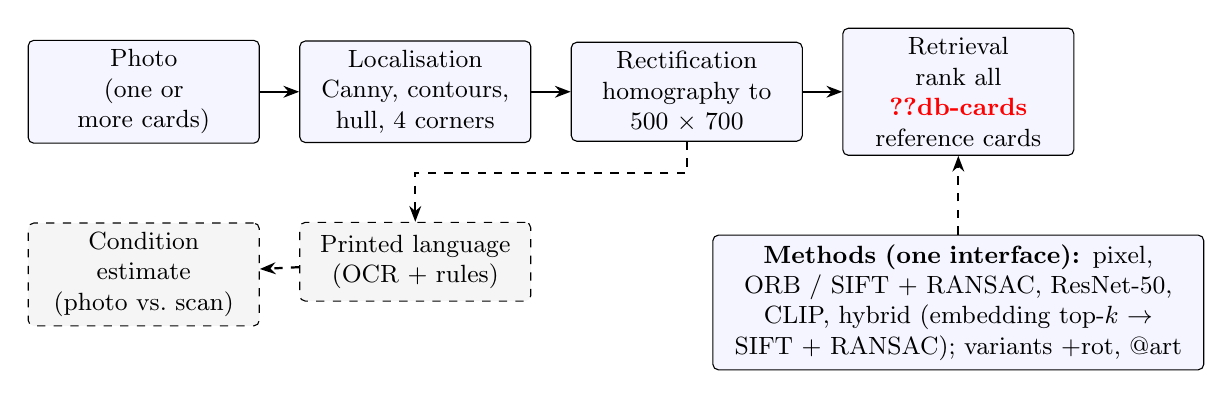
\begin{tikzpicture}[
    node distance=6mm and 5mm,
    box/.style={draw, rounded corners=2pt, align=center, font=\small, minimum height=10mm, text width=27mm, fill=blue!4},
    opt/.style={box, fill=gray!8, dashed},
    arr/.style={-{Stealth[length=2mm]}, thick}]
  \node[box] (photo) {Photo\\(one or more cards)};
  \node[box, right=of photo] (loc) {Localisation\\Canny, contours,\\hull, 4 corners};
  \node[box, right=of loc] (rect) {Rectification\\homography to\\$500\times700$};
  \node[box, right=of rect] (ret) {Retrieval\\rank all \res{db-cards}\\reference cards};
  \node[box, below=10mm of ret, text width=60mm] (methods) {\textbf{Methods (one interface):} pixel, ORB / SIFT + RANSAC, ResNet-50, CLIP, hybrid (embedding top-$k$ $\to$ SIFT + RANSAC); variants +rot, @art};
  \node[opt, below=10mm of loc] (lang) {Printed language\\(OCR + rules)};
  \node[opt, below=10mm of photo] (cond) {Condition estimate\\(photo vs.\ scan)};
  \draw[arr] (photo) -- (loc);
  \draw[arr] (loc) -- (rect);
  \draw[arr] (rect) -- (ret);
  \draw[arr, dashed] (methods) -- (ret);
  \draw[arr, dashed] (rect.south) |- ++(0,-4mm) -| (lang.north);
  \draw[arr, dashed] (lang) -- (cond);
\end{tikzpicture}
\caption[Pipeline overview]{Pipeline overview. Solid arrows: the identification pipeline that is evaluated in this report. Dashed boxes: extensions used by the application (Section~\ref{sec:extensions}).}
\label{fig:pipeline}
\end{figure}

\section{Card localisation}
\label{sec:localisation}

The detector (\texttt{cardrec/rectify.py}) is fully classical and has no learned parameters. Its design goal is to find the \emph{outer} outline of the card, not an inner frame such as the artwork box, under perspective, blur and glare.

\begin{enumerate}
  \item \textbf{Edge maps.} The photo is downscaled so that its longest side is at most 800 pixels and smoothed with a $5\times5$ Gaussian filter. Two channels are used: grey level and the HSV saturation, because a silver card border can have the same brightness as the table but a different colourfulness. On each channel the Canny detector \citep{canny1986edge} is run with three threshold pairs (fixed $50/150$, relative to the median grey level $0.5m/1.0m$, and low $10/40$ for blurry photos), and each edge map is dilated with a $3\times3$ kernel once (keeps the thin gap between touching cards) and twice (closes gaps in blurry edges). All twelve edge maps are used.
  \item \textbf{Candidate quadrilaterals.} Contours are extracted from every edge map \citep{suzuki1985contours}. For each contour, its convex hull is simplified with the Douglas--Peucker algorithm \citep{douglas1973peucker}, with a tolerance that grows from 2\% to 8\% of the perimeter until four corners remain. Using the hull instead of the raw contour makes the step robust to rounded card corners and to edges broken by glare.
  \item \textbf{Checks.} A quadrilateral is kept only if (i) its area is at least 3\% of the image, (ii) it does not touch the image border, (iii) its aspect ratio (long side / short side) is between 1.15 and 1.95 (a real card is $88/63\approx1.40$; perspective changes it), (iv) the contour fills at least 85\% of the quadrilateral, and (v) its four sides lie on real edges: of 60 points sampled along each side, at least 60\% must be edge pixels (``edge support''). The last check rejects large shapes stretched around background noise.
  \item \textbf{Selection.} Candidates are sorted by $\text{score} = \text{area}\times\text{support}^2$, so that a quadrilateral that also covers some background (lower support) loses to the true card outline. A candidate is dropped if its centre lies inside an already accepted card (inner frames) or if it overlaps one with intersection-over-union (IoU) above 0.5 (duplicates from different edge maps). Up to ten cards are returned.
\end{enumerate}

If no candidate passes, the single-card pipeline falls back to resizing the whole photo to $500\times700$. The thresholds were tuned only on separate development query sets, never on the test queries described in Chapter~\ref{ch:data}.

\section{Rectification}
\label{sec:rectification}

The four corners are ordered by their angle around the centroid and the list starts at the corner with the smallest $x+y$, which becomes the top-left corner of the output. If the top side is longer than the left side, the card is lying sideways and the order is rotated by one position. The perspective transform $H$ that maps the four corners $\mathbf{p}_i$ to the corners of the $500\times700$ rectangle $\mathbf{q}_i$ is computed exactly from the four correspondences,
\begin{equation}
  \lambda_i \begin{pmatrix} \mathbf{q}_i \\ 1 \end{pmatrix} = H \begin{pmatrix} \mathbf{p}_i \\ 1 \end{pmatrix}, \qquad i = 1,\dots,4,
  \label{eq:homography}
\end{equation}
and the photo is warped with $H$. This step cannot tell the top of the card from the bottom: a card rotated by $180^\circ$ produces a valid but upside-down rectification. With the corner ordering above, cards rotated by about $-45^\circ$ to $+135^\circ$ come out upright and other rotations come out upside down. Keypoint methods are rotation invariant and do not care; for the embedding methods, the ``+rot'' variant (Section~\ref{sec:variants}) addresses it.

\section{Retrieval interface}

Every method implements two operations: \texttt{build\_index(reference images, ids)}, run once, and \texttt{query(rectified card)}, which returns the \emph{complete} ranking of the database as (id, score) pairs. Reference scans are resized to the same $500\times700$ canonical size as the queries. Indexes are cached on disk, so the expensive index of the keypoint methods is computed only once.

\paragraph{Keypoint matching with RANSAC.} For SIFT \citep{lowe2004sift} and ORB \citep{rublee2011orb}, up to 800 keypoints are detected on the grey-level card. Each query descriptor is matched to its two nearest neighbours in a reference card by brute force (L2 distance for SIFT, Hamming distance for ORB), and a match is kept if it passes the ratio test with ratio 0.75. If at least four matches remain, a homography is estimated with RANSAC \citep{fischler1981ransac} using a reprojection threshold of 5 pixels, and the \emph{number of inliers} is the similarity score. The query is compared with every reference card.

\paragraph{Global embeddings.} An embedding method maps an image to a vector $\mathbf{f}$, normalised to unit length. The similarity between the query $\mathbf{f}_q$ and a reference $\mathbf{f}_r$ is the cosine similarity $s(q,r) = \mathbf{f}_q^\top\mathbf{f}_r$, computed for all references with one matrix product.

\section{Hybrid re-ranking}
\label{sec:hybrid}

The hybrid combines a fast embedding with precise geometric verification, in the spirit of spatial re-ranking \citep{philbin2007spatial}. Let $S_k$ be the $k$ references with the highest embedding similarity to the query. Only these $k$ cards are verified with SIFT + RANSAC, and they are re-ordered by
\begin{equation}
  \text{rank within } S_k \text{ by } \big(\, \text{inliers}(q,r) \downarrow,\;\; s(q,r) \downarrow \,\big),
  \label{eq:hybrid}
\end{equation}
that is, by the number of RANSAC inliers, with ties broken by the embedding similarity. The cards outside the shortlist keep their embedding order after the $k$ re-ranked cards, so the output is still a full ranking. The default shortlist size is $k=20$, so SIFT matching is done against 20 cards instead of \res{db-cards}. If the correct card is not in the shortlist, the hybrid cannot recover it; this is why the shortlist size is a parameter of the experiments.

\section{Variants}
\label{sec:variants}

\begin{itemize}
  \item \textbf{+rot} (embedding and hybrid methods only). The query is embedded twice, as rectified and rotated by $180^\circ$, and each reference keeps the higher of the two similarities. This removes the up/down ambiguity of the rectification at the cost of a second forward pass.
  \item \textbf{@art}. Both the references and the query are cropped to a fixed artwork window (rows 70--340, columns 35--465 of the $500\times700$ card) before indexing and querying. The window contains no text, so it is the same in every language. On full-art cards it is simply the upper-middle part of the illustration.
\end{itemize}

\section{Extensions used by the application}
\label{sec:extensions}

\paragraph{Printed language.} Identification and language are treated as separate problems. The card is identified from its image (for non-English cards, preferably with an @art method), and the printed language is classified separately (\texttt{cardrec/language.py}). The rectified card is re-warped at $750\times1050$ pixels, because the small text is unreadable at $500\times700$, and read by EasyOCR twice, once with a Japanese+English reader and once with a Spanish+English reader. Fixed rules then decide: (1) if kana characters (hiragana and katakana) make up at least 30\% of the letters read by the Japanese reader, the card is Japanese (kanji are not counted, because the reader invents kanji on blurry Latin text); (2) otherwise, the language code printed next to the set code at the bottom left (for example ``PRE EN'') is read in an enlarged crop; (3) otherwise, typical English and Spanish words and Spanish accented characters are counted, and the larger count wins; with no evidence the answer is ``unknown''.

\paragraph{Visual condition estimate.} Once a card is identified, its official scan is a picture of the undamaged card. The condition module (\texttt{cardrec/condition.py}) re-detects the outline precisely, warps the photo to $750\times1050$ pixels (about 12 pixels per millimetre), aligns the scan to the photo with SIFT + RANSAC and matches the colours. It then measures centering from the border widths, three sub-scores (whitening, fill, fray) for each of the four corners and four edges, and surface defects as remaining differences between photo and scan. These are combined into a 0--1000 score with hand-set weights. The result is explicitly labelled as an \emph{estimate}, not an official grade.

\paragraph{Application.} A local web application called CardDex (Flask back end, single-page front end, SQLite collection) puts the pipeline into practice (Figure~\ref{fig:app-screens}). The user uploads a photo and chooses one of eight retrieval methods (SIFT by default); a one-sentence description of each method, with its typical speed, is shown next to the selector, so that a user without a computer-vision background can choose, for example, the fast CLIP hybrid for everyday use or the artwork-only hybrid for non-English cards. The application detects and rectifies the card, ranks the reference cards with the selected method and shows the top-5 candidates with their scores, so that a wrong first guess can be corrected by clicking another candidate. For inlier-based methods it marks a result as a likely match when the best card has at least 15 inliers and at least 1.4 times the inliers of the second card. It then shows tags derived from the card metadata (set, number, name, category, stage, type, rarity, regulation mark, illustrator), classifies the printed language, optionally estimates the condition from a front and a back photo, and saves the card to a personal collection with its quantity, language and a market price (TCGdex first, Pok\'emon TCG API as fallback, cached for 24 hours). The collection panel can be filtered by every tag. Besides the \res{db-cards} English reference cards, the application's database contains the \res{db-ja-cards} cards of the Japanese set \emph{Battle Partners} (official scans from TCGdex), so that Japanese copies can be identified as Japanese cards and not only as their English counterparts. \res{db-ja-linked} of them were linked to the English card with the same artwork using the rule of the cross-language test set (Section~\ref{sec:langdata}), and all links were checked by eye. When the best match is a Japanese card, the application pre-selects Japanese as the language of the user's copy, and its price is taken from TCGdex's Japanese catalogue (Cardmarket, in EUR). These Japanese cards are used only by the application, not in the benchmark experiments of this report. The application is started with \texttt{run\_app.bat} or \texttt{python -m cardrec.app.server}; it runs locally and needs internet access only for prices.

\begin{figure}[htbp]
\centering
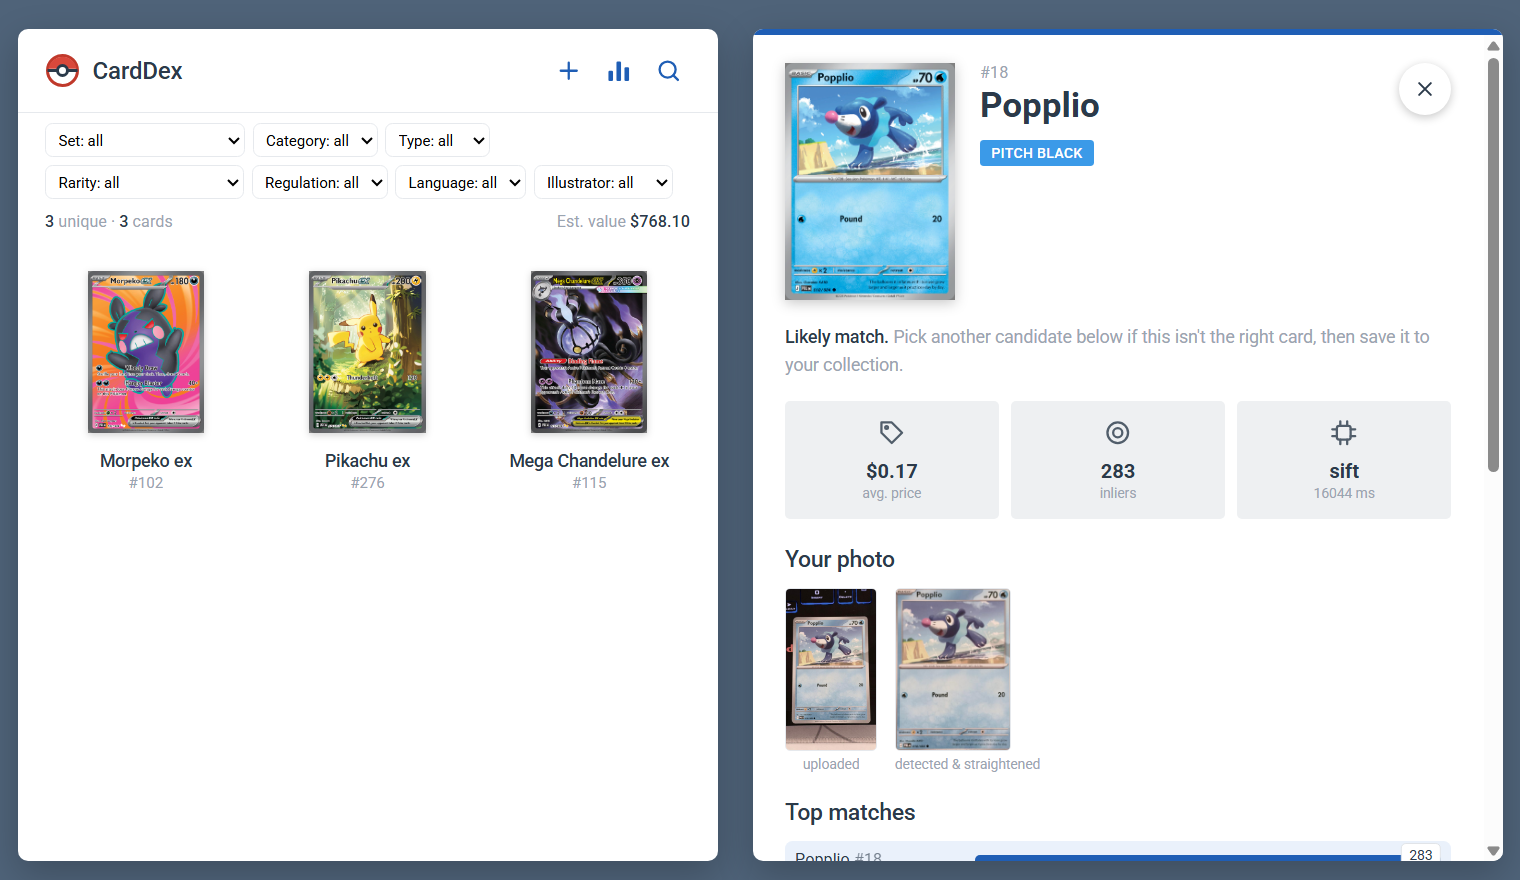
\includegraphics[width=\textwidth]{figures/app_analysis.png}\\[4pt]
\begin{subfigure}{0.49\textwidth}\centering
  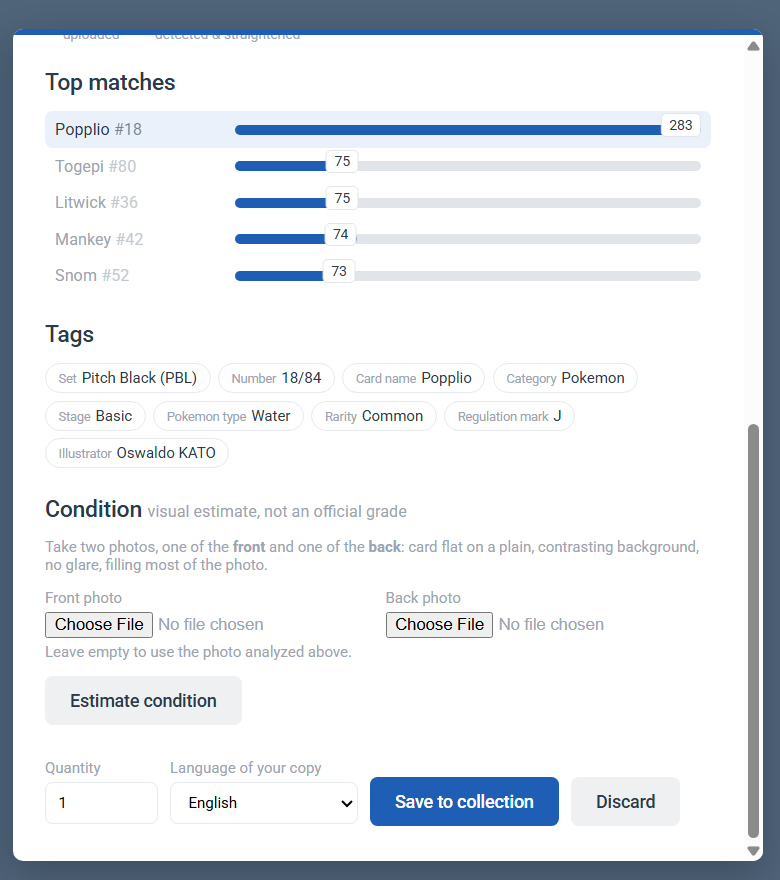
\includegraphics[width=\textwidth]{figures/app_matches_tags.png}
  \caption{Top-5 matches, tags and saving.}\label{fig:app-matches}
\end{subfigure}\hfill
\begin{subfigure}{0.49\textwidth}\centering
  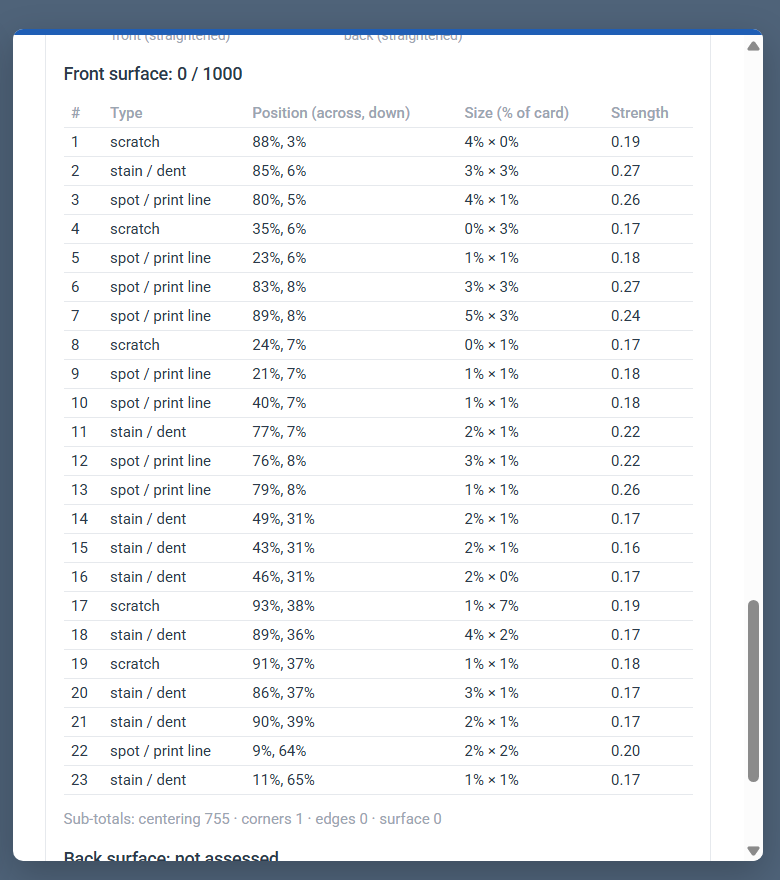
\includegraphics[width=\textwidth]{figures/app_surface.png}
  \caption{Condition report: surface table.}\label{fig:app-surface}
\end{subfigure}
\caption[The CardDex application]{The CardDex application (screenshots by the author on 1 November 2026, browser frame removed; the collection shown is the one at that date). Top: collection with tag filters (left) and the analysis of an uploaded phone photo (right): best match, average price, number of RANSAC inliers, method and time, and the uploaded and straightened photo. (a) The ranked candidates, the tags taken from the database and the save form. (b) Part of the condition report of the same card.}
\label{fig:app-screens}
\end{figure}
  % Technical approach
\chapter{Dataset and Experimental Setup}
\label{ch:data}

%-------------------------------------------------------

\section{Reference database}

The reference database contains one official scan per card for \res{db-sets} recent sets of the Pok\'emon Trading Card Game (Table~\ref{tab:dataset}): \res{db-cards} unique card ids in total, of which \res{db-pokemon} are Pok\'emon cards, \res{db-trainer} Trainer cards and \res{db-energy} Energy cards. The counts include the secret rares, which are numbered above the printed set size. Card lists, metadata and images come from the Pok\'emon TCG API; illustrator names missing in that source and the Spanish and Japanese scans used in the language test come from TCGdex. The download script (\texttt{cardrec/database.py}) writes a manifest with one row per card (id, name, set, number, supertype, subtypes, types, rarity, regulation mark, illustrator, image path, artwork group).

\begin{table}[htbp]\centering\small
\caption[Reference database]{Reference database: one official scan per card id. ``Printed'' is the set size printed on the cards; the extra cards are secret rares numbered above it.}\label{tab:dataset}
\begin{tabular}{@{}llrr@{}}
\toprule
Set (API id) & Code & Cards & Printed\\
\midrule
Prismatic Evolutions (\texttt{sv8pt5}) & PRE & 180 & 131\\
Journey Together (\texttt{sv9}) & JTG & 190 & 159\\
Ascended Heroes (\texttt{me2pt5}) & ASC & 295 & 217\\
Pitch Black (\texttt{me5}) & PBL & 120 & 84\\
\midrule
Total & & 785 & 591\\
\bottomrule
\end{tabular}
\end{table}


\section{Reprints and near-duplicates}
\label{sec:reprints}

Two kinds of near-duplicates are handled differently.

\paragraph{Identical artwork (reprints).} Some cards are reprinted in a later set with exactly the same artwork; only the small set symbol, set code and collector number differ. Such pairs are grouped automatically (\texttt{cardrec/art\_groups.py}) with a 64-bit perceptual hash: the grey card is resized to $32\times32$, transformed with the discrete cosine transform, and the $8\times8$ lowest-frequency coefficients are thresholded at their median, giving one bit each. Two cards are considered the same artwork if \emph{both} the hash of the whole card and the hash of the artwork window differ in at most 6 bits (Hamming distance). Groups are then formed transitively with union--find. This produced \res{db-art-pairs} same-artwork pairs, all between \emph{Ascended Heroes} and an older set (\res{db-art-pairs-sv8pt5-me2pt5} with \emph{Prismatic Evolutions} and \res{db-art-pairs-sv9-me2pt5} with \emph{Journey Together}), so the \res{db-cards} cards contain \res{db-artgroups} distinct artworks. The largest distances inside accepted pairs were \res{db-art-maxfull} bits (whole card) and \res{db-art-maxart} bits (artwork window). All pairs were checked by eye on a generated contact sheet.

\paragraph{Lookalikes.} Cards with the same name but different artwork (for example the \res{db-max-name-n} versions of \emph{\res{db-max-name}}, or a regular card and its illustration rare) are \emph{not} grouped: they are different cards that a correct system must tell apart. The database has \res{db-dup-names} names that occur on more than one card (\res{db-dup-name-cards} cards).

\paragraph{Metrics that follow from this.} Every query is scored twice:
\begin{itemize}
  \item \textbf{strict}: correct only if the predicted id is exactly the true id;
  \item \textbf{lenient}: correct if the predicted card is in the same artwork group as the true card (a reprint counts as correct).
\end{itemize}
The difference between the two metrics measures exactly how many errors are reprint confusions.

\section{Synthetic test queries}
\label{sec:synthetic}

Real labelled photos of all \res{db-cards} cards do not exist, so the main experiments use synthetic photos with exact ground truth (\texttt{cardrec/synth.py}). A reference scan is placed on a $1280\times960$ background (a random smooth colour field plus noise) with a random position, in-plane rotation and a random perturbation of its four corners (perspective). The whole image then receives a lighting gradient with a gamma change, a glare blob centred on the card, Gaussian or motion blur, and Gaussian noise, and is saved as JPEG (quality 92). The strength of each distortion is set by a severity level from 1 to 5 (Table~\ref{tab:severity}); at severity 5 the rotation covers the full circle. The true corner positions are stored with each query, so the accuracy of the detector can be measured as well.

\begin{table}[htbp]\centering\small
\caption[Synthetic distortion severities]{Distortion parameters per severity level (\texttt{cardrec/synth.py}). Each value is the maximum of a random draw.}\label{tab:severity}
\begin{tabular}{@{}lccccc@{}}
\toprule
Parameter & S1 & S2 & S3 & S4 & S5\\
\midrule
Max.\ in-plane rotation ($\pm$deg) & 5 & 15 & 30 & 60 & 180\\
Corner jitter (frac.\ of card height) & 0.02 & 0.04 & 0.07 & 0.1 & 0.14\\
Blur $\sigma$ (px, Gaussian or motion) & 0 & 1 & 1.8 & 2.8 & 4\\
Gaussian noise $\sigma$ (grey levels) & 2 & 5 & 8 & 12 & 18\\
Lighting gradient + gamma strength & 0.1 & 0.2 & 0.3 & 0.4 & 0.5\\
Glare blob strength & 0 & 0.2 & 0.4 & 0.6 & 0.8\\
\bottomrule
\end{tabular}
\end{table}


For each severity, \res{main-n-queries} different cards are drawn at random without replacement (fixed seed), so each test set covers about a quarter of the database. Note that the cards differ between severities, so a comparison across severities also involves different cards. Separate development query sets with other seeds were used to tune the detector; the test queries were never used for tuning.

\section{Cross-language test set}
\label{sec:langdata}

To test printed languages, a separate set was built from official scans (\texttt{cardrec/lang\_data.py}) with two disjoint splits, a development split for tuning the language rules and a test split for the reported numbers. The test split has 60 English cards from the database, 60 Spanish cards (same card ids as their English versions) and 60 Japanese cards from the two Japanese sets that correspond to \emph{Prismatic Evolutions} and \emph{Journey Together}. Japanese numbering differs, so the matching English card was found \emph{without} the tested methods: same illustrator and same Pok\'edex number, then the closest artwork hash, accepted only up to a distance of 14 bits. This gave an English ground truth for \res{lang-ja-n} of the 60 Japanese cards; all matches were checked by eye, and the remaining Japanese cards are used only for language classification. Synthetic photos were rendered at severity 2 at two resolutions: the standard canvas (card about 530 pixels tall, ``low'') and a $2560\times1920$ canvas (card about 1050 pixels tall, similar to a 12-megapixel phone photo, ``phone'').

\section{Condition validation set}

The condition estimate was tuned on \res{cond-dev-n} development cards and is validated on \res{cond-n} test cards drawn with a different random seed (the two samples were not forced to be disjoint: \res{cond-dev-overlap} cards appear in both, with different random damage). Each official scan is damaged with known strengths in $\{0, 0.25, 0.5, 0.75, 1\}$: corner whitening, corner cuts, edge whitening, edge fraying, scratches and stains at known positions, and a shift of the print of up to about 1\,mm (centering). The damaged card is rendered as a phone-resolution photo at severity 1 and analysed exactly like a real photo. Only the front side can be validated, because no official scans of the card back exist.

\section{Metrics}

\begin{itemize}
  \item \textbf{Top-1 / top-5}: fraction of queries whose correct card is ranked first / among the first five.
  \item \textbf{MRR}: mean reciprocal rank $\frac{1}{N}\sum_i 1/\text{rank}_i$. With exactly one relevant card per query, mean average precision equals the MRR.
  \item \textbf{95\% confidence intervals}: percentile bootstrap \citep{efron1979bootstrap} over the queries, 1000 resamples.
  \item \textbf{Outline accuracy}: IoU between the detected and the true card polygons; a rectification counts as correct if IoU $\geq 0.8$, and as a localisation failure if IoU $< 0.5$.
  \item \textbf{Latency}: median time per photo for rectification plus retrieval. The experiments ran on a laptop that was running other jobs (including other experiments) at the same time, so the latencies indicate orders of magnitude, not exact times; accuracy is not affected.
\end{itemize}
Every query of every run is logged (predicted id, rank of the true card, outline IoU, timings), and all tables and figures of this report are regenerated from these logs by a script (\texttt{report/make\_figures.py}).

\section{Real photos}
\label{sec:realphotos}

A protocol and labelling tools for real phone photos are ready (\texttt{cardrec/real\_photos.py}): 70--100 photos per set of physically owned cards, with deliberately varied backgrounds, lighting, glare, sleeves, rotation, and 20--30 photos with several cards; the ground truth must be entered by hand and not taken from any tested method. This systematic set was not collected within the project. The real photos used in this report are the \res{app-reid-n} photos that were saved with the identified cards in the application (Section~\ref{sec:res-app}); for these, the ground truth is the card that the author confirmed in the application before saving.
  % Dataset and experimental setup
\chapter{Baseline and Comparison Methods}
\label{ch:methods}

%-------------------------------------------------------

All methods receive the same rectified $500\times700$ card and return a full ranking of the \res{db-cards} reference cards. Table~\ref{tab:methods} lists them with the settings used in the code. No method is trained or fine-tuned on card data; the deep models are used frozen with their public pretrained weights.

\begin{table}[htbp]\centering\small
\caption[Compared methods]{Compared retrieval methods and their settings as implemented (\texttt{cardrec/methods/}).}
\label{tab:methods}
\begin{tabular}{@{}P{1.45in}P{2.6in}P{1.85in}@{}}
\toprule
Method & Representation & Similarity \\
\midrule
Pixel thumbnail (sanity baseline) & $32\times44$ grey thumbnail, mean subtracted ($1408$-d) & cosine \\
ORB + RANSAC & up to 800 ORB keypoints, binary descriptors & ratio test 0.75, RANSAC homography inliers (5\,px), against every card \\
SIFT + RANSAC & up to 800 SIFT keypoints, 128-d descriptors & as ORB, with L2 distance \\
ResNet-50 & ImageNet ResNet-50, classification layer removed, global average pooled 2048-d vector; input: whole card resized to $224\times320$ & cosine \\
CLIP ViT-B/32 & CLIP image encoder, 512-d image embedding; default preprocessing (short side to 224, centre crop $224\times224$) & cosine \\
Hybrid ResNet$\to$SIFT, Hybrid CLIP$\to$SIFT & top-$k$ shortlist from the embedding ($k=20$ by default) & SIFT + RANSAC inliers inside the shortlist, ties by cosine \\
\midrule
+rot (embedding methods) & also embed the query rotated $180^\circ$ & best of the two \\
@art (any method) & only the artwork window of query and references & as the base method \\
\bottomrule
\end{tabular}
\end{table}

\section{Why these methods}

\paragraph{Pixel thumbnail.} A deliberately weak baseline. If the pipeline only had to undo a perfect warp of the reference image, comparing tiny thumbnails would already work; its accuracy therefore shows how easy the synthetic queries are once the card is rectified, and it gives a lower bound for the other methods.

\paragraph{ORB and SIFT with RANSAC.} The classical approach to instance recognition of flat objects \citep{lowe2004sift, rublee2011orb, fischler1981ransac}. They are rotation invariant, use fine details (the collector number, the set symbol) as well as the artwork, and verify geometric consistency, which makes them precise. Their cost grows linearly with the database because every reference card is matched; ORB is the cheaper binary variant.

\paragraph{ResNet-50.} A convolutional network pretrained on ImageNet \citep{he2016resnet, deng2009imagenet}, used as an off-the-shelf global descriptor \citep{razavian2014cnnfeatures, babenko2014neuralcodes}. It sees the whole card with its 5:7 shape.

\paragraph{CLIP ViT-B/32.} The image encoder of CLIP \citep{radford2021clip}, a vision transformer \citep{dosovitskiy2021vit} trained on image--text pairs. Its default preprocessing crops the centre square of the card, so the top and bottom of the card (about one seventh each, including the name bar and the collector number) are not seen. This is the preprocessing of the released model and was kept on purpose, but it is a limitation for telling card versions apart.

\paragraph{Hybrids.} The embedding chooses $k$ candidates, and SIFT + RANSAC decides among them (Section~\ref{sec:hybrid}). The expected benefit is SIFT-level precision at a fraction of its cost, as long as the correct card is in the shortlist.

\section{Experiments}

The experiment script (\texttt{cardrec/experiments.py}) defines four comparisons:
\begin{enumerate}
  \item \textbf{main}: the eleven configurations of Table~\ref{tab:main} (pixel, ORB, SIFT, ResNet-50, CLIP, both hybrids, and the +rot variants of the last four) at all five severities, \res{main-n-queries} queries each;
  \item \textbf{k-sweep}: both hybrids with $k\in\{5, 10, 20, 50\}$ at severity 3, accuracy versus latency;
  \item \textbf{no-rectify ablation}: every configuration at severity 3 with the whole photo resized instead of rectified;
  \item \textbf{scenes}: multi-card scenes with 2--6 cards and maximum overlaps of 0\%, 15\% and 30\%, evaluated with ResNet-50, CLIP and both hybrids.
\end{enumerate}
All four are produced by \texttt{python -m cardrec.experiments --exp all}; each run logs every query, so all tables and figures of Chapter~\ref{ch:results} are regenerated from the logs by \texttt{report/make\_figures.py}.
  % Baseline and comparison methods
\chapter{Results}
\label{ch:results}

%-------------------------------------------------------

This chapter reports the results of all experiments. All accuracies are on the synthetic test queries unless stated otherwise; real photos are covered in Section~\ref{sec:res-app}.

\section{Localisation and rectification}
\label{sec:res-rect}

The detector is the same for every retrieval method, so its accuracy on the test queries is a property of the query set. Figure~\ref{fig:pipeline-example} shows a typical successful case. On the \res{main-n-queries} single-card test queries per severity, the detected outline was correct (IoU $\geq 0.8$) for \res{rect-s1-ok}\%, \res{rect-s2-ok}\%, \res{rect-s3-ok}\%, \res{rect-s4-ok}\% and \res{rect-s5-ok}\% of the queries at severities 1 to 5. At severities 4 and 5 the detector returned a card outline at all for only \res{rect-s4-found}\% and \res{rect-s5-found}\% of the queries; in the remaining cases the pipeline fell back to the whole photo.

\begin{figure}[htbp]\centering
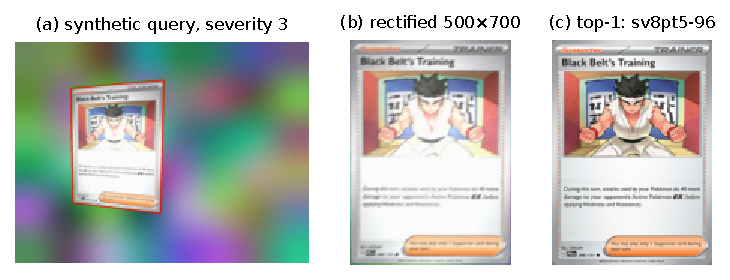
\includegraphics[width=\textwidth]{figures/pipeline_example.pdf}
\caption[Pipeline example]{Example run of the pipeline. (a) Synthetic query \texttt{s3\_0000}; green = true outline, red = outline found by the detector. (b) The card warped to the canonical view. (c) The reference scan ranked first by ORB + RANSAC (correct; 145 RANSAC inliers versus 67 for the second card).}\label{fig:pipeline-example}
\end{figure}


\section{Single-card identification (main comparison)}
\label{sec:res-main}

Table~\ref{tab:main} and Figure~\ref{fig:severity} show the strict and lenient top-1 accuracy of every method at every severity; Table~\ref{tab:main-detail} in Appendix~\ref{app:repro} adds top-5, MRR, 95\% confidence intervals and latencies.

\begin{table}[htbp]\centering\footnotesize
\caption[Top-1 accuracy per method and severity]{Top-1 identification accuracy on the synthetic single-card test queries (200 per severity), shown as strict / lenient. Strict = exact card id; lenient = any card with the same artwork (reprint). 95\% bootstrap intervals are in Table~\ref{tab:main-detail} and Figure~\ref{fig:severity}.}
\label{tab:main}
\begin{tabular}{@{}lccccc@{}}
\toprule
Method & S1 & S2 & S3 & S4 & S5\\
\midrule
Pixel thumbnail & 0.970 / 0.980 & 0.930 / 0.950 & 0.900 / 0.930 & 0.600 / 0.615 & 0.065 / 0.070\\
\midrule
ORB + RANSAC & 0.995 / 1.000 & 0.975 / 1.000 & 0.970 / 0.995 & 0.725 / 0.740 & 0.085 / 0.085\\
SIFT + RANSAC & 0.995 / 1.000 & 0.970 / 1.000 & 0.930 / 0.950 & 0.745 / 0.765 & 0.110 / 0.125\\
ResNet-50 & 0.970 / 0.995 & 0.780 / 0.800 & 0.375 / 0.380 & 0.120 / 0.120 & 0.025 / 0.025\\
CLIP ViT-B/32 & 0.970 / 1.000 & 0.955 / 0.995 & 0.845 / 0.875 & 0.250 / 0.255 & 0.020 / 0.020\\
Hybrid ResNet$\to$SIFT & 0.995 / 1.000 & 0.940 / 0.970 & 0.755 / 0.780 & 0.370 / 0.385 & 0.050 / 0.050\\
Hybrid CLIP$\to$SIFT & 0.995 / 1.000 & 0.965 / 0.995 & 0.935 / 0.955 & 0.530 / 0.535 & 0.020 / 0.020\\
ResNet-50 +rot & 0.970 / 0.995 & 0.745 / 0.760 & 0.340 / 0.345 & 0.130 / 0.130 & 0.030 / 0.030\\
CLIP +rot & 0.970 / 1.000 & 0.950 / 0.990 & 0.810 / 0.840 & 0.275 / 0.280 & 0.020 / 0.020\\
Hybrid ResNet$\to$SIFT +rot & 0.995 / 1.000 & 0.940 / 0.970 & 0.715 / 0.735 & 0.370 / 0.375 & 0.055 / 0.055\\
Hybrid CLIP$\to$SIFT +rot & 0.995 / 1.000 & 0.965 / 0.995 & 0.925 / 0.945 & 0.565 / 0.570 & 0.040 / 0.040\\
\bottomrule
\end{tabular}
\end{table}

\begin{figure}[htbp]\centering
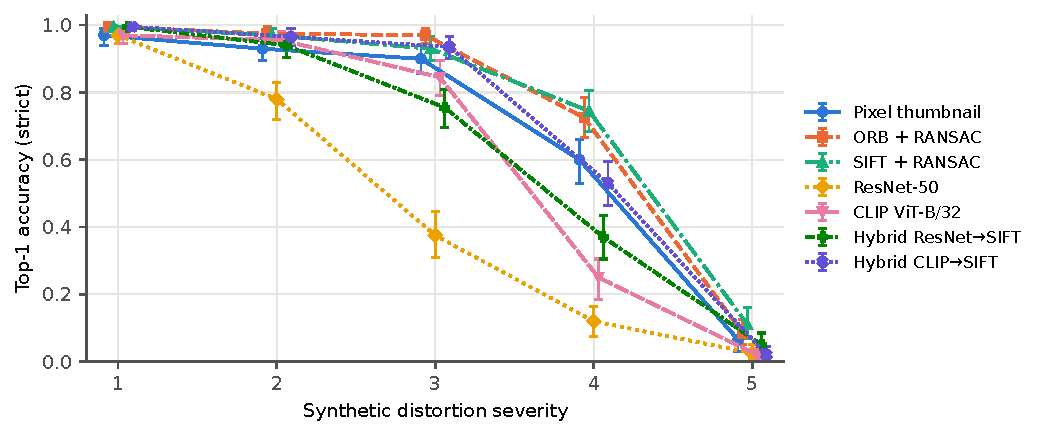
\includegraphics[width=\textwidth]{figures/accuracy_vs_severity.pdf}
\caption[Accuracy versus distortion severity]{Strict top-1 accuracy versus synthetic distortion severity for the seven base methods, with 95\% bootstrap intervals (200 queries per point; points slightly shifted horizontally for readability; the +rot variants are in Table~\ref{tab:main}).}\label{fig:severity}
\end{figure}


\paragraph{Mild distortion (severities 1--2).} All methods except ResNet-50 were close to perfect. At severity 1, ORB, SIFT and both hybrids reached a strict top-1 of \res{orb-s1-top1}, \res{sift-s1-top1}, \res{hybrid_resnet_k20-s1-top1} and \res{hybrid_clip_k20-s1-top1}, and ResNet-50 and CLIP \res{resnet-s1-top1} and \res{clip-s1-top1}. At severity 2 ResNet-50 already dropped to \res{resnet-s2-top1}, while CLIP kept \res{clip-s2-top1} and the CLIP hybrid \res{hybrid_clip_k20-s2-top1}. Under the lenient metric, ORB reached \res{orb-s1-top1_len} and \res{orb-s2-top1_len} and SIFT \res{sift-s1-top1_len} and \res{sift-s2-top1_len}, so every strict error of ORB and SIFT at these severities was a confusion with a reprint of the same artwork.

\paragraph{Moderate distortion (severity 3).} The methods separate clearly. ORB + RANSAC reached \res{orb-s3-top1} {\small[\res{orb-s3-top1_lo}, \res{orb-s3-top1_hi}]}, SIFT + RANSAC \res{sift-s3-top1} {\small[\res{sift-s3-top1_lo}, \res{sift-s3-top1_hi}]}, the CLIP hybrid \res{hybrid_clip_k20-s3-top1} {\small[\res{hybrid_clip_k20-s3-top1_lo}, \res{hybrid_clip_k20-s3-top1_hi}]}, CLIP alone \res{clip-s3-top1}, the ResNet hybrid \res{hybrid_resnet_k20-s3-top1} and ResNet-50 alone only \res{resnet-s3-top1}. Re-ranking the shortlist with SIFT therefore raised CLIP from \res{clip-s3-top1} to \res{hybrid_clip_k20-s3-top1} and ResNet-50 from \res{resnet-s3-top1} to \res{hybrid_resnet_k20-s3-top1}. The pixel-thumbnail baseline reached \res{pixel-s3-top1}, more than both global deep embeddings alone; this is discussed in Section~\ref{sec:disc-synthetic}.

\paragraph{Strong distortion (severities 4--5).} At severity 4, the two exhaustive keypoint methods remained best, SIFT with \res{sift-s4-top1} {\small[\res{sift-s4-top1_lo}, \res{sift-s4-top1_hi}]} and ORB with \res{orb-s4-top1} {\small[\res{orb-s4-top1_lo}, \res{orb-s4-top1_hi}]} (overlapping intervals), followed by the pixel baseline (\res{pixel-s4-top1}), the CLIP hybrid with rotation (\res{hybrid_clip+rot_k20-s4-top1}) and without (\res{hybrid_clip_k20-s4-top1}), the ResNet hybrid (\res{hybrid_resnet_k20-s4-top1}), CLIP (\res{clip-s4-top1}) and ResNet-50 (\res{resnet-s4-top1}). At severity 5 every method failed (strict top-1 between \res{clip-s5-top1} for CLIP and \res{sift-s5-top1} for SIFT), because the card outline was found correctly in only \res{rect-s5-ok}\% of these photos (Section~\ref{sec:failures}).

\paragraph{Trying both orientations (+rot).} Embedding the query also rotated by $180^\circ$ removed every ``upside down'' failure (Table~\ref{tab:failures}), but it did not improve the accuracy: at severity 3 it was slightly lower for every embedding method (for example CLIP \res{clip+rot-s3-top1} versus \res{clip-s3-top1}, CLIP hybrid \res{hybrid_clip+rot_k20-s3-top1} versus \res{hybrid_clip_k20-s3-top1}), and at severity 4 slightly higher for CLIP and its hybrid (\res{clip+rot-s4-top1} versus \res{clip-s4-top1}, \res{hybrid_clip+rot_k20-s4-top1} versus \res{hybrid_clip_k20-s4-top1}); in every case the 95\% intervals of the two variants overlap. A plausible explanation is that comparing each reference with two versions of the query also doubles the chances of a wrong card scoring high. In the failure analysis, pooled over all severities, the number of failures with and without +rot was \res{fail-resnet+rot-total} versus \res{fail-resnet-total} for ResNet-50, \res{fail-clip+rot-total} versus \res{fail-clip-total} for CLIP, \res{fail-hybrid_resnet+rot_k20-total} versus \res{fail-hybrid_resnet_k20-total} for the ResNet hybrid and \res{fail-hybrid_clip+rot_k20-total} versus \res{fail-hybrid_clip_k20-total} for the CLIP hybrid: the upside-down failures disappear, but other failures take most of their place.

\paragraph{ORB versus SIFT.} The two keypoint methods were statistically tied at every severity: ORB was slightly ahead at severity 3 (\res{orb-s3-top1} versus \res{sift-s3-top1}) and SIFT slightly ahead at severities 4 and 5 (\res{sift-s4-top1} versus \res{orb-s4-top1}, \res{sift-s5-top1} versus \res{orb-s5-top1}), with overlapping 95\% intervals in every case. Both match the query against all \res{db-cards} reference cards, which took several seconds per photo on the test laptop (median \res{orb-s3-ms}~ms for ORB and \res{sift-s3-ms}~ms for SIFT at severity 3).

\section{Shortlist size of the hybrid}
\label{sec:res-ksweep}

Figure~\ref{fig:ksweep} shows how the shortlist size $k$ trades accuracy for time at severity 3. For the CLIP hybrid the shortlist matters little: strict top-1 grew from \res{ks-clip-k5-top1} with $k=5$ (median \res{ks-clip-k5-ms}~ms per photo) to \res{ks-clip-k20-top1} with $k=20$ (\res{ks-clip-k20-ms}~ms) and \res{ks-clip-k50-top1} with $k=50$ (\res{ks-clip-k50-ms}~ms). Already with $k=20$ the hybrid matched exhaustive SIFT (\res{sift-s3-top1}, median \res{sift-s3-ms}~ms per photo), which uses exactly the same SIFT verification but against all \res{db-cards} cards instead of 20; with $k=50$ its 95\% interval {\small[\res{ks-clip-k50-top1_lo}, \res{ks-clip-k50-top1_hi}]} also overlaps that of exhaustive ORB (\res{orb-s3-top1} {\small[\res{orb-s3-top1_lo}, \res{orb-s3-top1_hi}]}, median \res{orb-s3-ms}~ms), in a fraction of the time. For the ResNet hybrid the shortlist is decisive: \res{ks-resnet-k5-top1} with $k=5$, \res{ks-resnet-k20-top1} with $k=20$ and \res{ks-resnet-k50-top1} with $k=50$, because ResNet-50 often does not rank the correct card among its first few candidates, and SIFT can only choose among the cards it is given.

\begin{figure}[htbp]\centering
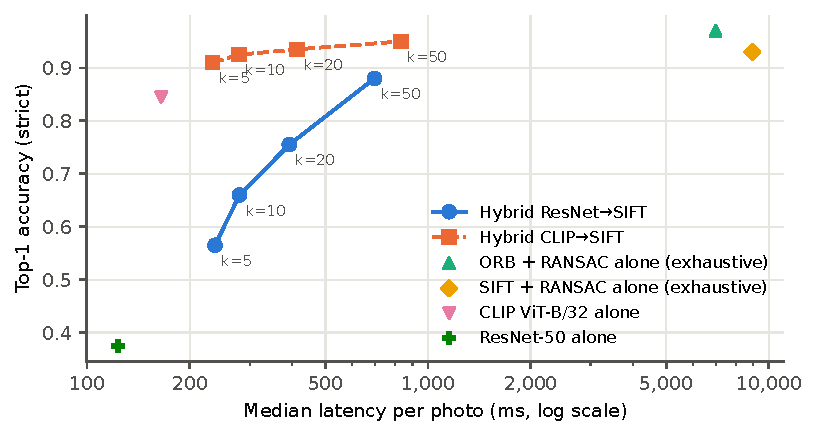
\includegraphics[width=\textwidth]{figures/ksweep.pdf}
\caption{Hybrid shortlist size $k$ (5, 10, 20, 50) at severity 3: accuracy versus median latency, compared with each component alone.}\label{fig:ksweep}
\end{figure}


\section{Effect of rectification}
\label{sec:res-norect}

Table~\ref{tab:norectify} compares each method at severity 3 with and without the rectification step. Without it, the global methods collapsed: the CLIP hybrid fell from \res{hybrid_clip_k20-s3-top1} to \res{norect-hybrid_clip_k20-top1}, CLIP from \res{clip-s3-top1} to \res{norect-clip-top1}, ResNet-50 from \res{resnet-s3-top1} to \res{norect-resnet-top1} and the pixel baseline from \res{pixel-s3-top1} to \res{norect-pixel-top1}. In these photos the card covers only part of the image and is rotated and seen in perspective; resizing the whole photo leaves most of the image as background, which dominates a global descriptor. The keypoint methods degraded less: SIFT kept \res{norect-sift-top1} (from \res{sift-s3-top1}) and ORB \res{norect-orb-top1} (from \res{orb-s3-top1}). Their features are local and invariant to rotation and scale, and the RANSAC homography can itself absorb the perspective, so they do not need the card to fill the image; they still lose most of their accuracy, because the small, unrectified card provides far fewer keypoints. Rectification is therefore a necessary step for every method, and essential for the global ones.

\begin{table}[htbp]\centering\small
\caption[Rectification ablation]{Ablation at severity 3: strict top-1 with rectification versus the whole photo resized to the canonical size.}\label{tab:norectify}
\begin{tabular}{@{}lcc@{}}
\toprule
Method & Rectified & Whole photo\\
\midrule
Pixel thumbnail & 0.900 & 0.005\\
ORB + RANSAC & 0.970 & 0.165\\
SIFT + RANSAC & 0.930 & 0.425\\
ResNet-50 & 0.375 & 0.005\\
CLIP ViT-B/32 & 0.845 & 0.020\\
Hybrid ResNet$\to$SIFT & 0.755 & 0.090\\
Hybrid CLIP$\to$SIFT & 0.935 & 0.080\\
ResNet-50 +rot & 0.340 & 0.005\\
CLIP +rot & 0.810 & 0.025\\
Hybrid ResNet$\to$SIFT +rot & 0.715 & 0.100\\
Hybrid CLIP$\to$SIFT +rot & 0.925 & 0.075\\
\bottomrule
\end{tabular}
\end{table}


\section{Multi-card scenes}
\label{sec:res-scenes}

Table~\ref{tab:scenes} reports the scenes with 2--6 cards at severity 2. Detection is the same for every method. With no overlap the detector found \res{sc-o0-recall} of the cards with a precision of \res{sc-o0-precision}; with up to 15\% and 30\% overlap, recall fell to \res{sc-o15-recall} and \res{sc-o30-recall}. The best end-to-end result (card detected \emph{and} correctly identified) was obtained by the CLIP hybrid: \res{sc-hybrid_clip_k20-o0-e2e_top1} without overlap, \res{sc-hybrid_clip_k20-o15-e2e_top1} and \res{sc-hybrid_clip_k20-o30-e2e_top1} with overlap. Among the cards that were detected, the CLIP hybrid identified \res{sc-hybrid_clip_k20-o0-id_acc_given_detected} correctly without overlap, so the loss comes mostly from detection: overlapping cards merge into one contour, as expected from the design of the detector (Section~\ref{sec:localisation}).

\begin{table}[htbp]\centering\small
\caption[Multi-card scenes]{Multi-card synthetic scenes (severity 2): detection precision / recall / F1 (IoU $\geq$ 0.5) and end-to-end top-1 (detected and correctly identified / all cards).}\label{tab:scenes}
\begin{tabular}{@{}lccccc@{}}
\toprule
Method & Overlap & P & R & F1 & End-to-end top-1\\
\midrule
ResNet-50 & 0\% & 0.911 & 0.706 & 0.795 & 0.349 {\scriptsize[0.30, 0.40]}\\
ResNet-50 & 15\% & 0.759 & 0.330 & 0.460 & 0.168 {\scriptsize[0.13, 0.20]}\\
ResNet-50 & 30\% & 0.721 & 0.291 & 0.415 & 0.154 {\scriptsize[0.12, 0.19]}\\
CLIP ViT-B/32 & 0\% & 0.911 & 0.706 & 0.795 & 0.571 {\scriptsize[0.52, 0.62]}\\
CLIP ViT-B/32 & 15\% & 0.759 & 0.330 & 0.460 & 0.267 {\scriptsize[0.22, 0.31]}\\
CLIP ViT-B/32 & 30\% & 0.721 & 0.291 & 0.415 & 0.220 {\scriptsize[0.18, 0.26]}\\
Hybrid ResNet$\to$SIFT & 0\% & 0.911 & 0.706 & 0.795 & 0.574 {\scriptsize[0.53, 0.63]}\\
Hybrid ResNet$\to$SIFT & 15\% & 0.759 & 0.330 & 0.460 & 0.275 {\scriptsize[0.23, 0.32]}\\
Hybrid ResNet$\to$SIFT & 30\% & 0.721 & 0.291 & 0.415 & 0.240 {\scriptsize[0.20, 0.28]}\\
Hybrid CLIP$\to$SIFT & 0\% & 0.911 & 0.706 & 0.795 & 0.643 {\scriptsize[0.59, 0.69]}\\
Hybrid CLIP$\to$SIFT & 15\% & 0.759 & 0.330 & 0.460 & 0.285 {\scriptsize[0.24, 0.33]}\\
Hybrid CLIP$\to$SIFT & 30\% & 0.721 & 0.291 & 0.415 & 0.247 {\scriptsize[0.21, 0.29]}\\
\bottomrule
\end{tabular}
\end{table}


\section{Identification across printed languages}
\label{sec:res-language-id}

In this experiment SIFT, CLIP and the CLIP hybrid were run on the same English, Spanish and Japanese queries (Table~\ref{tab:language-id}). All queries are at severity 2, so the in-plane rotation is at most $15^\circ$ and the upside-down problem does not occur.

\begin{table}[htbp]\centering\footnotesize
\caption[Identification per printed language]{Lenient top-1 identification per printed language (test split, severity 2) with 95\% bootstrap intervals, at two photo resolutions: card about 530~px tall (``low'') and about 1050~px tall (``phone'', like a 12~MP photo). @art = only the artwork window is compared; +rot = the query is also tried rotated 180\textdegree. Queries: en 60, es 60, ja 43.}\label{tab:language-id}
\begin{tabular}{@{}lllll@{}}
\toprule
Method & Res. & English & Spanish & Japanese\\
\midrule
SIFT + RANSAC & low & 1.000 {\scriptsize[1.00, 1.00]} & 1.000 {\scriptsize[1.00, 1.00]} & 1.000 {\scriptsize[1.00, 1.00]}\\
 & phone & 1.000 {\scriptsize[1.00, 1.00]} & 1.000 {\scriptsize[1.00, 1.00]} & 0.977 {\scriptsize[0.93, 1.00]}\\
\addlinespace[2pt]
SIFT + RANSAC @art & low & 1.000 {\scriptsize[1.00, 1.00]} & 1.000 {\scriptsize[1.00, 1.00]} & 1.000 {\scriptsize[1.00, 1.00]}\\
 & phone & 1.000 {\scriptsize[1.00, 1.00]} & 1.000 {\scriptsize[1.00, 1.00]} & 1.000 {\scriptsize[1.00, 1.00]}\\
\addlinespace[2pt]
CLIP ViT-B/32 & low & 0.983 {\scriptsize[0.95, 1.00]} & 0.883 {\scriptsize[0.80, 0.95]} & 0.628 {\scriptsize[0.49, 0.77]}\\
 & phone & 1.000 {\scriptsize[1.00, 1.00]} & 0.967 {\scriptsize[0.92, 1.00]} & 0.767 {\scriptsize[0.65, 0.88]}\\
\addlinespace[2pt]
CLIP @art & low & 0.933 {\scriptsize[0.87, 0.98]} & 1.000 {\scriptsize[1.00, 1.00]} & 0.767 {\scriptsize[0.63, 0.88]}\\
 & phone & 0.967 {\scriptsize[0.92, 1.00]} & 1.000 {\scriptsize[1.00, 1.00]} & 0.860 {\scriptsize[0.74, 0.95]}\\
\addlinespace[2pt]
Hybrid CLIP$\to$SIFT +rot & low & 0.983 {\scriptsize[0.95, 1.00]} & 0.950 {\scriptsize[0.88, 1.00]} & 0.930 {\scriptsize[0.84, 1.00]}\\
 & phone & 1.000 {\scriptsize[1.00, 1.00]} & 0.950 {\scriptsize[0.88, 1.00]} & 1.000 {\scriptsize[1.00, 1.00]}\\
\addlinespace[2pt]
Hybrid CLIP$\to$SIFT @art +rot & low & 1.000 {\scriptsize[1.00, 1.00]} & 1.000 {\scriptsize[1.00, 1.00]} & 0.884 {\scriptsize[0.77, 0.98]}\\
 & phone & 1.000 {\scriptsize[1.00, 1.00]} & 1.000 {\scriptsize[1.00, 1.00]} & 0.977 {\scriptsize[0.93, 1.00]}\\
\addlinespace[2pt]
\bottomrule
\end{tabular}
\end{table}


\begin{itemize}
  \item \textbf{SIFT + RANSAC} was almost unaffected by the printed language: its lenient top-1 was between \res{lang-sift-ja-hr-len} and \res{lang-sift-en-low-len} in every language and at both resolutions, with or without the artwork crop.
  \item \textbf{CLIP} depended on the language: at low resolution its lenient top-1 was \res{lang-clip-en-low-len} for English, \res{lang-clip-es-low-len} for Spanish and \res{lang-clip-ja-low-len} for Japanese cards (phone resolution: \res{lang-clip-en-hr-len}, \res{lang-clip-es-hr-len}, \res{lang-clip-ja-hr-len}). Restricting CLIP to the artwork window gave \res{lang-clip@art-ja-low-len} (low) and \res{lang-clip@art-ja-hr-len} (phone) on Japanese cards, but with only \res{lang-ja-n} Japanese queries the confidence intervals of CLIP and CLIP@art overlap.
  \item \textbf{The CLIP hybrid} with SIFT re-ranking reached \res{lang-hybrid_clip+rot_k20-ja-low-len} (low) and \res{lang-hybrid_clip+rot_k20-ja-hr-len} (phone) on Japanese cards; the artwork-only hybrid reached \res{lang-hybrid_clip@art+rot_k20-ja-low-len} and \res{lang-hybrid_clip@art+rot_k20-ja-hr-len}.
  \item \textbf{Cost.} The median time per photo at phone resolution, pooled over the three languages, was \res{lang-clip-ms}~ms for CLIP, \res{lang-hybrid_clip+rot_k20-ms}~ms for the CLIP hybrid, \res{lang-sift@art-ms}~ms for SIFT@art and \res{lang-sift-ms}~ms for exhaustive SIFT (indicative only, see the latency note in Chapter~\ref{ch:data}). The index of SIFT needs \res{index-sift-MB}~MB, the index of CLIP \res{index-clip-MB}~MB.
\end{itemize}

\section{Printed-language classification}
\label{sec:res-language-clf}

Table~\ref{tab:language-clf} and Figure~\ref{fig:language-confusion} report the OCR-based language classifier. The first version of the rules, fixed before looking at any data and evaluated once on the test split at low resolution, reached an accuracy of \res{langclf-v1-test-acc}: \res{langclf-v1-test-unknown} cards were ``unknown'' and \res{langclf-v1-test-wrong} were assigned to another language. The second version (kana-only script test, language-code box, phone resolution, OCR at $750\times1050$) was tuned on the development split (\res{langclf-v2-dev-acc}) and then evaluated once on the test split: \res{langclf-v2-test-acc} {\small[\res{langclf-v2-test-lo}, \res{langclf-v2-test-hi}]}, with \res{langclf-v2-test-unknown} ``unknown'' answers and \res{langclf-v2-test-wrong} confusions between languages.

\begin{table}[htbp]\centering\small
\caption[Printed-language classification]{Printed-language classification (English / Spanish / Japanese) with OCR + rules. Version 1 rules were fixed before seeing any data; version 2 was tuned on the dev split only. ``Unknown'' = no usable text; ``wrong'' = another language predicted.}\label{tab:language-clf}
\begin{tabular}{@{}lllrcrr@{}}
\toprule
Rules & Split & Res. & $n$ & Accuracy [95\% CI] & Unknown & Wrong\\
\midrule
v1 & test & low & 180 & 0.539 {\scriptsize[0.46, 0.61]} & 66 & 17\\
v2 & dev & phone & 180 & 0.928 {\scriptsize[0.89, 0.96]} & 13 & 0\\
v2 & test & phone & 180 & 0.911 {\scriptsize[0.87, 0.95]} & 14 & 2\\
\bottomrule
\end{tabular}
\end{table}


\begin{figure}[htbp]\centering
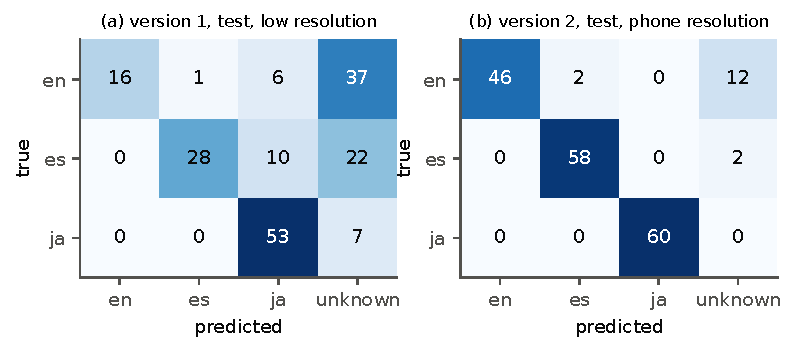
\includegraphics[width=\textwidth]{figures/language_confusion.pdf}
\caption[Language confusion matrices]{Confusion matrices of the printed-language classifier on the test split (rows: true language; columns: predicted language or ``unknown'').}
\label{fig:language-confusion}
\end{figure}

\section{Condition estimate}
\label{sec:res-condition}

Table~\ref{tab:condition} summarises the validation on synthetically damaged cards and Figure~\ref{fig:condition-example} shows an example. Centering was measured with a median error of \res{cond-centering-lr-med} (left/right) and \res{cond-centering-tb-med} (top/bottom) percentage points. Corner cuts, corner whitening and edge whitening correlated clearly with their sub-scores ($\rho$ = \res{cond-rho-corner-cut}, \res{cond-rho-corner-white}, \res{cond-rho-edge-white}), edge fraying less so ($\rho$ = \res{cond-rho-edge-fray}). Surface defects were found with a recall of \res{cond-surf-recall} and a precision of \res{cond-surf-precision}.

\begin{table}[htbp]\centering\small
\caption[Condition estimate validation]{Validation of the visual condition estimate on 80 test cards with synthetic damage of known strength (front side only). $\rho$ = Spearman rank correlation between true damage strength and the estimate.}\label{tab:condition}
\begin{tabular}{@{}lr@{}}
\toprule
Measure & Result\\
\midrule
Cards rectified / reference aligned & 80 / 76\\
Centering error L/R, median / 90th pct.\ (percentage points) & 0.58 / 2.33\\
Centering error T/B, median / 90th pct.\ (percentage points) & 0.70 / 2.33\\
$\rho$ corner cut vs.\ fill sub-score (expect $<0$) & -0.74\\
$\rho$ corner whitening vs.\ whitening sub-score & +0.62\\
$\rho$ edge whitening vs.\ whitening sub-score & +0.78\\
$\rho$ edge fray vs.\ fray sub-score & +0.41\\
Surface defects: recall / precision & 68/111 = 0.61 / 72/105 = 0.69\\
Surface defects with correct type & 59/111\\
$\rho$ part score vs.\ true damage: corners / edges / surface / centering & -0.53 / -0.32 / -0.86 / -0.90\\
$\rho$ overall score vs.\ total damage & -0.46\\
\bottomrule
\end{tabular}
\end{table}


\begin{figure}[htbp]\centering
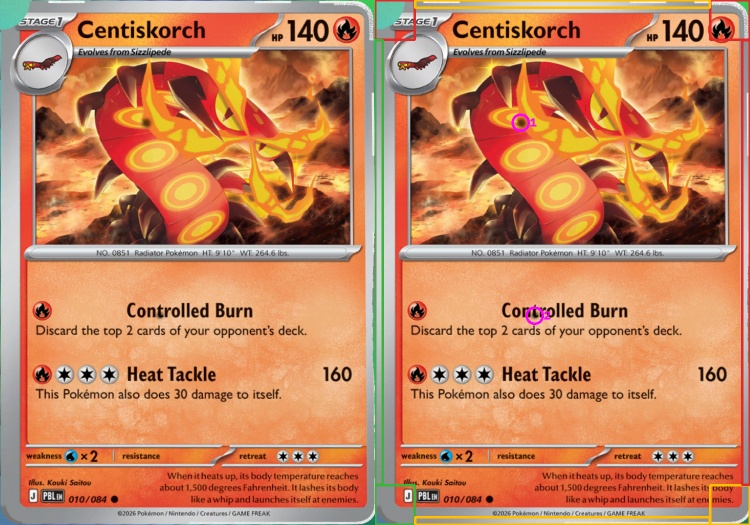
\includegraphics[width=0.85\textwidth]{figures/condition_example.jpg}
\caption[Condition estimate example]{Condition estimate on a synthetically damaged test card. Left: the rectified photo. Right: the same photo with the analysed corner and edge zones and the detected surface defects marked.}
\label{fig:condition-example}
\end{figure}

The back side could not be validated in the same way, because no official scans of card backs exist; the application's results on real photos follow in Section~\ref{sec:res-app}.

\section{The application on real photos}
\label{sec:res-app}

At the end of the project the CardDex collection contains \res{app-n-items} cards that were identified from real photos and saved by the author: \res{app-n-en} English cards and \res{app-n-ja} Japanese cards from \emph{Battle Partners} (Table~\ref{tab:app-collection}; snapshot of \res{app-snapshot-date}). Their stored prices add up to USD~\res{app-total-usd} for the English cards and EUR~\res{app-total-eur} for the Japanese cards (prices change daily; the two currencies are kept apart). Each saved card keeps the photo it was identified from (Figure~\ref{fig:app-photos}). Most of them are phone photos of cards inside protective sleeves or rigid holders, lying on a keyboard, which is a realistic and difficult setting for the detector. The Mega Chandelure is a Japanese print of a \emph{Pitch Black} card; Japanese scans of that set were not available, so it can only match its English version, and its image looks like a clean scan rather than a phone photo.

\begin{table}[htbp]\centering\footnotesize
\caption[Cards saved in the application]{Cards saved in the CardDex collection (snapshot of 2026-11-08). Price when saved: English cards = mean TCGplayer market price of the card's variants in USD; Japanese cards = Cardmarket average in EUR (both via TCGdex). Score of the saved card with the method used at save time: RANSAC inliers for SIFT, ORB and the hybrids, cosine similarity in \% for ResNet and CLIP. Condition: overall visual estimate (0--1000; mean of the two sides) and the front / back side scores as stored by the app (-- = not assessed). Lang.: printed language stored with the item.}\label{tab:app-collection}
\begin{tabular}{@{}P{1.45in}P{1.05in}cP{0.6in}rrP{1.15in}@{}}
\toprule
Card (id) & Rarity & Lang. & Method & Price & Score & Condition (overall; front / back)\\
\midrule
Mega Chandelure ex (\texttt{me5-115}) & Special Illustration Rare & en & sift & USD 32.39 & 59 & 320; 167 / 473\\
Morpeko ex (\texttt{me5-102}) & Ultra Rare & en & hybrid CLIP +rot & USD 3.52 & 285 & 258; 269 / 246\\
Goldeen (\texttt{me5-87}) & Illustration Rare & en & sift & USD 3.51 & 202 & 150; 198 / 103\\
Toucannon (\texttt{me5-94}) & Illustration Rare & en & resnet & USD 1.55 & 82.9 & 132; 162 / 103\\
Thievul (\texttt{me5-92}) & Illustration Rare & en & resnet & USD 1.31 & 76.9 & 136; 170 / 103\\
Maractus (JP) (\texttt{ja-SV9-101}) & -- & ja & sift & EUR 1.33 & 251 & 261; 220 / 302\\
Swinub (JP) (\texttt{ja-SV9-106}) & -- & ja & sift & EUR 1.60 & 290 & 189; 197 / 181\\
\bottomrule
\end{tabular}
\end{table}

\begin{figure}[htbp]\centering
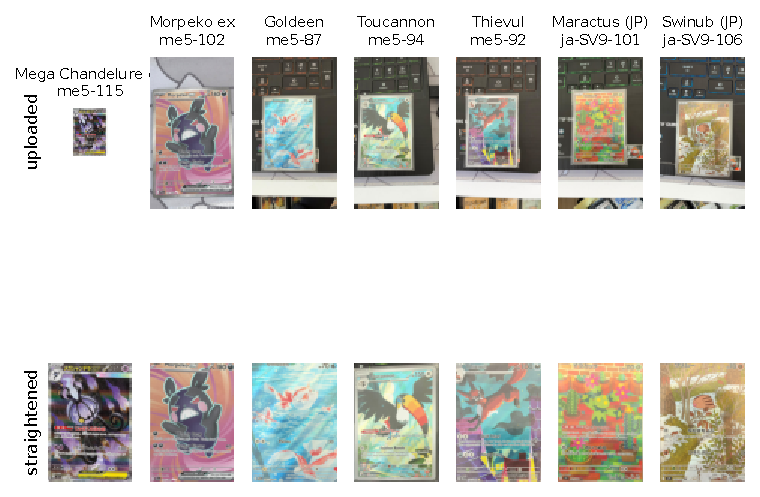
\includegraphics[width=\textwidth]{figures/app_photos.pdf}
\caption[Photos saved in the application]{The photos stored with the saved cards (top) and the card image that the application straightened from each one and passed to the retrieval method (bottom).}\label{fig:app-photos}
\end{figure}


\paragraph{Re-identification.} To turn the saved photos into a small real-photo test, every photo was identified again with each method, through the same code path as the application and against all \res{app-n-ref} reference cards of the application (\texttt{report/app\_evidence.py}). The ground truth is the card that the user saved, which the application lets the user correct before saving. Table~\ref{tab:app-reid} shows the result.
\begin{itemize}
  \item SIFT, ORB, CLIP and the CLIP hybrid ranked the exact saved card first for all \res{app-reid-n} photos, including both Japanese cards, which were matched to their Japanese scan and not to their English twin.
  \item ResNet-50 was correct for \res{app-resnet-hits} of \res{app-reid-n} photos (\res{app-resnet-hits-len} under the lenient metric): it ranked the Morpeko ex at position \res{app-resnet-me5-102-rank}, and it returned the English twin (\texttt{\res{app-resnet-ja-SV9-101-pred}}) for the Japanese Maractus.
  \item The artwork-only hybrid found the right artwork every time (\res{app-hybrid_clip@art+rot_k20-hits-len} of \res{app-reid-n} lenient) but returned the English twin for both Japanese cards (\res{app-hybrid_clip@art+rot_k20-hits} of \res{app-reid-n} strict). This is exactly what the method is designed to do: it ignores the text, and the text is the only difference between the two prints.
  \item SIFT separated the correct card clearly in every case, for example \res{app-me5-87-sift-top1} RANSAC inliers for Goldeen against \res{app-me5-87-sift-second} for the second card, and \res{app-ja-SV9-101-sift-top1} against \res{app-ja-SV9-101-sift-second} for the Japanese Maractus.
  \item Median time per photo: \res{app-sift-ms}~ms for SIFT, \res{app-orb-ms}~ms for ORB, \res{app-clip-ms}~ms for CLIP and \res{app-hybrid_clip+rot_k20-ms}~ms for the CLIP hybrid. These timings were taken while the main experiments were running on the same laptop and are only indicative.
\end{itemize}
With \res{app-reid-n} photos these numbers illustrate the behaviour on real photos but are not a statistical result.

\begin{table}[htbp]\centering\footnotesize
\caption[Re-identification of the saved photos]{Re-identification of the photos saved in the application with every method (same path as the app: rectification, then ranking of all 917 reference cards of the app, English and Japanese). Each cell is the rank of the saved card (1 = correct top-1); $\dagger$ = wrong exact card but same artwork (lenient top-1, e.g.\ the English twin of a Japanese card); bold = wrong even under the lenient metric. Ground truth = the card the user saved. Top-1 = strict / lenient. Latency: median over the photos (measured while other experiments were running, indicative only).}\label{tab:app-reid}
\begin{tabular}{@{}lcccccccrr@{}}
\toprule
Method & \rotatebox{70}{Mega Chandelure ex} & \rotatebox{70}{Morpeko ex} & \rotatebox{70}{Goldeen} & \rotatebox{70}{Toucannon} & \rotatebox{70}{Thievul} & \rotatebox{70}{Maractus (JP)} & \rotatebox{70}{Swinub (JP)} & Top-1 & ms\\
\midrule
Pixel thumbnail & 1 & 1 & \textbf{2} & 1 & \textbf{22} & \textbf{32} & \textbf{7} & 3/3 & 142\\
SIFT + RANSAC & 1 & 1 & 1 & 1 & 1 & 1 & 1 & 7/7 & 22,329\\
ORB + RANSAC & 1 & 1 & 1 & 1 & 1 & 1 & 1 & 7/7 & 7,064\\
ResNet-50 & 1 & \textbf{191} & 1 & 1 & 1 & 2$^\dagger$ & 1 & 5/6 & 275\\
CLIP ViT-B/32 & 1 & 1 & 1 & 1 & 1 & 1 & 1 & 7/7 & 270\\
Hybrid CLIP$\to$SIFT +rot & 1 & 1 & 1 & 1 & 1 & 1 & 1 & 7/7 & 1,015\\
Hybrid CLIP$\to$SIFT @art +rot & 1 & 1 & 1 & 1 & 1 & 2$^\dagger$ & 2$^\dagger$ & 5/7 & 735\\
\bottomrule
\end{tabular}
\end{table}


\paragraph{Detection on real photos.} The detector returned an outline for every saved photo, but on sleeved cards the outline is not always the card edge (Figure~\ref{fig:app-photos}): for several cards the straightened image is cropped slightly inside the card border, and for the Toucannon it includes part of the sleeve. A likely reason is that the detector keeps the strongest card-shaped rectangle, and a sleeve or rigid holder adds further rectangles just inside and outside the card edge. Identification was not affected, because the artwork and most of the card remained inside the warped image.

\paragraph{Condition estimates on real photos.} The stored condition estimates were low for every card (overall between \res{app-cond-min} and \res{app-cond-max} out of 1000), and several fronts were reported with many surface ``defects'' (for example \res{app-me5-115-front-ndefects} for the Mega Chandelure, compared with the English scan, and \res{app-ja-SV9-101-front-ndefects} for the Japanese Maractus, compared with its own Japanese scan). The Goldeen, Toucannon and Thievul have identical back scores (\res{app-me5-87-back-overall}), which suggests that the same back photo was used for the three cards. The true condition of these cards was not recorded, so the estimates cannot be scored; they are discussed in Section~\ref{sec:disc-app}.

\section{Real photos (systematic evaluation)}
\label{sec:res-real}

The planned systematic real-photo set (70--100 labelled phone photos per set under controlled variations, Section~\ref{sec:realphotos}) was not collected within the project. The real-photo evidence of this report is therefore limited to the \res{app-reid-n} photos saved in the application (Section~\ref{sec:res-app}); this is listed as a limitation in Chapter~\ref{ch:conclusions}.
  % Results (quantitative and qualitative)
\chapter{Analysis and Discussion}
\label{ch:discussion}

%-------------------------------------------------------

\section{Failure analysis}
\label{sec:failures}

Every strict top-1 failure of the single-card experiment was assigned exactly one cause by fixed rules (\texttt{cardrec/failure\_analysis.py}), checked in this order: \emph{localisation} (outline IoU $<0.5$), \emph{rectification} ($0.5 \leq$ IoU $<0.8$), \emph{upside down} (only for rotation-sensitive methods, when the true rotation lies outside the window that the warp returns upright), \emph{same artwork} (the prediction is a reprint), \emph{lookalike} (the prediction has the same name), \emph{heavy distortion} (severity 4--5 and none of the above) and \emph{other}. Because the first matching rule wins, the counts show the earliest stage at which a query went wrong, not every problem it had. Table~\ref{tab:failures} and Figure~\ref{fig:failure-causes} show the result; Figure~\ref{fig:failure-examples} shows one example per cause.

\begin{table}[htbp]\centering\small
\caption[Failure causes]{Cause of every strict top-1 failure on the synthetic single-card queries (all finished severities pooled; recomputed from the current logs). Each failure gets the first cause that applies, in the column order.}\label{tab:failures}
\begin{tabular}{@{}lrrrrrrrr@{}}
\toprule
Method & \rotatebox{70}{localization} & \rotatebox{70}{rectification} & \rotatebox{70}{upside down} & \rotatebox{70}{same artwork} & \rotatebox{70}{lookalike} & \rotatebox{70}{heavy distortion} & \rotatebox{70}{other} & \rotatebox{70}{total}\\
\midrule
Pixel thumbnail {\scriptsize(S1--5)} & 164 & 10 & 43 & 16 & 0 & 53 & 21 & 307\\
ORB + RANSAC {\scriptsize(S1--5)} & 161 & 7 & 0 & 14 & 0 & 68 & 0 & 250\\
SIFT + RANSAC {\scriptsize(S1--5)} & 156 & 6 & 0 & 18 & 1 & 60 & 9 & 250\\
ResNet-50 {\scriptsize(S1--5)} & 162 & 8 & 40 & 10 & 2 & 164 & 160 & 546\\
CLIP ViT-B/32 {\scriptsize(S1--5)} & 163 & 7 & 40 & 21 & 7 & 136 & 18 & 392\\
Hybrid ResNet$\to$SIFT {\scriptsize(S1--5)} & 161 & 8 & 31 & 15 & 2 & 117 & 44 & 378\\
Hybrid CLIP$\to$SIFT {\scriptsize(S1--5)} & 163 & 6 & 38 & 12 & 1 & 84 & 7 & 311\\
ResNet-50 +rot {\scriptsize(S1--5)} & 162 & 8 & 0 & 9 & 2 & 201 & 175 & 557\\
CLIP +rot {\scriptsize(S1--5)} & 163 & 7 & 0 & 21 & 5 & 171 & 28 & 395\\
Hybrid ResNet$\to$SIFT +rot {\scriptsize(S1--5)} & 161 & 8 & 0 & 12 & 3 & 148 & 53 & 385\\
Hybrid CLIP$\to$SIFT +rot {\scriptsize(S1--5)} & 163 & 6 & 0 & 12 & 1 & 111 & 9 & 302\\
\bottomrule
\end{tabular}
\end{table}


\begin{figure}[htbp]\centering
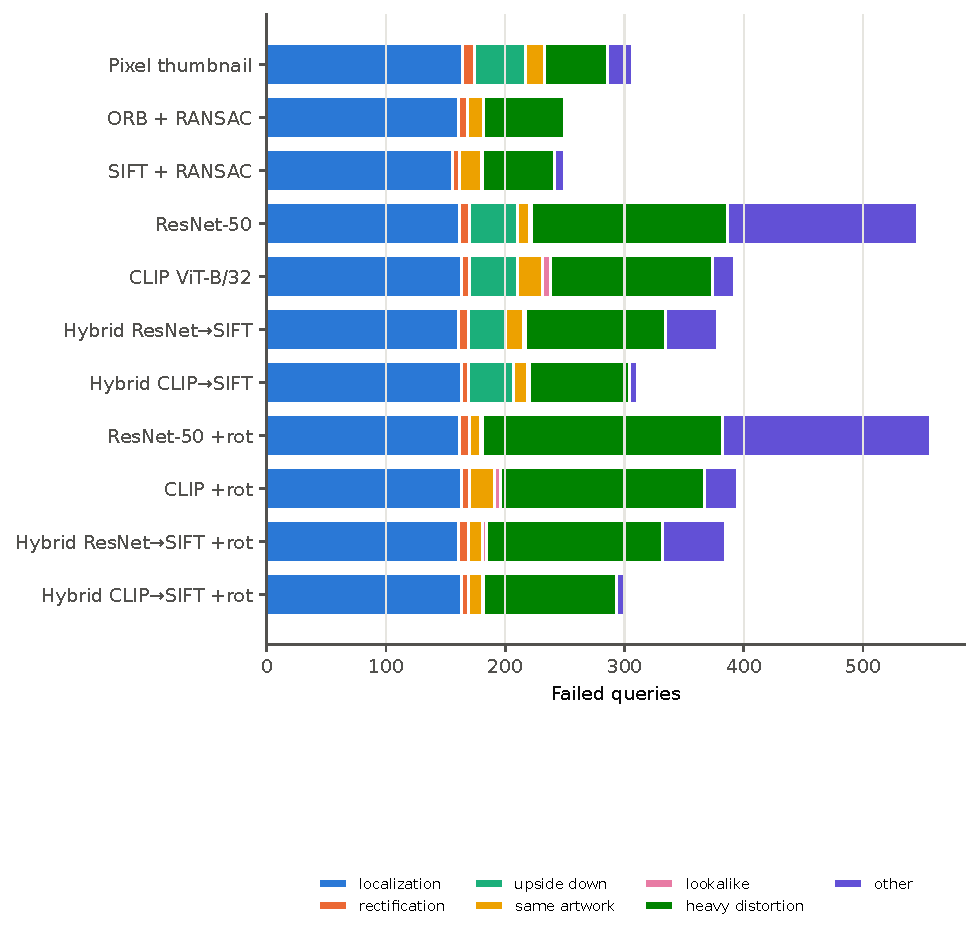
\includegraphics[width=\textwidth]{figures/failure_causes.pdf}
\caption[Failure causes per method]{Failure causes of the strict top-1 errors per method (all severities pooled, \res{main-n-queries} queries per severity).}
\label{fig:failure-causes}
\end{figure}

\begin{figure}[htbp]\centering
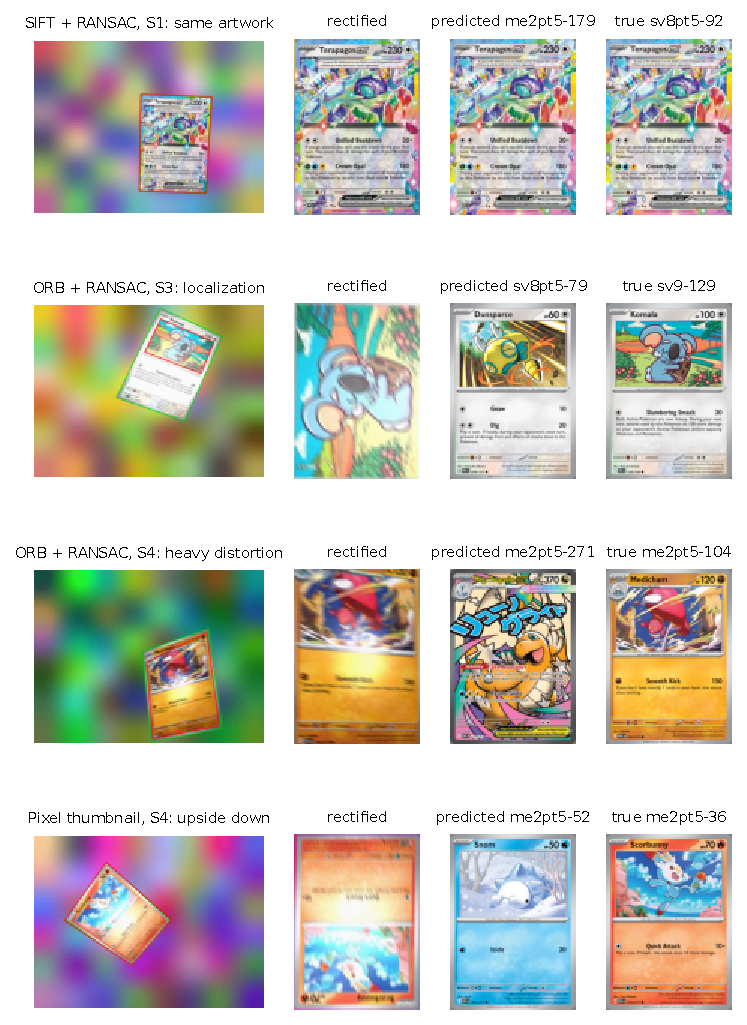
\includegraphics[width=\textwidth,height=0.8\textheight,keepaspectratio]{figures/failure_examples.pdf}
\caption[Failure examples]{Failure examples, one per row: same artwork (SIFT + RANSAC, severity 1); localization (ORB + RANSAC, severity 3); heavy distortion (ORB + RANSAC, severity 4); upside down (Pixel thumbnail, severity 4). Columns: query (green = true outline, red = detected outline), rectified card, predicted reference, true reference.}\label{fig:failure-examples}
\end{figure}


\paragraph{Localisation is the main bottleneck under strong distortion.} Every method shares the same detector and the same queries, so every method had about the same number of localisation failures (\res{fail-orb-localization} for ORB, \res{fail-clip-localization} for CLIP, \res{fail-hybrid_clip_k20-localization} for the CLIP hybrid). Of the \res{fail-orb-total} ORB failures, \res{fail-orb-localization} were localisation failures, and \res{fail-orb-s4} and \res{fail-orb-s5} of all ORB failures happened at severities 4 and 5. When the outline was wrong, identification almost never succeeded: at severity 5, ORB identified \res{orb-s5-top1_given_bad_rect} of the \res{orb-s5-nbadrect} queries with a wrong outline. When the outline was correct, ORB still reached \res{orb-s5-top1_given_rect} at severity 5 and \res{orb-s4-top1_given_rect} at severity 4. So there are two separate problems at high severity: the detector misses the card in most photos, and even a correctly rectified card is often too blurred and noisy for reliable keypoints (\res{fail-orb-heavydistortion} ORB failures are ``heavy distortion'' with a correct outline). Improving the detector (for example with a learned detector) would therefore help more than changing the retrieval method, but would not solve severity 5 alone.

\paragraph{Global embeddings also fail on well-rectified cards.} Apart from reprints, the keypoint methods did not fail when the outline was correct and the distortion moderate (ORB: \res{fail-orb-other} failures of the category ``other''). ResNet-50, in contrast, had \res{fail-resnet-other} failures of the category ``other'' (correct outline, severity 1--3, not a reprint and not a lookalike) and \res{fail-resnet-heavydistortion} ``heavy distortion'' failures, against \res{fail-clip-other} and \res{fail-clip-heavydistortion} for CLIP. A likely reason is that a frozen ImageNet descriptor summarises a card mostly by its overall colour and layout, and many cards of the same energy type and frame design look alike at that level. SIFT re-ranking repairs most of these errors: the CLIP hybrid had only \res{fail-hybrid_clip_k20-other} ``other'' failures and the ResNet hybrid \res{fail-hybrid_resnet_k20-other}.

\paragraph{Reprints and lookalikes are rare.} At severities 1 and 2, all strict errors of ORB and SIFT were reprint confusions (Section~\ref{sec:res-main}). This is expected: a reprint has the same artwork, and the only visible differences are the set symbol, the set code and the collector number in the bottom strip, which are only a few pixels tall at $500\times700$. The lenient metric shows that the method found the right \emph{artwork} in every one of these cases. A dedicated second stage that reads the collector number (OCR at higher resolution, as already done for the language) could separate them. Lookalike errors (same name, different artwork) did not occur at all for ORB and SIFT and were rare for the embeddings (\res{fail-clip-lookalike} for CLIP, \res{fail-resnet-lookalike} for ResNet-50, \res{fail-hybrid_clip_k20-lookalike} for the CLIP hybrid), so the different versions of the same Pok\'emon are distinguished well.

\paragraph{Upside-down cards.} Rotation-sensitive methods failed on cards that the warp returned upside down: \res{fail-pixel-upsidedown} times for the pixel baseline, \res{fail-resnet-upsidedown} for ResNet-50 and \res{fail-clip-upsidedown} for CLIP, all at the severities with large rotations, while ORB and SIFT had none because they are rotation invariant. The +rot variant removed these failures completely, but, as shown in Section~\ref{sec:res-main}, did not raise the overall accuracy, because other failures took their place.

\section{How realistic are the synthetic results?}
\label{sec:disc-synthetic}

The pixel-thumbnail baseline, which compares $32\times44$ grey thumbnails, identified \res{pixel-s1-top1} of the queries at severity 1 and \res{pixel-s3-top1} at severity 3, more than ResNet-50 (\res{resnet-s3-top1}) and CLIP (\res{clip-s3-top1}) alone at severity 3. Such a simple method can only work this well because each synthetic query is rendered from the \emph{same} scan that is in the database: once the card is correctly rectified, query and reference are almost the same image up to blur, noise and lighting. A real photo of a physical card differs from the scan also in printing, colour reproduction, surface reflections of holographic cards, sleeves and wear. The real photos saved in the application confirm this: there the pixel baseline identified only \res{app-pixel-hits} of the \res{app-reid-n} cards, while SIFT, ORB, CLIP and the CLIP hybrid identified all of them (Table~\ref{tab:app-reid}). The synthetic benchmark is therefore an optimistic estimate that favours pixel-level similarity; it is reliable for comparing robustness to distortion and for the ranking of the methods that use local features or learned embeddings, but the absolute numbers, and especially the strength of the pixel baseline, do not transfer to real photos.

Two further points limit the comparison across severities: each severity uses a different random set of \res{main-n-queries} cards, and the latencies were measured on a laptop that was running other jobs (including other experiments) at the same time, so they indicate orders of magnitude rather than exact times.

\section{Language, text and the global embeddings}

The cross-language experiment (Section~\ref{sec:res-language-id}) gives a first view of how the method families differ. SIFT + RANSAC was nearly language-independent, which suggests that the artwork keypoints dominate the RANSAC homography and the different text has little influence. CLIP lost accuracy on Spanish and especially Japanese cards, consistent with its embedding being influenced by the text regions; restricting it to the artwork window helped on Japanese cards but the difference is not statistically clear with \res{lang-ja-n} queries. The hybrid recovered most of the gap: the shortlist of CLIP only needs to \emph{contain} the correct card, and SIFT then picks it. Two caveats apply: the Japanese ground truth was matched by artwork similarity, so Japanese cards whose artwork differs from the English print are under-represented; and the cards were shown at severity 2 only.

The same experiment shows the cost side of the trade-off. Exhaustive SIFT took a median of \res{lang-sift-ms}~ms per photo against \res{db-cards} cards, which is too slow for interactive use and grows linearly with the database, whereas the CLIP hybrid needed about \res{lang-hybrid_clip+rot_k20-ms}~ms. The k-sweep on the main benchmark confirms the trade-off (Figure~\ref{fig:ksweep}): the CLIP hybrid reaches close to the accuracy of exhaustive keypoint matching at a fraction of its time, and its cost grows with $k$, not with the size of the database.

\section{What the application shows about real photos}
\label{sec:disc-app}

The \res{app-reid-n} photos saved in the application are too few for statistical conclusions, but they are real photos of real cards, in sleeves, and they point in clear directions.

\paragraph{Identification transfers to real photos.} SIFT, ORB, CLIP and the CLIP hybrid identified every saved photo exactly, including the two Japanese cards. ResNet-50 was again the weakest method: it failed badly on the full-art Morpeko ex, whose whole surface is illustration. With so few photos this is an indication, not proof.

\paragraph{Separate Japanese reference cards are needed for exact identification.} Adding the Japanese \emph{Battle Partners} cards to the application's database made it possible to identify a Japanese copy as the Japanese card (with its own number and price) instead of its English twin. Methods that see the whole card, text included, did this correctly; the artwork-only hybrid, which by design ignores the text, returned the English twin. The two ways of comparing cards therefore answer two different questions: ``which artwork is this?'' (artwork only, language independent) and ``which exact printing is this?'' (whole card, which needs reference scans in every language that should be recognised).

\paragraph{Sleeves move the detected outline, not the answer.} On sleeved cards the detector often locked onto a rectangle slightly inside or outside the real card edge. Identification was robust to this, but the condition estimate is not, because it measures borders, corners and edges at the outline (see below).

\paragraph{Exhaustive SIFT is too slow for the application.} With a median of \res{app-sift-ms}~ms per photo, plain SIFT, which is still the application's default method, makes the user wait many seconds (the screenshot in Figure~\ref{fig:app-screens} shows a similar time), whereas the CLIP hybrid gave the same answers in about \res{app-hybrid_clip+rot_k20-ms}~ms. This supports making the CLIP hybrid the default method. To help the user choose, the application now shows a short description of every method next to the method selector.

\paragraph{The condition estimate does not transfer to real photos yet.} On synthetic damage the estimate was validated (Section~\ref{sec:res-condition}), but on the real photos it produced uniformly low scores and many surface ``defects''. Several causes are visible in the data. (i) Reference mismatch: the front of the Japanese Mega Chandelure was compared with the \emph{English} scan, so the different text counts as damage. (ii) Real-photo conditions: the Japanese Maractus was compared with its own Japanese scan and still produced \res{app-ja-SV9-101-front-ndefects} defects, so reflections of sleeves and holders, the keyboard texture around the card and the inexact outline (above) also generate false defects and penalise edges and corners. (iii) The back side has no clean reference, so it is measured only from its own border colours, and the same back photo appears to have been reused for three cards. The estimate should therefore be presented as experimental. Fixing it requires photos of unsleeved cards on a plain background, as the application already asks for, and a comparison with the true condition of real cards.

\paragraph{Stored language.} The two \emph{Battle Partners} cards were stored with the language ``ja'', because the application now pre-selects Japanese when the matched reference card is Japanese. The Mega Chandelure, which was saved before that change, is still stored as ``en'' although it is a Japanese print; the application does not log whether a stored language came from the OCR classifier or from the user.

\section{Printed language and condition}

The language classifier improved from \res{langclf-v1-test-acc} to \res{langclf-v2-test-acc} on the test split. Version 1 failed in two ways: \res{langclf-v1-test-unknown} photos gave no usable text at low resolution (``unknown''), and \res{langclf-v1-test-falseja} English or Spanish cards were labelled Japanese because the OCR model invented kanji on blurry Latin text. Version 2 addressed both at once (higher resolution for OCR, and only kana count as Japanese evidence), so the separate contribution of each change was not measured. In version 2 almost all remaining errors are ``unknown'' answers rather than wrong languages (\res{langclf-v2-test-unknown} versus \res{langclf-v2-test-wrong}), which is the safer kind of error because the application lets the user correct it. The language-code rule decided only \res{langclf-v2-test-coderule} of the \res{langclf-v2-test-n} test photos, because the OCR model misreads the tiny code box.

For the condition estimate, centering and corner damage are measured reliably on synthetic damage, whereas edge fraying is weak ($\rho=$ \res{cond-rho-edge-fray}): fraying of less than about half a millimetre is only a few pixels wide even at 12 pixels per millimetre. The overall score correlates only moderately with the total damage ($\rho=$ \res{cond-overall}) because the weights that combine the parts are hand-set. The estimate is useful to flag visible problems, but it is not a substitute for a professional grade.
  % Analysis and discussion, failure analysis
\chapter{Conclusions, Limitations and Future Work}
\label{ch:conclusions}

%-------------------------------------------------------

\section{Conclusions}

This project built and evaluated a complete pipeline for identifying Pok\'emon trading cards in photos: a classical detector and rectifier, a reference database of \res{db-cards} English cards with reprints grouped by artwork, seven interchangeable retrieval methods with two variants, a synthetic benchmark with exact ground truth, two extensions (printed language and a visual condition estimate), and a working application that also recognises the \res{db-ja-cards} Japanese cards of \emph{Battle Partners}. The experiments support the following conclusions.
\begin{enumerate}
  \item \textbf{Local features with geometric verification are the most accurate.} At every severity the most accurate method was exhaustive ORB or SIFT with RANSAC, and the two were statistically tied with each other (severity 3: \res{orb-s3-top1} and \res{sift-s3-top1}; severity 4: \res{orb-s4-top1} and \res{sift-s4-top1}), and at mild distortion their only errors were reprints with identical artwork, which the lenient metric shows to be correct at the artwork level. Their cost is several seconds per photo, growing with the size of the database.
  \item \textbf{The CLIP hybrid is the best practical compromise.} Re-ranking a 20-card CLIP shortlist with SIFT raised CLIP from \res{clip-s3-top1} to \res{hybrid_clip_k20-s3-top1} at severity 3, matching exhaustive SIFT (\res{sift-s3-top1}) in a few hundred milliseconds per photo instead of several seconds; with $k=50$ it reached \res{ks-clip-k50-top1}. A ResNet-50 shortlist is much weaker and needs a long list ($k=50$: \res{ks-resnet-k50-top1}).
  \item \textbf{Of the frozen global embeddings, CLIP is clearly better than ResNet-50} (\res{clip-s3-top1} versus \res{resnet-s3-top1} at severity 3), but neither should be used alone for exact identification: at severities 3 and 4 both were beaten even by a $32\times44$ pixel thumbnail on the synthetic queries (\res{pixel-s3-top1} and \res{pixel-s4-top1}).
  \item \textbf{Rectification is essential, and detection is the bottleneck.} Without rectification the global methods failed almost completely at severity 3 and even the most robust method, SIFT, fell from \res{sift-s3-top1} to \res{norect-sift-top1}; under strong distortion or with overlapping cards most errors come from not finding the card outline (outline correct for only \res{rect-s5-ok}\% of the photos at severity 5; detection recall \res{sc-o30-recall} with 30\% overlap).
  \item \textbf{Trying both orientations (+rot) does not pay off}: it removes the upside-down errors but not the total number of errors.
  \item \textbf{The results transfer to real photos, except for the pixel baseline.} On the \res{app-reid-n} real photos saved in the application, SIFT, ORB, CLIP and the CLIP hybrid identified every card, including two Japanese cards that were recognised as Japanese printings, while the pixel baseline identified only \res{app-pixel-hits}. The visual condition estimate, validated on synthetic damage, does not yet give credible scores on real photos of sleeved cards.
\end{enumerate}

\section{Limitations}

\begin{itemize}
  \item \textbf{Mostly synthetic evaluation.} The benchmark uses synthetic photos rendered from the reference scans themselves, which makes the task easier than real photos (Section~\ref{sec:disc-synthetic}). The planned systematic real-photo set was not collected; the real-photo evidence is limited to the \res{app-reid-n} photos saved in the application.
  \item \textbf{Small and recent database.} \res{db-sets} English sets with \res{db-cards} cards (plus \res{db-ja-cards} Japanese cards in the application); a full collection has tens of thousands of cards, which affects both the accuracy of the global embeddings (more neighbours) and the cost of exhaustive matching.
  \item \textbf{Frozen embeddings.} ResNet-50 and CLIP were not adapted to cards, and CLIP's centre crop hides the top and bottom of the card.
  \item \textbf{Rectification ambiguity.} The rectified card can be upside down; the +rot variant removes these errors for the embedding methods but adds others.
  \item \textbf{Classical detector.} Overlapping cards merge into one contour, strong blur or glare removes the border edge, and sleeves move the detected outline.
  \item \textbf{Indicative latencies.} Timings were measured on a laptop that was running other jobs at the same time (Appendix~\ref{app:repro}).
  \item \textbf{Condition estimate.} Validated only on synthetic damage of the front side; on real photos it gave implausibly low scores, the weights are hand-set, and the score is not an official grade.
\end{itemize}

\section{Future work}

\begin{itemize}
  \item Collect and label the systematic real-photo set (varied backgrounds, lighting, glare, sleeves, several cards per photo) to confirm the ranking of the methods on real data.
  \item Separate reprints with a second stage that reads the set code and collector number at high resolution.
  \item Replace or complement the classical detector with a learned detector or segmentation model, motivated by the localisation failures, overlapping cards and sleeves.
  \item Fine-tune the global embedding on card images (for example with synthetic augmentations) so that the shortlist of the hybrid can be shorter and faster.
  \item Make the condition estimate robust to sleeves and reflections, validate it against the true condition of real cards, and add a clean reference for the card back.
  \item Make the CLIP hybrid the default method of the application, add more Japanese and other non-English sets, and log the OCR language prediction separately from the language chosen by the user.
\end{itemize}
  % Conclusions, limitations, future work
\chapter{Contribution Statement}
\label{ch:contribution}

%-------------------------------------------------------

This is an individual project. Mariana Lozano is the only team member and carried out all parts of the project: the problem definition and experimental design, the reference database and the reprint grouping, the card detection and rectification, the implementation and integration of all retrieval methods, the synthetic data generator, the evaluation and failure analysis, the language and condition extensions, the web application, and this report.

External data, libraries and pretrained models are listed in the Acknowledgments; no external code was copied into the project beyond the use of these libraries through their public interfaces.

\todo{Mariana: confirm or correct the two paragraphs above, and add the disclosure of AI assistants required by the course policy (which tools, and for which parts: code, experiments, writing).}
  % Contribution statement

%-------------------------------------------------------
\backmatter
\bibliographystyle{ascelike}
\bibliography{references}

\begin{appendices}
%%%%%%%%%%%%%%%%%%%%%%%%%%%%%%%%%%%%%%%%%%%%%%%%%%%%%
%%% APPENDIX TITLE PAGE
%%%%%%%%%%%%%%%%%%%%%%%%%%%%%%%%%%%%%%%%%%%%%%%%%%%%%

\begin{center}
\vspace*{60pt}

{\fontsize{18pt}{0pt} \MakeUppercase{\textbf{%
    Appendix A
    }}}
\vspace*{24pt}

{\fontsize{18pt}{0pt} \MakeUppercase{\textbf{%
    Reproducibility and detailed results
    }}}

\vspace*{100pt}
\end{center}
\thispagestyle{empty}
\appendix
\addtocontents{toc}{\protect\setcounter{tocdepth}{0}}
\addtocontents{toc}{\protect\renewcommand{%
    \protect\chapterprefix}{%
    \protect\hspace*{-0.5in}APPENDIX\protect\hspace*{0.6in}}}%

%%%%%%%%%%%%%%%%%%%%%%%%%%%%%%%%%%%%%%%%%%%%%%%%%%%%%
%%% APPENDIX CONTENTS
%%%%%%%%%%%%%%%%%%%%%%%%%%%%%%%%%%%%%%%%%%%%%%%%%%%%%

\chapter{Reproducibility and detailed results}
\label{app:repro}

\section{Software and hardware}

Python 3.12 on Windows 11; OpenCV, NumPy, pandas and matplotlib with the versions pinned in \texttt{requirements.txt}; PyTorch 2.11 with CUDA, torchvision 0.26, Transformers 5.20 and EasyOCR 1.7.2 for the deep-learning methods and OCR. The deep models ran on a laptop GPU (NVIDIA RTX 3050 Laptop, 4\,GB); SIFT, ORB and the detector run on the CPU. Random seeds are fixed in \texttt{cardrec/config.py}, so the query sets and splits are reproducible.

\section{Commands}

All commands are run from the project root with the project's virtual environment.
\begin{itemize}
  \item Reference database and artwork groups: \texttt{python -m cardrec.database}, \texttt{python -m cardrec.art\_groups}
  \item Synthetic experiments: \texttt{python -m cardrec.experiments --exp <name>}, with \texttt{<name>} one of \texttt{main}, \texttt{ksweep}, \texttt{norectify}, \texttt{scenes} or \texttt{all}
  \item Failure analysis: \texttt{python -m cardrec.failure\_analysis}
  \item Language: \texttt{python -m cardrec.lang\_data build|photos|eval [--split dev]}
  \item Condition validation: \texttt{python -m cardrec.condition\_eval --n 80 --split test}
  \item Real photos: \texttt{python -m cardrec.real\_photos labels|check|eval}
  \item Application: \texttt{python -m cardrec.app.server} (opens \texttt{http://127.0.0.1:5000})
  \item Application evidence (saved collection, re-identification of its photos, screenshot crops): \texttt{python report/app\_evidence.py}
  \item Tables, figures and numbers of this report: \texttt{python report/make\_figures.py}
\end{itemize}

\section{Detailed results of the main comparison}

\begin{table}[p]\centering\scriptsize\renewcommand{\arraystretch}{0.92}
\caption[All finished single-card runs]{All finished runs of the main experiment. Top-1 with 95\% bootstrap interval (1000 resamples); MRR = mean reciprocal rank (= mAP, one relevant card per query); Rect.\ ok = fraction of queries whose detected outline has IoU $\geq$ 0.8 with the true outline; Top-1$\mid$ok = top-1 among those queries; latency = median per photo (shared PC, see text).}
\label{tab:main-detail}
\begin{tabular}{@{}llcccccr@{}}
\toprule
Method & Sev. & Top-1 [95\% CI] & Top-5 & MRR & Rect.\ ok & Top-1$\mid$ok & ms \\
\midrule
Pixel thumbnail & 1 & 0.970 {\scriptsize[0.94, 0.99]} & 0.985 & 0.978 & 0.985 & 0.975 & 68\\
Pixel thumbnail & 2 & 0.930 {\scriptsize[0.90, 0.96]} & 0.960 & 0.945 & 0.990 & 0.939 & 74\\
Pixel thumbnail & 3 & 0.900 {\scriptsize[0.85, 0.94]} & 0.955 & 0.928 & 0.980 & 0.918 & 85\\
Pixel thumbnail & 4 & 0.600 {\scriptsize[0.53, 0.66]} & 0.690 & 0.639 & 0.890 & 0.674 & 95\\
Pixel thumbnail & 5 & 0.065 {\scriptsize[0.03, 0.10]} & 0.105 & 0.089 & 0.270 & 0.222 & 112\\
ORB + RANSAC & 1 & 0.995 {\scriptsize[0.98, 1.00]} & 1.000 & 0.998 & 0.985 & 0.995 & 6,109\\
ORB + RANSAC & 2 & 0.975 {\scriptsize[0.95, 0.99]} & 1.000 & 0.988 & 0.990 & 0.975 & 6,225\\
ORB + RANSAC & 3 & 0.970 {\scriptsize[0.94, 0.99]} & 0.995 & 0.983 & 0.980 & 0.974 & 6,981\\
ORB + RANSAC & 4 & 0.725 {\scriptsize[0.67, 0.79]} & 0.800 & 0.765 & 0.890 & 0.815 & 4,628\\
ORB + RANSAC & 5 & 0.085 {\scriptsize[0.05, 0.12]} & 0.130 & 0.113 & 0.270 & 0.296 & 3,340\\
SIFT + RANSAC & 1 & 0.995 {\scriptsize[0.98, 1.00]} & 1.000 & 0.998 & 0.985 & 0.995 & 33,042\\
SIFT + RANSAC & 2 & 0.970 {\scriptsize[0.94, 0.99]} & 1.000 & 0.985 & 0.990 & 0.970 & 13,298\\
SIFT + RANSAC & 3 & 0.930 {\scriptsize[0.89, 0.96]} & 0.970 & 0.952 & 0.980 & 0.934 & 8,941\\
SIFT + RANSAC & 4 & 0.745 {\scriptsize[0.69, 0.81]} & 0.785 & 0.764 & 0.890 & 0.820 & 3,141\\
SIFT + RANSAC & 5 & 0.110 {\scriptsize[0.07, 0.16]} & 0.165 & 0.136 & 0.270 & 0.333 & 1,291\\
ResNet-50 & 1 & 0.970 {\scriptsize[0.94, 0.99]} & 0.995 & 0.983 & 0.985 & 0.975 & 105\\
ResNet-50 & 2 & 0.780 {\scriptsize[0.72, 0.83]} & 0.930 & 0.849 & 0.990 & 0.788 & 108\\
ResNet-50 & 3 & 0.375 {\scriptsize[0.31, 0.45]} & 0.585 & 0.476 & 0.980 & 0.372 & 123\\
ResNet-50 & 4 & 0.120 {\scriptsize[0.07, 0.17]} & 0.260 & 0.197 & 0.890 & 0.129 & 195\\
ResNet-50 & 5 & 0.025 {\scriptsize[0.01, 0.05]} & 0.050 & 0.048 & 0.270 & 0.056 & 223\\
CLIP ViT-B/32 & 1 & 0.970 {\scriptsize[0.94, 0.99]} & 1.000 & 0.985 & 0.985 & 0.970 & 140\\
CLIP ViT-B/32 & 2 & 0.955 {\scriptsize[0.93, 0.98]} & 0.995 & 0.975 & 0.990 & 0.960 & 141\\
CLIP ViT-B/32 & 3 & 0.845 {\scriptsize[0.79, 0.90]} & 0.930 & 0.887 & 0.980 & 0.857 & 165\\
CLIP ViT-B/32 & 4 & 0.250 {\scriptsize[0.18, 0.30]} & 0.445 & 0.349 & 0.890 & 0.275 & 154\\
CLIP ViT-B/32 & 5 & 0.020 {\scriptsize[0.01, 0.04]} & 0.025 & 0.032 & 0.270 & 0.056 & 171\\
Hybrid ResNet$\to$SIFT & 1 & 0.995 {\scriptsize[0.98, 1.00]} & 1.000 & 0.998 & 0.985 & 0.995 & 710\\
Hybrid ResNet$\to$SIFT & 2 & 0.940 {\scriptsize[0.91, 0.97]} & 0.970 & 0.956 & 0.990 & 0.949 & 463\\
Hybrid ResNet$\to$SIFT & 3 & 0.755 {\scriptsize[0.69, 0.81]} & 0.790 & 0.777 & 0.980 & 0.760 & 388\\
Hybrid ResNet$\to$SIFT & 4 & 0.370 {\scriptsize[0.30, 0.44]} & 0.425 & 0.400 & 0.890 & 0.410 & 269\\
Hybrid ResNet$\to$SIFT & 5 & 0.050 {\scriptsize[0.02, 0.09]} & 0.080 & 0.070 & 0.270 & 0.148 & 230\\
Hybrid CLIP$\to$SIFT & 1 & 0.995 {\scriptsize[0.98, 1.00]} & 1.000 & 0.998 & 0.985 & 0.995 & 656\\
Hybrid CLIP$\to$SIFT & 2 & 0.965 {\scriptsize[0.94, 0.99]} & 0.995 & 0.980 & 0.990 & 0.970 & 437\\
Hybrid CLIP$\to$SIFT & 3 & 0.935 {\scriptsize[0.90, 0.96]} & 0.970 & 0.953 & 0.980 & 0.944 & 368\\
Hybrid CLIP$\to$SIFT & 4 & 0.530 {\scriptsize[0.47, 0.60]} & 0.560 & 0.553 & 0.890 & 0.584 & 260\\
Hybrid CLIP$\to$SIFT & 5 & 0.020 {\scriptsize[0.01, 0.04]} & 0.035 & 0.035 & 0.270 & 0.074 & 257\\
ResNet-50 +rot & 1 & 0.970 {\scriptsize[0.94, 0.99]} & 0.995 & 0.983 & 0.985 & 0.975 & 124\\
ResNet-50 +rot & 2 & 0.745 {\scriptsize[0.69, 0.80]} & 0.910 & 0.820 & 0.990 & 0.753 & 131\\
ResNet-50 +rot & 3 & 0.340 {\scriptsize[0.28, 0.41]} & 0.555 & 0.443 & 0.980 & 0.337 & 155\\
ResNet-50 +rot & 4 & 0.130 {\scriptsize[0.09, 0.18]} & 0.255 & 0.200 & 0.890 & 0.140 & 168\\
ResNet-50 +rot & 5 & 0.030 {\scriptsize[0.01, 0.06]} & 0.065 & 0.056 & 0.270 & 0.074 & 189\\
CLIP +rot & 1 & 0.970 {\scriptsize[0.94, 0.99]} & 1.000 & 0.985 & 0.985 & 0.970 & 135\\
CLIP +rot & 2 & 0.950 {\scriptsize[0.92, 0.98]} & 0.995 & 0.972 & 0.990 & 0.955 & 156\\
CLIP +rot & 3 & 0.810 {\scriptsize[0.76, 0.86]} & 0.920 & 0.862 & 0.980 & 0.821 & 138\\
CLIP +rot & 4 & 0.275 {\scriptsize[0.21, 0.34]} & 0.460 & 0.369 & 0.890 & 0.303 & 180\\
CLIP +rot & 5 & 0.020 {\scriptsize[0.01, 0.04]} & 0.035 & 0.036 & 0.270 & 0.056 & 201\\
Hybrid ResNet$\to$SIFT +rot & 1 & 0.995 {\scriptsize[0.98, 1.00]} & 1.000 & 0.998 & 0.985 & 0.995 & 650\\
Hybrid ResNet$\to$SIFT +rot & 2 & 0.940 {\scriptsize[0.91, 0.97]} & 0.965 & 0.954 & 0.990 & 0.949 & 489\\
Hybrid ResNet$\to$SIFT +rot & 3 & 0.715 {\scriptsize[0.65, 0.78]} & 0.750 & 0.737 & 0.980 & 0.719 & 395\\
Hybrid ResNet$\to$SIFT +rot & 4 & 0.370 {\scriptsize[0.30, 0.43]} & 0.400 & 0.394 & 0.890 & 0.410 & 286\\
Hybrid ResNet$\to$SIFT +rot & 5 & 0.055 {\scriptsize[0.03, 0.09]} & 0.090 & 0.077 & 0.270 & 0.167 & 251\\
Hybrid CLIP$\to$SIFT +rot & 1 & 0.995 {\scriptsize[0.98, 1.00]} & 1.000 & 0.998 & 0.985 & 0.995 & 678\\
Hybrid CLIP$\to$SIFT +rot & 2 & 0.965 {\scriptsize[0.94, 0.99]} & 0.995 & 0.980 & 0.990 & 0.970 & 433\\
Hybrid CLIP$\to$SIFT +rot & 3 & 0.925 {\scriptsize[0.89, 0.96]} & 0.960 & 0.943 & 0.980 & 0.934 & 365\\
Hybrid CLIP$\to$SIFT +rot & 4 & 0.565 {\scriptsize[0.50, 0.63]} & 0.585 & 0.585 & 0.890 & 0.624 & 271\\
Hybrid CLIP$\to$SIFT +rot & 5 & 0.040 {\scriptsize[0.01, 0.07]} & 0.055 & 0.056 & 0.270 & 0.148 & 245\\
\bottomrule
\end{tabular}
\end{table}


\end{appendices}


\end{document}
%-------------------------------------------------------
